% Options for packages loaded elsewhere
\PassOptionsToPackage{unicode}{hyperref}
\PassOptionsToPackage{hyphens}{url}
%
\documentclass[
  letterpaper,
  oneside,
  open=any]{scrbook}

\usepackage{amsmath,amssymb}
\usepackage{iftex}
\ifPDFTeX
  \usepackage[T1]{fontenc}
  \usepackage[utf8]{inputenc}
  \usepackage{textcomp} % provide euro and other symbols
\else % if luatex or xetex
  \usepackage{unicode-math}
  \defaultfontfeatures{Scale=MatchLowercase}
  \defaultfontfeatures[\rmfamily]{Ligatures=TeX,Scale=1}
\fi
\usepackage{lmodern}
\ifPDFTeX\else  
    % xetex/luatex font selection
\fi
% Use upquote if available, for straight quotes in verbatim environments
\IfFileExists{upquote.sty}{\usepackage{upquote}}{}
\IfFileExists{microtype.sty}{% use microtype if available
  \usepackage[]{microtype}
  \UseMicrotypeSet[protrusion]{basicmath} % disable protrusion for tt fonts
}{}
\makeatletter
\@ifundefined{KOMAClassName}{% if non-KOMA class
  \IfFileExists{parskip.sty}{%
    \usepackage{parskip}
  }{% else
    \setlength{\parindent}{0pt}
    \setlength{\parskip}{6pt plus 2pt minus 1pt}}
}{% if KOMA class
  \KOMAoptions{parskip=half}}
\makeatother
\usepackage{xcolor}
\setlength{\emergencystretch}{3em} % prevent overfull lines
\setcounter{secnumdepth}{5}
% Make \paragraph and \subparagraph free-standing
\makeatletter
\ifx\paragraph\undefined\else
  \let\oldparagraph\paragraph
  \renewcommand{\paragraph}{
    \@ifstar
      \xxxParagraphStar
      \xxxParagraphNoStar
  }
  \newcommand{\xxxParagraphStar}[1]{\oldparagraph*{#1}\mbox{}}
  \newcommand{\xxxParagraphNoStar}[1]{\oldparagraph{#1}\mbox{}}
\fi
\ifx\subparagraph\undefined\else
  \let\oldsubparagraph\subparagraph
  \renewcommand{\subparagraph}{
    \@ifstar
      \xxxSubParagraphStar
      \xxxSubParagraphNoStar
  }
  \newcommand{\xxxSubParagraphStar}[1]{\oldsubparagraph*{#1}\mbox{}}
  \newcommand{\xxxSubParagraphNoStar}[1]{\oldsubparagraph{#1}\mbox{}}
\fi
\makeatother
\usepackage{color}
\usepackage{fancyvrb}
\newcommand{\VerbBar}{|}
\newcommand{\VERB}{\Verb[commandchars=\\\{\}]}
\DefineVerbatimEnvironment{Highlighting}{Verbatim}{commandchars=\\\{\}}
% Add ',fontsize=\small' for more characters per line
\usepackage{framed}
\definecolor{shadecolor}{RGB}{241,243,245}
\newenvironment{Shaded}{\begin{snugshade}}{\end{snugshade}}
\newcommand{\AlertTok}[1]{\textcolor[rgb]{0.68,0.00,0.00}{#1}}
\newcommand{\AnnotationTok}[1]{\textcolor[rgb]{0.37,0.37,0.37}{#1}}
\newcommand{\AttributeTok}[1]{\textcolor[rgb]{0.40,0.45,0.13}{#1}}
\newcommand{\BaseNTok}[1]{\textcolor[rgb]{0.68,0.00,0.00}{#1}}
\newcommand{\BuiltInTok}[1]{\textcolor[rgb]{0.00,0.23,0.31}{#1}}
\newcommand{\CharTok}[1]{\textcolor[rgb]{0.13,0.47,0.30}{#1}}
\newcommand{\CommentTok}[1]{\textcolor[rgb]{0.37,0.37,0.37}{#1}}
\newcommand{\CommentVarTok}[1]{\textcolor[rgb]{0.37,0.37,0.37}{\textit{#1}}}
\newcommand{\ConstantTok}[1]{\textcolor[rgb]{0.56,0.35,0.01}{#1}}
\newcommand{\ControlFlowTok}[1]{\textcolor[rgb]{0.00,0.23,0.31}{\textbf{#1}}}
\newcommand{\DataTypeTok}[1]{\textcolor[rgb]{0.68,0.00,0.00}{#1}}
\newcommand{\DecValTok}[1]{\textcolor[rgb]{0.68,0.00,0.00}{#1}}
\newcommand{\DocumentationTok}[1]{\textcolor[rgb]{0.37,0.37,0.37}{\textit{#1}}}
\newcommand{\ErrorTok}[1]{\textcolor[rgb]{0.68,0.00,0.00}{#1}}
\newcommand{\ExtensionTok}[1]{\textcolor[rgb]{0.00,0.23,0.31}{#1}}
\newcommand{\FloatTok}[1]{\textcolor[rgb]{0.68,0.00,0.00}{#1}}
\newcommand{\FunctionTok}[1]{\textcolor[rgb]{0.28,0.35,0.67}{#1}}
\newcommand{\ImportTok}[1]{\textcolor[rgb]{0.00,0.46,0.62}{#1}}
\newcommand{\InformationTok}[1]{\textcolor[rgb]{0.37,0.37,0.37}{#1}}
\newcommand{\KeywordTok}[1]{\textcolor[rgb]{0.00,0.23,0.31}{\textbf{#1}}}
\newcommand{\NormalTok}[1]{\textcolor[rgb]{0.00,0.23,0.31}{#1}}
\newcommand{\OperatorTok}[1]{\textcolor[rgb]{0.37,0.37,0.37}{#1}}
\newcommand{\OtherTok}[1]{\textcolor[rgb]{0.00,0.23,0.31}{#1}}
\newcommand{\PreprocessorTok}[1]{\textcolor[rgb]{0.68,0.00,0.00}{#1}}
\newcommand{\RegionMarkerTok}[1]{\textcolor[rgb]{0.00,0.23,0.31}{#1}}
\newcommand{\SpecialCharTok}[1]{\textcolor[rgb]{0.37,0.37,0.37}{#1}}
\newcommand{\SpecialStringTok}[1]{\textcolor[rgb]{0.13,0.47,0.30}{#1}}
\newcommand{\StringTok}[1]{\textcolor[rgb]{0.13,0.47,0.30}{#1}}
\newcommand{\VariableTok}[1]{\textcolor[rgb]{0.07,0.07,0.07}{#1}}
\newcommand{\VerbatimStringTok}[1]{\textcolor[rgb]{0.13,0.47,0.30}{#1}}
\newcommand{\WarningTok}[1]{\textcolor[rgb]{0.37,0.37,0.37}{\textit{#1}}}

\providecommand{\tightlist}{%
  \setlength{\itemsep}{0pt}\setlength{\parskip}{0pt}}\usepackage{longtable,booktabs,array}
\usepackage{calc} % for calculating minipage widths
% Correct order of tables after \paragraph or \subparagraph
\usepackage{etoolbox}
\makeatletter
\patchcmd\longtable{\par}{\if@noskipsec\mbox{}\fi\par}{}{}
\makeatother
% Allow footnotes in longtable head/foot
\IfFileExists{footnotehyper.sty}{\usepackage{footnotehyper}}{\usepackage{footnote}}
\makesavenoteenv{longtable}
\usepackage{graphicx}
\makeatletter
\def\maxwidth{\ifdim\Gin@nat@width>\linewidth\linewidth\else\Gin@nat@width\fi}
\def\maxheight{\ifdim\Gin@nat@height>\textheight\textheight\else\Gin@nat@height\fi}
\makeatother
% Scale images if necessary, so that they will not overflow the page
% margins by default, and it is still possible to overwrite the defaults
% using explicit options in \includegraphics[width, height, ...]{}
\setkeys{Gin}{width=\maxwidth,height=\maxheight,keepaspectratio}
% Set default figure placement to htbp
\makeatletter
\def\fps@figure{htbp}
\makeatother

\usepackage[default]{opensans}
\fontseries{lc}\selectfont
\makeatletter
\@ifpackageloaded{bookmark}{}{\usepackage{bookmark}}
\makeatother
\makeatletter
\@ifpackageloaded{caption}{}{\usepackage{caption}}
\AtBeginDocument{%
\ifdefined\contentsname
  \renewcommand*\contentsname{Table of contents}
\else
  \newcommand\contentsname{Table of contents}
\fi
\ifdefined\listfigurename
  \renewcommand*\listfigurename{List of Figures}
\else
  \newcommand\listfigurename{List of Figures}
\fi
\ifdefined\listtablename
  \renewcommand*\listtablename{List of Tables}
\else
  \newcommand\listtablename{List of Tables}
\fi
\ifdefined\figurename
  \renewcommand*\figurename{Figure}
\else
  \newcommand\figurename{Figure}
\fi
\ifdefined\tablename
  \renewcommand*\tablename{Table}
\else
  \newcommand\tablename{Table}
\fi
}
\@ifpackageloaded{float}{}{\usepackage{float}}
\floatstyle{ruled}
\@ifundefined{c@chapter}{\newfloat{codelisting}{h}{lop}}{\newfloat{codelisting}{h}{lop}[chapter]}
\floatname{codelisting}{Listing}
\newcommand*\listoflistings{\listof{codelisting}{List of Listings}}
\makeatother
\makeatletter
\makeatother
\makeatletter
\@ifpackageloaded{caption}{}{\usepackage{caption}}
\@ifpackageloaded{subcaption}{}{\usepackage{subcaption}}
\makeatother

\usepackage{hyphenat}
\usepackage{ifthen}
\usepackage{calc}
\usepackage{calculator}

\usepackage{graphicx}
\usepackage{wallpaper}

\usepackage{geometry}

\usepackage{graphicx}
\usepackage{geometry}
\usepackage{afterpage}
\usepackage{tikz}
\usetikzlibrary{calc}
\usetikzlibrary{fadings}
\usepackage[pagecolor=none]{pagecolor}


% Set the titlepage font families







% Set the coverpage font families


\ifLuaTeX
  \usepackage{selnolig}  % disable illegal ligatures
\fi
\usepackage{bookmark}

\IfFileExists{xurl.sty}{\usepackage{xurl}}{} % add URL line breaks if available
\urlstyle{same} % disable monospaced font for URLs
\hypersetup{
  pdftitle={Analyses to support the Dolphinfish Management Strategy Evaluation in the U.S. Atlantic},
  pdfauthor={Mandy Karnauskas},
  hidelinks,
  pdfcreator={LaTeX via pandoc}}


\title{Analyses to support the Dolphinfish Management Strategy
Evaluation in the U.S. Atlantic}
\author{Mandy Karnauskas}
\date{}

\begin{document}
%%%%% begin titlepage extension code

  \begin{frontmatter}

\begin{titlepage}
% This is a combination of Pandoc templating and LaTeX
% Pandoc templating https://pandoc.org/MANUAL.html#templates
% See the README for help

\thispagestyle{empty}

\newgeometry{top=-100in}

% Page color

\newcommand{\coverauthorstyle}[1]{{\fontsize{20}{24.0}\selectfont
#1}}

\begin{tikzpicture}[remember picture, overlay, inner sep=0pt, outer sep=0pt]

\tikzfading[name=fadeout, inner color=transparent!0,outer color=transparent!100]
\tikzfading[name=fadein, inner color=transparent!100,outer color=transparent!0]
\node[anchor=south west, rotate=0.0, opacity=1.0] at ($(current page.south west)+(0pt, 8.75in)$) {

\includegraphics[width=\paperwidth, keepaspectratio]{images/cover-header-2.png}};

% Title
\newcommand{\titlelocationleft}{2.3in}
\newcommand{\titlelocationbottom}{7in}
\newcommand{\titlealign}{left}

\begin{scope}{%
\fontsize{30}{36.0}\selectfont
\node[anchor=north
west, align=left, rotate=0] (Title1) at ($(current page.south west)+(\titlelocationleft,\titlelocationbottom)$)  [text width = 5in]  {\textcolor{black}{\bfseries{\nohyphens{Analyses
to support the Dolphinfish Management Strategy Evaluation in the U.S.
Atlantic}}}};
}
\end{scope}

% Author
\newcommand{\authorlocationleft}{2.3in}
\newcommand{\authorlocationbottom}{5in}
\newcommand{\authoralign}{left}

\begin{scope}
{%
\fontsize{20}{24.0}\selectfont
\node[anchor=north
west, align=left, rotate=0] (Author1) at ($(current page.south west)+(\authorlocationleft,\authorlocationbottom)$)  [text width = 5in]  {
\coverauthorstyle{Mandy Karnauskas\\}};
}
\end{scope}

% Header
\newcommand{\headerlocationleft}{2.3in}
\newcommand{\headerlocationbottom}{9.8in}
\newcommand{\headerlocationalign}{left}

\begin{scope}
{%
\fontsize{16}{19.2}\selectfont
 \node[anchor=north west, align=left, rotate=0] (Header1) at %
($(current page.south west)+(\headerlocationleft,\headerlocationbottom)$)  [text width = 5in]  {\textcolor{white}{\nohyphens{NOAA
Technical Memorandum NMFS-XXX-\#\#}}};
}
\end{scope}

% Footer
\newcommand{\footerlocationleft}{6in}
\newcommand{\footerlocationbottom}{0.1\paperheight}
\newcommand{\footerlocationalign}{left}

\begin{scope}
{%
\fontsize{8}{9.6}\selectfont
 \node[anchor=north west, align=left, rotate=0] (Footer1) at %
($(current page.south west)+(\footerlocationleft,\footerlocationbottom)$)  [text width = 2.5in]  {{\nohyphens{U.S.
DEPARTMENT OF COMMERCE\\
\strut \\
National Oceanic and Atmospheric Administration\\
National Marine Fisheries Service\\
Northwest Fisheries Science Center}}};
}
\end{scope}

% Date
\newcommand{\datelocationleft}{6in}
\newcommand{\datelocationbottom}{2in}
\newcommand{\datelocationalign}{left}

\begin{scope}
{%
\fontsize{20}{24.0}\selectfont
 \node[anchor=north west, align=left, rotate=0] (Date1) at %
($(current page.south west)+(\datelocationleft,\datelocationbottom)$)  [text width = 2.5in]  {{\nohyphens{January
2023}}};
}
\end{scope}

\end{tikzpicture}
\clearpage
\restoregeometry
%%% TITLE PAGE START

% Set up alignment commands
%Page
\newcommand{\titlepagepagealign}{
\ifthenelse{\equal{left}{right}}{\raggedleft}{}
\ifthenelse{\equal{left}{center}}{\centering}{}
\ifthenelse{\equal{left}{left}}{\raggedright}{}
}
%% Titles
\newcommand{\titlepagetitlealign}{
\ifthenelse{\equal{left}{right}}{\raggedleft}{}
\ifthenelse{\equal{left}{center}}{\centering}{}
\ifthenelse{\equal{left}{left}}{\raggedright}{}
\ifthenelse{\equal{left}{spread}}{\makebox[\linewidth][s]}{}
}


\newcommand{\titleandsubtitle}{
% Title and subtitle
{\fontsize{30}{36.0}\selectfont
\textcolor{black}{\bfseries{\nohyphens{Analyses to support the
Dolphinfish Management Strategy Evaluation in the U.S. Atlantic}}}\par
}%
}
\newcommand{\titlepagetitleblock}{
\titleandsubtitle
}

\newcommand{\authorstyle}[1]{{\fontsize{20}{24.0}\selectfont
#1}}

\newcommand{\affiliationstyle}[1]{{#1}}

\newcommand{\titlepageauthorblock}{
{\authorstyle{\nohyphens{Mandy Karnauskas}{\textsuperscript{1}}}}}

\newcommand{\titlepageaffiliationblock}{
\hangindent=1em
\hangafter=1
{\affiliationstyle{
{1}.~NOAA Fisheres,~Southeast Fisheries Science Center


\vspace{1\baselineskip} 
}}
}
\newcommand{\headerstyled}{%
{}
}
\newcommand{\footerstyled}{%
{}
}
\newcommand{\datestyled}{%
{}
}


\newcommand{\titlepageheaderblock}{\headerstyled}

\newcommand{\titlepagefooterblock}{
\footerstyled
}

\newcommand{\titlepagedateblock}{
\datestyled
}

%set up blocks so user can specify order
\newcommand{\titleblock}{{\titlepagetitlealign

{\titlepagetitleblock}
}

\vspace{4\baselineskip}
}

\newcommand{\authorblock}{{\titlepageauthorblock}

\vspace{2\baselineskip}
}

\newcommand{\affiliationblock}{{\titlepageaffiliationblock}

\vspace{2\baselineskip}
}

\newcommand{\logoblock}{}

\newcommand{\footerblock}{}

\newcommand{\dateblock}{}

\newcommand{\headerblock}{}
\newgeometry{top=3in,bottom=1in,right=1in,left=1.75in}
% background image
\newlength{\bgimagesize}
\setlength{\bgimagesize}{0.75\paperwidth}
\LENGTHDIVIDE{\bgimagesize}{\paperwidth}{\theRatio} % from calculator pkg
\ThisULCornerWallPaper{\theRatio}{images/corner-image.png}

\thispagestyle{empty} % no page numbers on titlepages


\newcommand{\vrulecode}{\rule{\vrulewidth}{\textheight}}
\newlength{\vrulewidth}
\setlength{\vrulewidth}{0pt}
\newlength{\B}
\setlength{\B}{\ifdim\vrulewidth > 0pt 0.05\textwidth\else 0pt\fi}
\newlength{\minipagewidth}
\ifthenelse{\equal{left}{left} \OR \equal{left}{right} }
{% True case
\setlength{\minipagewidth}{\textwidth - \vrulewidth - \B - 0.1\textwidth}
}{
\setlength{\minipagewidth}{\textwidth - 2\vrulewidth - 2\B - 0.1\textwidth}
}
\ifthenelse{\equal{left}{left} \OR \equal{left}{leftright}}
{% True case
\raggedleft % needed for the minipage to work
\vrulecode
\hspace{\B}
}{%
\raggedright % else it is right only and width is not 0
}
% [position of box][box height][inner position]{width}
% [s] means stretch out vertically; assuming there is a vfill
\begin{minipage}[b][\textheight][s]{\minipagewidth}
\titlepagepagealign
\headerblock

\titleblock

\authorblock

\affiliationblock

\vfill

\logoblock

\footerblock
\par

\end{minipage}\ifthenelse{\equal{left}{right} \OR \equal{left}{leftright} }{
\hspace{\B}
\vrulecode}{}
\clearpage
\restoregeometry
%%% TITLE PAGE END
\end{titlepage}
\setcounter{page}{1}
\end{frontmatter}

%%%%% end titlepage extension code

\renewcommand*\contentsname{Table of contents}
{
\setcounter{tocdepth}{1}
\tableofcontents
}
\listoffigures
\listoftables

\mainmatter
\bookmarksetup{startatroot}

\chapter{Introduction}\label{introduction}

Here we will be displaying various data summaries and analyses related
to dolphin management in the U.S. South Atlantic.

\section{Details}\label{details}

The documentation of this data exploration was developed in R, using R
Studio and Quarto.

\bookmarksetup{startatroot}

\chapter{Defining the regions for the operating
model}\label{defining-the-regions-for-the-operating-model}

Here we define the different regions to be used in the operating model,
based on the areas that were defined in the industry working groups. The
operating model is intended to encompass the Western Central Atlantic
dolphin population and include international waters
(\href{https://www.fao.org/fishery/en/area/search}{FAO areas 21 and 31})
which are thought to be connected with the stock that is exploited by
U.S. fisheries.

We use the U.S. exclusive economic zone (EEZ) to differentiate between
national and international waters. Note that some U.S. commercial
activity occurs in high seas waters and we will account for those
catches in the summaries.

\section{Data download for the U.S.
EEZ}\label{data-download-for-the-u.s.-eez}

We download the U.S. Atlantic EEZ from
\href{https://www.marineregions.org/gazetteer.php?p=details&id=8456}{Marineregions.org}.

\begin{Shaded}
\begin{Highlighting}[]
\CommentTok{\# clear workspace and load the libraries}
\ControlFlowTok{if}\NormalTok{ (}\SpecialCharTok{!}\FunctionTok{requireNamespace}\NormalTok{(}\StringTok{"maps"}\NormalTok{, }\AttributeTok{quietly =} \ConstantTok{TRUE}\NormalTok{)) \{}
  \FunctionTok{install.packages}\NormalTok{(}\StringTok{"maps"}\NormalTok{) \}}
\FunctionTok{library}\NormalTok{(maps)}

\FunctionTok{rm}\NormalTok{(}\AttributeTok{list =} \FunctionTok{ls}\NormalTok{())}

\CommentTok{\# read in the shapefile downloaded from Marineregions.org}
\CommentTok{\#library(sf)}
\CommentTok{\#shp\_data \textless{}{-} st\_read("data/eez/eez.shp")}
\CommentTok{\#coords \textless{}{-} st\_coordinates(shp\_data)}
\CommentTok{\#co \textless{}{-} as.data.frame(coords)}
\CommentTok{\#save(co, file = "data/eez/Marineregions\_EEZ.RData")}

\FunctionTok{load}\NormalTok{(}\StringTok{"data/eez/Marineregions\_EEZ.RData"}\NormalTok{)}
\FunctionTok{head}\NormalTok{(co)}
\end{Highlighting}
\end{Shaded}

\begin{verbatim}
          X        Y L1 L2 L3
1 -67.28403 45.19125  1  1  1
2 -67.28400 45.19126  1  1  1
3 -67.28387 45.19125  1  1  1
4 -67.28383 45.19125  1  1  1
5 -67.28372 45.19125  1  1  1
6 -67.28365 45.19125  1  1  1
\end{verbatim}

\begin{Shaded}
\begin{Highlighting}[]
\FunctionTok{map}\NormalTok{(}\StringTok{"usa"}\NormalTok{, }\AttributeTok{xlim =} \FunctionTok{c}\NormalTok{(}\SpecialCharTok{{-}}\DecValTok{140}\NormalTok{, }\SpecialCharTok{{-}}\DecValTok{60}\NormalTok{), }\AttributeTok{ylim =} \FunctionTok{c}\NormalTok{(}\DecValTok{20}\NormalTok{, }\DecValTok{50}\NormalTok{))}
\FunctionTok{axis}\NormalTok{(}\DecValTok{1}\NormalTok{); }\FunctionTok{axis}\NormalTok{(}\DecValTok{2}\NormalTok{); }\FunctionTok{box}\NormalTok{()}
\FunctionTok{points}\NormalTok{(co}\SpecialCharTok{$}\NormalTok{X, co}\SpecialCharTok{$}\NormalTok{Y, }\AttributeTok{pch =} \DecValTok{19}\NormalTok{, }\AttributeTok{col =} \DecValTok{2}\NormalTok{)}

\CommentTok{\# remove points that are not in the U.S. South Atlantic}
\NormalTok{co }\OtherTok{\textless{}{-}}\NormalTok{ co[}\FunctionTok{which}\NormalTok{(co}\SpecialCharTok{$}\NormalTok{X }\SpecialCharTok{\textgreater{}}\NormalTok{ (}\SpecialCharTok{{-}}\DecValTok{82}\NormalTok{)), ]}
\NormalTok{co }\OtherTok{\textless{}{-}}\NormalTok{ co[}\SpecialCharTok{{-}}\FunctionTok{which}\NormalTok{(co}\SpecialCharTok{$}\NormalTok{X }\SpecialCharTok{\textless{}}\NormalTok{ (}\SpecialCharTok{{-}}\DecValTok{81}\NormalTok{) }\SpecialCharTok{\&}\NormalTok{ co}\SpecialCharTok{$}\NormalTok{Y }\SpecialCharTok{\textgreater{}} \DecValTok{25} \SpecialCharTok{\&}\NormalTok{ co}\SpecialCharTok{$}\NormalTok{Y }\SpecialCharTok{\textless{}} \DecValTok{28}\NormalTok{), ]}

\CommentTok{\#plot(co$X, co$Y, col = 0)}
\CommentTok{\#text(co$X, co$Y, 1:nrow(co), cex = 0.7)}
\CommentTok{\#plot(co$X, co$Y, col = 0, xlim = c({-}85, {-}80), ylim = c(22, 25))}
\CommentTok{\#text(co$X, co$Y, 1:nrow(co), cex = 0.7)}

\CommentTok{\# identify the northernmost and southernmost points along the Atlantic EEZ}
\NormalTok{co1 }\OtherTok{\textless{}{-}}\NormalTok{ co[}\DecValTok{2100}\SpecialCharTok{:}\DecValTok{3727}\NormalTok{, ]}
\FunctionTok{points}\NormalTok{(co1}\SpecialCharTok{$}\NormalTok{X, co1}\SpecialCharTok{$}\NormalTok{Y, }\AttributeTok{col =} \DecValTok{4}\NormalTok{, }\AttributeTok{pch =} \DecValTok{19}\NormalTok{)}
\end{Highlighting}
\end{Shaded}

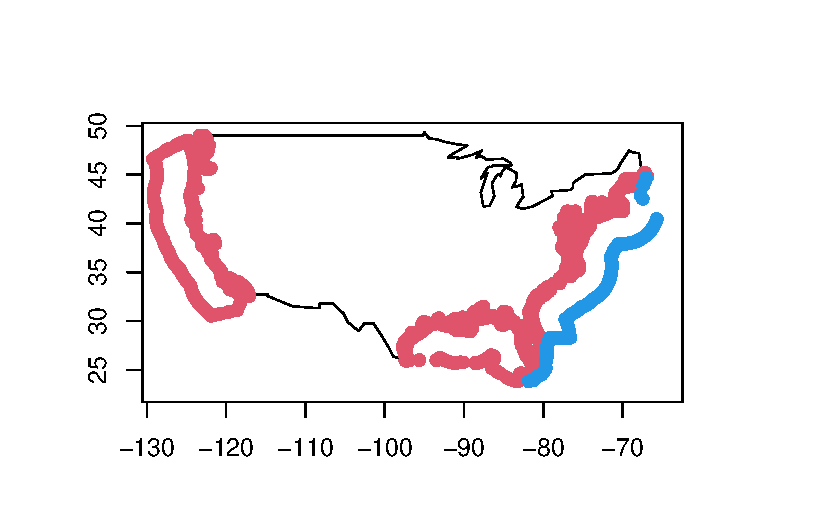
\includegraphics{makeEEZ_files/figure-pdf/unnamed-chunk-1-1.pdf}

\section{Construct the U.S. EEZ}\label{construct-the-u.s.-eez}

We simplify the shapefile along the U.S. coast in order to simplify
computations later in the process.

\begin{Shaded}
\begin{Highlighting}[]
\CommentTok{\# subset points N and S of 35N for later delineation}
\NormalTok{co2 }\OtherTok{\textless{}{-}}\NormalTok{ co[}\SpecialCharTok{{-}}\FunctionTok{c}\NormalTok{(}\DecValTok{2100}\SpecialCharTok{:}\DecValTok{3727}\NormalTok{), ]}
\NormalTok{co3 }\OtherTok{\textless{}{-}}\NormalTok{ co2[}\FunctionTok{which}\NormalTok{(co2}\SpecialCharTok{$}\NormalTok{Y }\SpecialCharTok{\textgreater{}} \DecValTok{35}\NormalTok{), ]}
\NormalTok{co4 }\OtherTok{\textless{}{-}}\NormalTok{ co2[}\FunctionTok{which}\NormalTok{(co2}\SpecialCharTok{$}\NormalTok{Y }\SpecialCharTok{\textless{}=} \DecValTok{35}\NormalTok{), ]}

\CommentTok{\# reduce number of points along the coast to make computation easier}
\NormalTok{co3 }\OtherTok{\textless{}{-}}\NormalTok{ co3[}\FunctionTok{seq}\NormalTok{(}\DecValTok{1}\NormalTok{, }\FunctionTok{nrow}\NormalTok{(co3), }\DecValTok{1100}\NormalTok{), ]}
\NormalTok{co4 }\OtherTok{\textless{}{-}}\NormalTok{ co4[}\FunctionTok{seq}\NormalTok{(}\DecValTok{1}\NormalTok{, }\FunctionTok{nrow}\NormalTok{(co4), }\DecValTok{800}\NormalTok{), ]}

\FunctionTok{map}\NormalTok{(}\StringTok{"usa"}\NormalTok{, }\AttributeTok{xlim =} \FunctionTok{c}\NormalTok{(}\SpecialCharTok{{-}}\DecValTok{100}\NormalTok{, }\SpecialCharTok{{-}}\DecValTok{60}\NormalTok{), }\AttributeTok{ylim =} \FunctionTok{c}\NormalTok{(}\DecValTok{23}\NormalTok{, }\DecValTok{50}\NormalTok{))}
\FunctionTok{mtext}\NormalTok{(}\AttributeTok{side =} \DecValTok{1}\NormalTok{, }\StringTok{"degrees W"}\NormalTok{, }\AttributeTok{line =} \DecValTok{2}\NormalTok{); }\FunctionTok{mtext}\NormalTok{(}\AttributeTok{side =} \DecValTok{2}\NormalTok{, }\StringTok{"degrees N"}\NormalTok{, }\AttributeTok{line =} \DecValTok{3}\NormalTok{)}
\FunctionTok{mtext}\NormalTok{(}\AttributeTok{side =} \DecValTok{1}\NormalTok{, }\StringTok{"degrees W"}\NormalTok{, }\AttributeTok{line =} \DecValTok{2}\NormalTok{); }\FunctionTok{mtext}\NormalTok{(}\AttributeTok{side =} \DecValTok{2}\NormalTok{, }\StringTok{"degrees N"}\NormalTok{, }\AttributeTok{line =} \DecValTok{3}\NormalTok{)}
\FunctionTok{axis}\NormalTok{(}\DecValTok{1}\NormalTok{); }\FunctionTok{axis}\NormalTok{(}\DecValTok{2}\NormalTok{); }\FunctionTok{box}\NormalTok{()}
\FunctionTok{points}\NormalTok{(co3}\SpecialCharTok{$}\NormalTok{X, co3}\SpecialCharTok{$}\NormalTok{Y, }\AttributeTok{col =} \DecValTok{2}\NormalTok{, }\AttributeTok{pch =} \DecValTok{19}\NormalTok{)}
\FunctionTok{points}\NormalTok{(co4}\SpecialCharTok{$}\NormalTok{X, co4}\SpecialCharTok{$}\NormalTok{Y, }\AttributeTok{col =} \DecValTok{4}\NormalTok{, }\AttributeTok{pch =} \DecValTok{19}\NormalTok{)}

\NormalTok{co2 }\OtherTok{\textless{}{-}} \FunctionTok{rbind}\NormalTok{(co3, co4)}
\NormalTok{co2 }\OtherTok{\textless{}{-}}\NormalTok{ co2[}\FunctionTok{order}\NormalTok{(co2}\SpecialCharTok{$}\NormalTok{Y), ]}
\NormalTok{cofin }\OtherTok{\textless{}{-}} \FunctionTok{rbind}\NormalTok{(co1, co2)}

\FunctionTok{polygon}\NormalTok{(cofin}\SpecialCharTok{$}\NormalTok{X, cofin}\SpecialCharTok{$}\NormalTok{Y, }\AttributeTok{border =} \DecValTok{5}\NormalTok{, }\AttributeTok{lwd =} \DecValTok{3}\NormalTok{)}

\CommentTok{\# make the polygon along the coast line a bit more linear}
\FunctionTok{abline}\NormalTok{(}\AttributeTok{h =} \FloatTok{37.5}\NormalTok{)}
\FunctionTok{abline}\NormalTok{(}\AttributeTok{v =} \SpecialCharTok{{-}}\DecValTok{74}\NormalTok{)}
\end{Highlighting}
\end{Shaded}

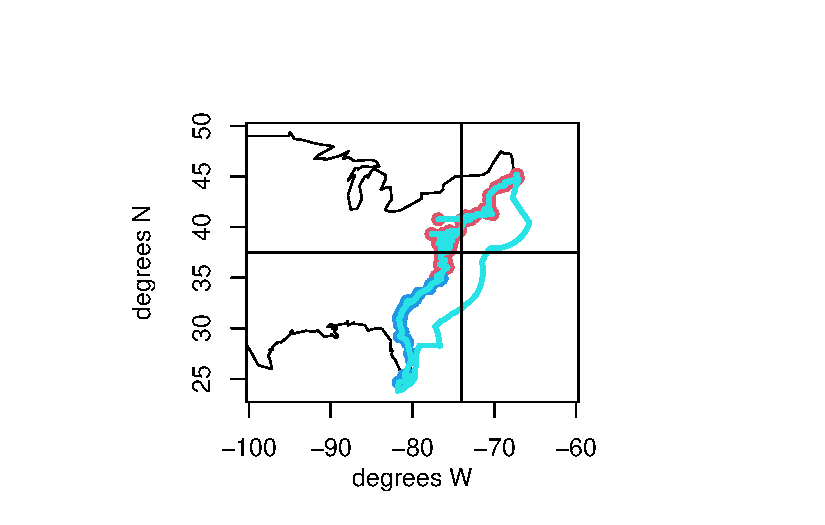
\includegraphics{makeEEZ_files/figure-pdf/unnamed-chunk-2-1.pdf}

\begin{Shaded}
\begin{Highlighting}[]
\NormalTok{cofin }\OtherTok{\textless{}{-}}\NormalTok{ cofin[}\SpecialCharTok{{-}}\FunctionTok{which}\NormalTok{(cofin}\SpecialCharTok{$}\NormalTok{X }\SpecialCharTok{\textless{}}\NormalTok{ (}\SpecialCharTok{{-}}\DecValTok{74}\NormalTok{) }\SpecialCharTok{\&}\NormalTok{ cofin}\SpecialCharTok{$}\NormalTok{Y }\SpecialCharTok{\textgreater{}} \FloatTok{37.6}\NormalTok{), ]}
\CommentTok{\#text(cofin$X, cofin$Y, 1:nrow(cofin), cex = 0.9)}
\NormalTok{lis }\OtherTok{\textless{}{-}} \FunctionTok{c}\NormalTok{(}\DecValTok{1634}\NormalTok{, }\DecValTok{1639}\NormalTok{, }\DecValTok{1688}\NormalTok{, }\DecValTok{1710}\NormalTok{, }\DecValTok{1711}\NormalTok{, }\DecValTok{1712}\NormalTok{)}
\NormalTok{cofin }\OtherTok{\textless{}{-}}\NormalTok{ cofin[}\SpecialCharTok{{-}}\NormalTok{lis, ]}

\FunctionTok{map}\NormalTok{(}\AttributeTok{database =} \StringTok{"usa"}\NormalTok{, }\AttributeTok{xlim =} \FunctionTok{c}\NormalTok{(}\SpecialCharTok{{-}}\DecValTok{70}\NormalTok{, }\SpecialCharTok{{-}}\DecValTok{65}\NormalTok{), }\AttributeTok{ylim =} \FunctionTok{c}\NormalTok{(}\DecValTok{43}\NormalTok{, }\DecValTok{47}\NormalTok{), }\AttributeTok{col =} \DecValTok{8}\NormalTok{)     }
\FunctionTok{mtext}\NormalTok{(}\AttributeTok{side =} \DecValTok{1}\NormalTok{, }\StringTok{"degrees W"}\NormalTok{, }\AttributeTok{line =} \DecValTok{2}\NormalTok{); }\FunctionTok{mtext}\NormalTok{(}\AttributeTok{side =} \DecValTok{2}\NormalTok{, }\StringTok{"degrees N"}\NormalTok{, }\AttributeTok{line =} \DecValTok{3}\NormalTok{)}
\FunctionTok{axis}\NormalTok{(}\DecValTok{1}\NormalTok{); }\FunctionTok{axis}\NormalTok{(}\DecValTok{2}\NormalTok{, }\AttributeTok{las =} \DecValTok{2}\NormalTok{); }\FunctionTok{box}\NormalTok{()}
\FunctionTok{polygon}\NormalTok{(cofin}\SpecialCharTok{$}\NormalTok{X, cofin}\SpecialCharTok{$}\NormalTok{Y, }\AttributeTok{border =} \DecValTok{2}\NormalTok{, }\AttributeTok{lwd =} \DecValTok{2}\NormalTok{)}
\FunctionTok{text}\NormalTok{(cofin}\SpecialCharTok{$}\NormalTok{X, cofin}\SpecialCharTok{$}\NormalTok{Y, }\DecValTok{1}\SpecialCharTok{:}\FunctionTok{nrow}\NormalTok{(cofin), }\AttributeTok{cex =} \FloatTok{0.9}\NormalTok{)}
\end{Highlighting}
\end{Shaded}

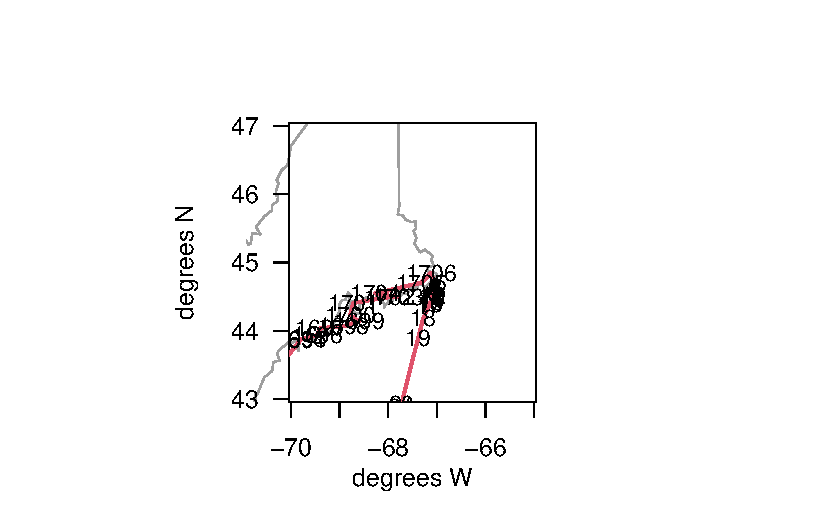
\includegraphics{makeEEZ_files/figure-pdf/unnamed-chunk-2-2.pdf}

\begin{Shaded}
\begin{Highlighting}[]
\FunctionTok{map}\NormalTok{(}\AttributeTok{database =} \StringTok{"usa"}\NormalTok{, }\AttributeTok{xlim =} \FunctionTok{c}\NormalTok{(}\SpecialCharTok{{-}}\DecValTok{72}\NormalTok{, }\SpecialCharTok{{-}}\DecValTok{71}\NormalTok{), }\AttributeTok{ylim =} \FunctionTok{c}\NormalTok{(}\FloatTok{34.8}\NormalTok{, }\FloatTok{35.1}\NormalTok{)) }
\FunctionTok{mtext}\NormalTok{(}\AttributeTok{side =} \DecValTok{1}\NormalTok{, }\StringTok{"degrees W"}\NormalTok{, }\AttributeTok{line =} \DecValTok{2}\NormalTok{); }\FunctionTok{mtext}\NormalTok{(}\AttributeTok{side =} \DecValTok{2}\NormalTok{, }\StringTok{"degrees N"}\NormalTok{, }\AttributeTok{line =} \DecValTok{3}\NormalTok{)}
\FunctionTok{axis}\NormalTok{(}\DecValTok{1}\NormalTok{); }\FunctionTok{axis}\NormalTok{(}\DecValTok{2}\NormalTok{, }\AttributeTok{las =} \DecValTok{2}\NormalTok{); }\FunctionTok{box}\NormalTok{()}
\FunctionTok{polygon}\NormalTok{(cofin}\SpecialCharTok{$}\NormalTok{X, cofin}\SpecialCharTok{$}\NormalTok{Y, }\AttributeTok{border =} \DecValTok{2}\NormalTok{)}
\FunctionTok{text}\NormalTok{(cofin}\SpecialCharTok{$}\NormalTok{X, cofin}\SpecialCharTok{$}\NormalTok{Y, }\DecValTok{1}\SpecialCharTok{:}\FunctionTok{nrow}\NormalTok{(cofin), }\AttributeTok{cex =} \FloatTok{0.6}\NormalTok{)}
\FunctionTok{abline}\NormalTok{(}\AttributeTok{h=}\DecValTok{35}\NormalTok{)}
\FunctionTok{abline}\NormalTok{(}\AttributeTok{v =} \SpecialCharTok{{-}}\DecValTok{60}\NormalTok{)}
\end{Highlighting}
\end{Shaded}

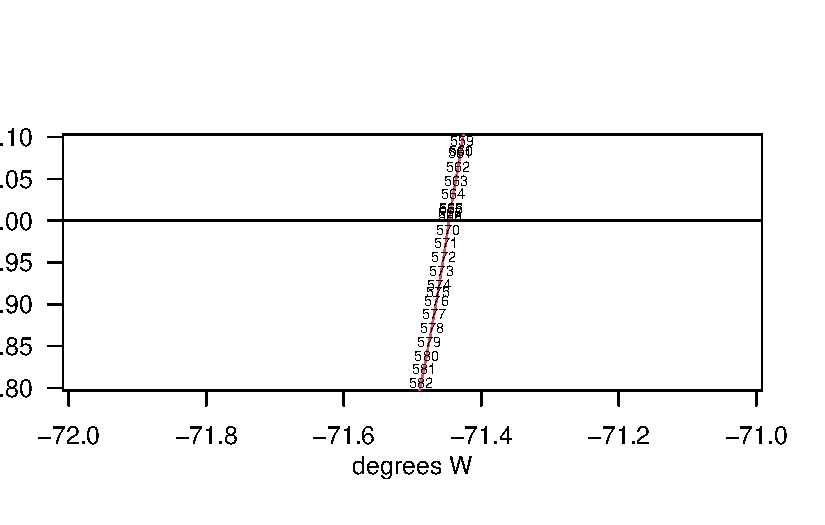
\includegraphics{makeEEZ_files/figure-pdf/unnamed-chunk-2-3.pdf}

\begin{Shaded}
\begin{Highlighting}[]
\NormalTok{cofin }\OtherTok{\textless{}{-}}\NormalTok{ cofin[, }\DecValTok{1}\SpecialCharTok{:}\DecValTok{2}\NormalTok{]}

\FunctionTok{map}\NormalTok{(}\AttributeTok{database =} \StringTok{"usa"}\NormalTok{, }\AttributeTok{xlim =} \FunctionTok{c}\NormalTok{(}\SpecialCharTok{{-}}\DecValTok{83}\NormalTok{, }\SpecialCharTok{{-}}\DecValTok{60}\NormalTok{), }\AttributeTok{ylim =} \FunctionTok{c}\NormalTok{(}\DecValTok{23}\NormalTok{, }\DecValTok{47}\NormalTok{)) }
\FunctionTok{mtext}\NormalTok{(}\AttributeTok{side =} \DecValTok{1}\NormalTok{, }\StringTok{"degrees W"}\NormalTok{, }\AttributeTok{line =} \DecValTok{2}\NormalTok{); }\FunctionTok{mtext}\NormalTok{(}\AttributeTok{side =} \DecValTok{2}\NormalTok{, }\StringTok{"degrees N"}\NormalTok{, }\AttributeTok{line =} \DecValTok{3}\NormalTok{)}
\FunctionTok{axis}\NormalTok{(}\DecValTok{1}\NormalTok{); }\FunctionTok{axis}\NormalTok{(}\DecValTok{2}\NormalTok{, }\AttributeTok{las =} \DecValTok{2}\NormalTok{); }\FunctionTok{box}\NormalTok{()}
\FunctionTok{polygon}\NormalTok{(cofin}\SpecialCharTok{$}\NormalTok{X, cofin}\SpecialCharTok{$}\NormalTok{Y, }\AttributeTok{border =} \DecValTok{2}\NormalTok{)}
\end{Highlighting}
\end{Shaded}

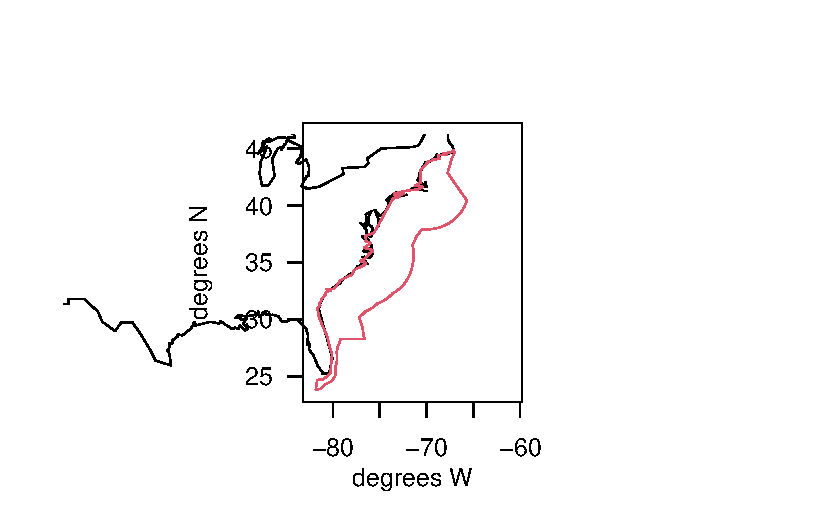
\includegraphics{makeEEZ_files/figure-pdf/unnamed-chunk-2-4.pdf}

\begin{Shaded}
\begin{Highlighting}[]
\CommentTok{\# change the southernmost tip to exactly 24N so that it alighs with Caribbean polygon}
\NormalTok{cofin }\OtherTok{\textless{}{-}}\NormalTok{ cofin[}\SpecialCharTok{{-}}\FunctionTok{which}\NormalTok{(cofin}\SpecialCharTok{$}\NormalTok{Y }\SpecialCharTok{\textless{}} \DecValTok{24}\NormalTok{), ]}
\NormalTok{cofin[}\DecValTok{1624}\NormalTok{, }\DecValTok{2}\NormalTok{] }\OtherTok{\textless{}{-}} \DecValTok{24}

\NormalTok{USeez }\OtherTok{\textless{}{-}}\NormalTok{ cofin}
\CommentTok{\#write.csv(USeez, file = "eez.csv")}
\end{Highlighting}
\end{Shaded}

Here is a final U.S. South Atlantic EEZ polygon, with a simplified
coastline to reduce computational time when subsetting data points.

\section{Define the Caribbean region}\label{define-the-caribbean-region}

Now we define the boundaries of the Caribbean region. Its northernmost
boundary aligns with the EEZ along Florida's coast up to 28.3 degrees N,
at which point the boundary cuts southeast until it intersects with the
24N boundary just east of the Bahamas, approximating the Bahamas EEX.
Its western boundary is -90 degrees W and its southern boundary is 8
degrees N (essentially the land boundary of the Caribbean Sea). Its
eastern boundary is -71.1 degrees W.

\begin{Shaded}
\begin{Highlighting}[]
\FunctionTok{which.min}\NormalTok{(cofin}\SpecialCharTok{$}\NormalTok{Y)}
\end{Highlighting}
\end{Shaded}

\begin{verbatim}
[1] 1624
\end{verbatim}

\begin{Shaded}
\begin{Highlighting}[]
\NormalTok{cofin[}\DecValTok{1624}\NormalTok{, ]}
\end{Highlighting}
\end{Shaded}

\begin{verbatim}
             X  Y
3723 -81.16148 24
\end{verbatim}

\begin{Shaded}
\begin{Highlighting}[]
\FunctionTok{map}\NormalTok{(}\AttributeTok{database =} \StringTok{"usa"}\NormalTok{, }\AttributeTok{xlim =} \FunctionTok{c}\NormalTok{(}\SpecialCharTok{{-}}\DecValTok{77}\NormalTok{, }\SpecialCharTok{{-}}\FloatTok{76.4}\NormalTok{), }\AttributeTok{ylim =} \FunctionTok{c}\NormalTok{(}\DecValTok{28}\NormalTok{, }\FloatTok{28.9}\NormalTok{))}
\FunctionTok{mtext}\NormalTok{(}\AttributeTok{side =} \DecValTok{1}\NormalTok{, }\StringTok{"degrees W"}\NormalTok{, }\AttributeTok{line =} \DecValTok{2}\NormalTok{); }\FunctionTok{mtext}\NormalTok{(}\AttributeTok{side =} \DecValTok{2}\NormalTok{, }\StringTok{"degrees N"}\NormalTok{, }\AttributeTok{line =} \DecValTok{3}\NormalTok{)}
\FunctionTok{axis}\NormalTok{(}\DecValTok{1}\NormalTok{); }\FunctionTok{axis}\NormalTok{(}\DecValTok{2}\NormalTok{, }\AttributeTok{las =} \DecValTok{2}\NormalTok{); }\FunctionTok{box}\NormalTok{()}
\FunctionTok{polygon}\NormalTok{(cofin}\SpecialCharTok{$}\NormalTok{X, cofin}\SpecialCharTok{$}\NormalTok{Y, }\AttributeTok{border =} \DecValTok{2}\NormalTok{)}
\FunctionTok{text}\NormalTok{(cofin}\SpecialCharTok{$}\NormalTok{X, cofin}\SpecialCharTok{$}\NormalTok{Y, }\DecValTok{1}\SpecialCharTok{:}\FunctionTok{nrow}\NormalTok{(cofin), }\AttributeTok{cex =} \FloatTok{0.6}\NormalTok{)}
\end{Highlighting}
\end{Shaded}

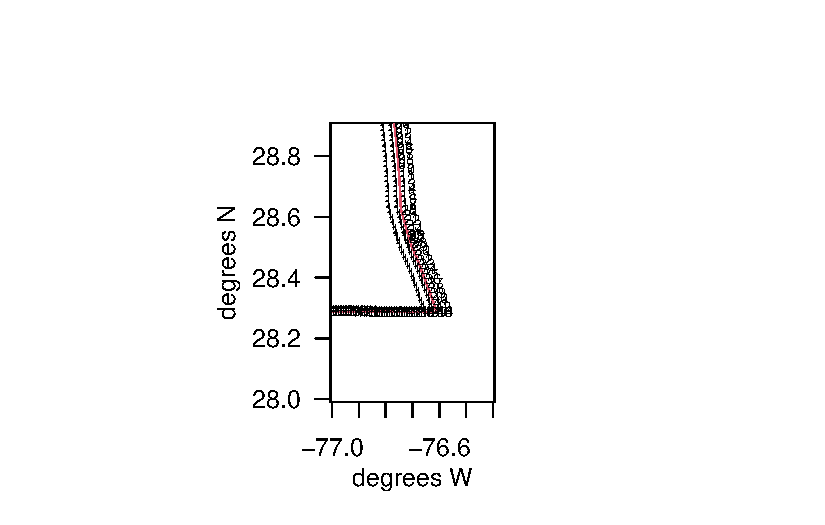
\includegraphics{makeEEZ_files/figure-pdf/unnamed-chunk-3-1.pdf}

\begin{Shaded}
\begin{Highlighting}[]
\NormalTok{car1 }\OtherTok{\textless{}{-}}\NormalTok{ cofin[}\DecValTok{1143}\SpecialCharTok{:}\DecValTok{1624}\NormalTok{, ]}
\NormalTok{car2 }\OtherTok{\textless{}{-}} \FunctionTok{data.frame}\NormalTok{(}\FunctionTok{cbind}\NormalTok{(}\FunctionTok{c}\NormalTok{(}\SpecialCharTok{{-}}\DecValTok{90}\NormalTok{, }\SpecialCharTok{{-}}\DecValTok{90}\NormalTok{, }\SpecialCharTok{{-}}\DecValTok{60}\NormalTok{, }\SpecialCharTok{{-}}\DecValTok{60}\NormalTok{, }\SpecialCharTok{{-}}\FloatTok{71.1}\NormalTok{), }\FunctionTok{c}\NormalTok{(}\DecValTok{24}\NormalTok{, }\DecValTok{8}\NormalTok{, }\DecValTok{8}\NormalTok{, }\DecValTok{24}\NormalTok{, }\DecValTok{24}\NormalTok{)))}
\FunctionTok{names}\NormalTok{(car2) }\OtherTok{\textless{}{-}} \FunctionTok{c}\NormalTok{(}\StringTok{"X"}\NormalTok{, }\StringTok{"Y"}\NormalTok{)}
\NormalTok{CAR }\OtherTok{\textless{}{-}} \FunctionTok{rbind}\NormalTok{(car1, car2)}
\FunctionTok{names}\NormalTok{(CAR) }\OtherTok{\textless{}{-}} \FunctionTok{c}\NormalTok{(}\StringTok{"X"}\NormalTok{, }\StringTok{"Y"}\NormalTok{)}

\FunctionTok{map}\NormalTok{(}\AttributeTok{database =} \StringTok{"usa"}\NormalTok{, }\AttributeTok{xlim =} \FunctionTok{c}\NormalTok{(}\SpecialCharTok{{-}}\DecValTok{95}\NormalTok{, }\SpecialCharTok{{-}}\DecValTok{60}\NormalTok{), }\AttributeTok{ylim =} \FunctionTok{c}\NormalTok{(}\DecValTok{5}\NormalTok{, }\DecValTok{36}\NormalTok{))}
\FunctionTok{mtext}\NormalTok{(}\AttributeTok{side =} \DecValTok{1}\NormalTok{, }\StringTok{"degrees W"}\NormalTok{, }\AttributeTok{line =} \DecValTok{2}\NormalTok{); }\FunctionTok{mtext}\NormalTok{(}\AttributeTok{side =} \DecValTok{2}\NormalTok{, }\StringTok{"degrees N"}\NormalTok{, }\AttributeTok{line =} \DecValTok{3}\NormalTok{)}
\FunctionTok{axis}\NormalTok{(}\DecValTok{1}\NormalTok{); }\FunctionTok{axis}\NormalTok{(}\DecValTok{2}\NormalTok{, }\AttributeTok{las =} \DecValTok{2}\NormalTok{); }\FunctionTok{box}\NormalTok{()}
\FunctionTok{polygon}\NormalTok{(CAR}\SpecialCharTok{$}\NormalTok{X, CAR}\SpecialCharTok{$}\NormalTok{Y, }\AttributeTok{col =} \DecValTok{2}\NormalTok{)}
\end{Highlighting}
\end{Shaded}

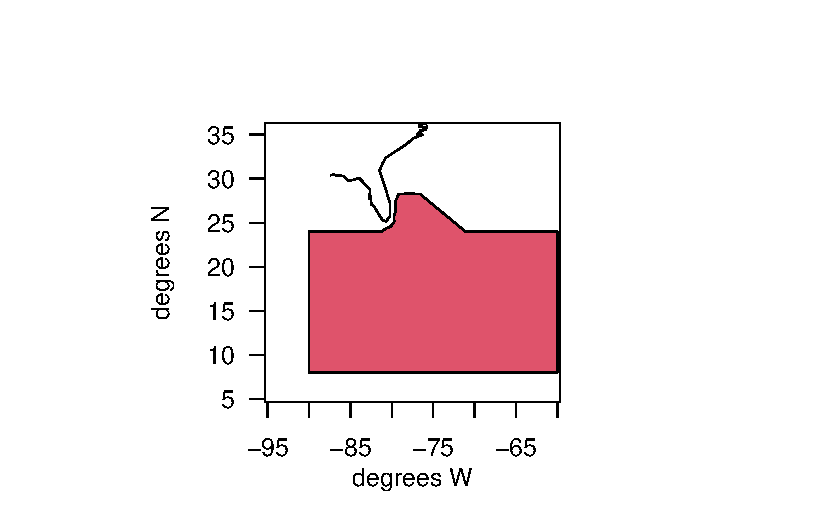
\includegraphics{makeEEZ_files/figure-pdf/unnamed-chunk-3-2.pdf}

\bookmarksetup{startatroot}

\chapter{Define the NCA region}\label{define-the-nca-region}

The North Central Atlantic (NCA) region, otherwise known as the Western
Central Atlantic, is defined according to the boundaries of FAO area
\href{https://www.fao.org/fishery/en/area/fao:31/en}{31}, but excluding
the U.S. EEZ and Caribbean territorial seas to the West.

\begin{Shaded}
\begin{Highlighting}[]
\NormalTok{nca1 }\OtherTok{\textless{}{-}}\NormalTok{ cofin[}\DecValTok{569}\SpecialCharTok{:}\DecValTok{1143}\NormalTok{, ]  }\CommentTok{\# subset points along EEZ}
\NormalTok{nca2 }\OtherTok{\textless{}{-}} \FunctionTok{data.frame}\NormalTok{(}\FunctionTok{cbind}\NormalTok{(}\FunctionTok{c}\NormalTok{(}\SpecialCharTok{{-}}\FloatTok{71.1}\NormalTok{, }\SpecialCharTok{{-}}\DecValTok{60}\NormalTok{, }\SpecialCharTok{{-}}\DecValTok{60}\NormalTok{, }\SpecialCharTok{{-}}\DecValTok{40}\NormalTok{, }\SpecialCharTok{{-}}\DecValTok{40}\NormalTok{), }\FunctionTok{c}\NormalTok{(}\DecValTok{24}\NormalTok{, }\DecValTok{24}\NormalTok{, }\DecValTok{13}\NormalTok{, }\DecValTok{13}\NormalTok{, }\DecValTok{35}\NormalTok{))) }\CommentTok{\# define boundaries according to FAO}
\FunctionTok{names}\NormalTok{(nca2) }\OtherTok{\textless{}{-}} \FunctionTok{c}\NormalTok{(}\StringTok{"X"}\NormalTok{, }\StringTok{"Y"}\NormalTok{)}
\NormalTok{NCA }\OtherTok{\textless{}{-}} \FunctionTok{rbind}\NormalTok{(nca1, nca2)}
\FunctionTok{names}\NormalTok{(NCA) }\OtherTok{\textless{}{-}} \FunctionTok{c}\NormalTok{(}\StringTok{"X"}\NormalTok{, }\StringTok{"Y"}\NormalTok{)}

\FunctionTok{map}\NormalTok{(}\AttributeTok{database =} \StringTok{"usa"}\NormalTok{, }\AttributeTok{xlim =} \FunctionTok{c}\NormalTok{(}\SpecialCharTok{{-}}\DecValTok{85}\NormalTok{, }\SpecialCharTok{{-}}\DecValTok{30}\NormalTok{), }\AttributeTok{ylim =} \FunctionTok{c}\NormalTok{(}\DecValTok{10}\NormalTok{, }\DecValTok{36}\NormalTok{)) }
\FunctionTok{mtext}\NormalTok{(}\AttributeTok{side =} \DecValTok{1}\NormalTok{, }\StringTok{"degrees W"}\NormalTok{, }\AttributeTok{line =} \DecValTok{2}\NormalTok{); }\FunctionTok{mtext}\NormalTok{(}\AttributeTok{side =} \DecValTok{2}\NormalTok{, }\StringTok{"degrees N"}\NormalTok{, }\AttributeTok{line =} \DecValTok{3}\NormalTok{)}
\FunctionTok{axis}\NormalTok{(}\DecValTok{1}\NormalTok{); }\FunctionTok{axis}\NormalTok{(}\DecValTok{2}\NormalTok{, }\AttributeTok{las =} \DecValTok{2}\NormalTok{); }\FunctionTok{box}\NormalTok{()}
\FunctionTok{polygon}\NormalTok{(NCA}\SpecialCharTok{$}\NormalTok{X, NCA}\SpecialCharTok{$}\NormalTok{Y, }\AttributeTok{col =} \DecValTok{3}\NormalTok{)}
\end{Highlighting}
\end{Shaded}

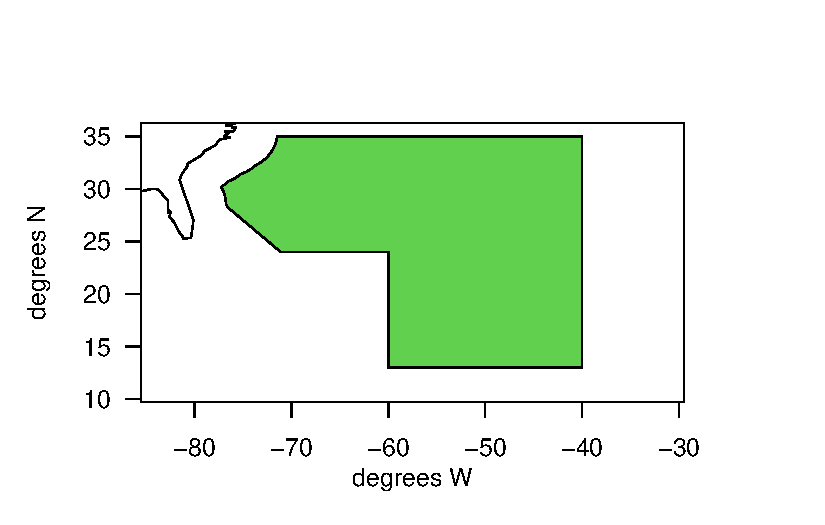
\includegraphics{makeEEZ_files/figure-pdf/unnamed-chunk-4-1.pdf}

\bookmarksetup{startatroot}

\chapter{Define the NED region}\label{define-the-ned-region}

The Northeast Distant Waters (NED) region, otherwise known as the
Northwesetern Atlantic, is defined according to the boundaries of FAO
area \href{https://www.fao.org/fishery/en/area/fao:21/en}{21}, but
excluding the U.S. EEZ territorial seas to the West. It does include
Canadian and French territorial EEZs. The northern boundary is 60
degrees north, as dolphin are not caught above this latitude.

\begin{Shaded}
\begin{Highlighting}[]
\FunctionTok{which.max}\NormalTok{(cofin}\SpecialCharTok{$}\NormalTok{Y)  }\CommentTok{\# find northernmost point of U.S. EEZ}
\end{Highlighting}
\end{Shaded}

\begin{verbatim}
[1] 1702
\end{verbatim}

\begin{Shaded}
\begin{Highlighting}[]
\NormalTok{cofin[}\DecValTok{1702}\NormalTok{, ]}
\end{Highlighting}
\end{Shaded}

\begin{verbatim}
              X        Y
77844 -67.11553 44.84764
\end{verbatim}

\begin{Shaded}
\begin{Highlighting}[]
\NormalTok{ned1 }\OtherTok{\textless{}{-}}\NormalTok{ cofin[}\DecValTok{1}\SpecialCharTok{:}\DecValTok{569}\NormalTok{, ]  }\CommentTok{\# subset points along EEZ}
\NormalTok{ned2 }\OtherTok{\textless{}{-}} \FunctionTok{data.frame}\NormalTok{(}\FunctionTok{cbind}\NormalTok{(}\FunctionTok{c}\NormalTok{(}\SpecialCharTok{{-}}\DecValTok{42}\NormalTok{, }\SpecialCharTok{{-}}\DecValTok{42}\NormalTok{, }\SpecialCharTok{{-}}\FloatTok{67.1}\NormalTok{), }\FunctionTok{c}\NormalTok{(}\DecValTok{35}\NormalTok{, }\DecValTok{55}\NormalTok{, }\DecValTok{55}\NormalTok{)))  }\CommentTok{\# define boundaries according to FAO}
\FunctionTok{names}\NormalTok{(ned2) }\OtherTok{\textless{}{-}} \FunctionTok{c}\NormalTok{(}\StringTok{"X"}\NormalTok{, }\StringTok{"Y"}\NormalTok{)}
\NormalTok{NED }\OtherTok{\textless{}{-}} \FunctionTok{rbind}\NormalTok{(ned1, ned2)}
\FunctionTok{names}\NormalTok{(NED) }\OtherTok{\textless{}{-}} \FunctionTok{c}\NormalTok{(}\StringTok{"X"}\NormalTok{, }\StringTok{"Y"}\NormalTok{)}

\FunctionTok{map}\NormalTok{(}\AttributeTok{database =} \StringTok{"usa"}\NormalTok{, }\AttributeTok{xlim =} \FunctionTok{c}\NormalTok{(}\SpecialCharTok{{-}}\DecValTok{85}\NormalTok{, }\SpecialCharTok{{-}}\DecValTok{30}\NormalTok{), }\AttributeTok{ylim =} \FunctionTok{c}\NormalTok{(}\DecValTok{30}\NormalTok{, }\DecValTok{60}\NormalTok{)) }
\FunctionTok{mtext}\NormalTok{(}\AttributeTok{side =} \DecValTok{1}\NormalTok{, }\StringTok{"degrees W"}\NormalTok{, }\AttributeTok{line =} \DecValTok{2}\NormalTok{); }\FunctionTok{mtext}\NormalTok{(}\AttributeTok{side =} \DecValTok{2}\NormalTok{, }\StringTok{"degrees N"}\NormalTok{, }\AttributeTok{line =} \DecValTok{3}\NormalTok{)}
\FunctionTok{axis}\NormalTok{(}\DecValTok{1}\NormalTok{); }\FunctionTok{axis}\NormalTok{(}\DecValTok{2}\NormalTok{, }\AttributeTok{las =} \DecValTok{2}\NormalTok{); }\FunctionTok{box}\NormalTok{()}
\FunctionTok{polygon}\NormalTok{(NED}\SpecialCharTok{$}\NormalTok{X, NED}\SpecialCharTok{$}\NormalTok{Y, }\AttributeTok{col =} \DecValTok{4}\NormalTok{)}
\end{Highlighting}
\end{Shaded}

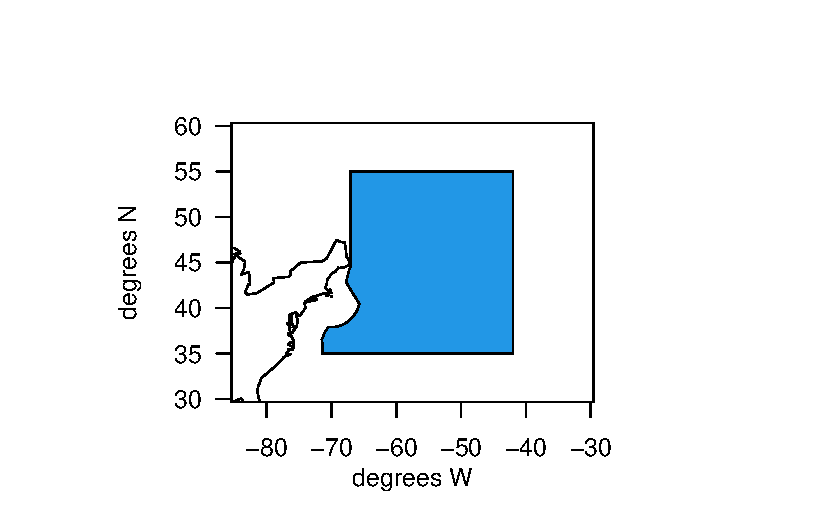
\includegraphics{makeEEZ_files/figure-pdf/unnamed-chunk-5-1.pdf}

\bookmarksetup{startatroot}

\chapter{Define the Florida Keys
region}\label{define-the-florida-keys-region}

The southernmost region of the U.S. EEZ is called the FLK region, and
includes waters within the EEZ boundary, north up to 28 degrees N. The
boundary of 28N is chosen because it aligns with commercial logbook
reporting boundaries and aligns roughly with the Brevard - Indian River
County border. This is convenient because U.S. recreational statistics
are summarized as groups of counties, with SE FL encompassing Miami-Dade
to Indian River County and NE FL encompassing Brevard to Nassau County.

\begin{Shaded}
\begin{Highlighting}[]
\FunctionTok{which.min}\NormalTok{(}\FunctionTok{abs}\NormalTok{(co1}\SpecialCharTok{$}\NormalTok{Y }\SpecialCharTok{{-}} \DecValTok{28}\NormalTok{))  }\CommentTok{\# find the southernmost point}
\end{Highlighting}
\end{Shaded}

\begin{verbatim}
[1] 1289
\end{verbatim}

\begin{Shaded}
\begin{Highlighting}[]
\FunctionTok{map}\NormalTok{(}\AttributeTok{database =} \StringTok{"usa"}\NormalTok{, }\AttributeTok{xlim =} \FunctionTok{c}\NormalTok{(}\SpecialCharTok{{-}}\DecValTok{81}\NormalTok{, }\SpecialCharTok{{-}}\DecValTok{78}\NormalTok{), }\AttributeTok{ylim =} \FunctionTok{c}\NormalTok{(}\FloatTok{27.5}\NormalTok{, }\FloatTok{28.9}\NormalTok{)) }
\FunctionTok{mtext}\NormalTok{(}\AttributeTok{side =} \DecValTok{1}\NormalTok{, }\StringTok{"degrees W"}\NormalTok{, }\AttributeTok{line =} \DecValTok{2}\NormalTok{); }\FunctionTok{mtext}\NormalTok{(}\AttributeTok{side =} \DecValTok{2}\NormalTok{, }\StringTok{"degrees N"}\NormalTok{, }\AttributeTok{line =} \DecValTok{3}\NormalTok{)}
\FunctionTok{axis}\NormalTok{(}\DecValTok{1}\NormalTok{); }\FunctionTok{axis}\NormalTok{(}\DecValTok{2}\NormalTok{, }\AttributeTok{las =} \DecValTok{2}\NormalTok{); }\FunctionTok{box}\NormalTok{()}
\FunctionTok{polygon}\NormalTok{(cofin}\SpecialCharTok{$}\NormalTok{X, cofin}\SpecialCharTok{$}\NormalTok{Y, }\AttributeTok{border =} \DecValTok{2}\NormalTok{) }
\FunctionTok{text}\NormalTok{(cofin}\SpecialCharTok{$}\NormalTok{X, cofin}\SpecialCharTok{$}\NormalTok{Y, }\DecValTok{1}\SpecialCharTok{:}\FunctionTok{nrow}\NormalTok{(cofin), }\AttributeTok{cex =} \FloatTok{0.6}\NormalTok{)   }\CommentTok{\# find points falling at 28N}
\FunctionTok{points}\NormalTok{(}\SpecialCharTok{{-}}\FloatTok{80.46}\NormalTok{, }\DecValTok{28}\NormalTok{)}
\NormalTok{cofin[}\DecValTok{1632}\NormalTok{, ] }\OtherTok{\textless{}{-}} \FunctionTok{c}\NormalTok{(}\SpecialCharTok{{-}}\FloatTok{80.46}\NormalTok{, }\DecValTok{28}\NormalTok{)}
\FunctionTok{abline}\NormalTok{(}\AttributeTok{h =} \DecValTok{28}\NormalTok{)}
\end{Highlighting}
\end{Shaded}

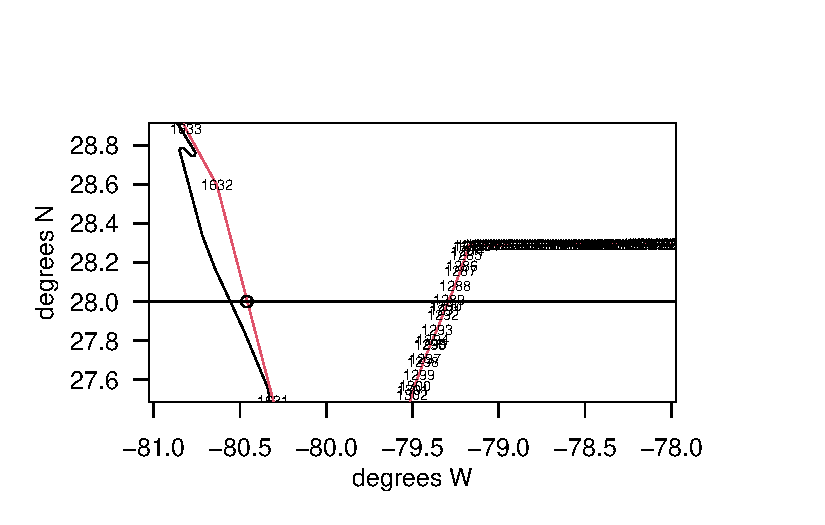
\includegraphics{makeEEZ_files/figure-pdf/unnamed-chunk-6-1.pdf}

\begin{Shaded}
\begin{Highlighting}[]
\NormalTok{FLK }\OtherTok{\textless{}{-}}\NormalTok{ cofin[}\DecValTok{1289}\SpecialCharTok{:}\DecValTok{1632}\NormalTok{, ]  }\CommentTok{\# subset points along EEZ}

\FunctionTok{map}\NormalTok{(}\AttributeTok{database =} \StringTok{"usa"}\NormalTok{, }\AttributeTok{xlim =} \FunctionTok{c}\NormalTok{(}\SpecialCharTok{{-}}\DecValTok{85}\NormalTok{, }\SpecialCharTok{{-}}\DecValTok{75}\NormalTok{), }\AttributeTok{ylim =} \FunctionTok{c}\NormalTok{(}\DecValTok{20}\NormalTok{, }\DecValTok{30}\NormalTok{)) }
\FunctionTok{mtext}\NormalTok{(}\AttributeTok{side =} \DecValTok{1}\NormalTok{, }\StringTok{"degrees W"}\NormalTok{, }\AttributeTok{line =} \DecValTok{2}\NormalTok{); }\FunctionTok{mtext}\NormalTok{(}\AttributeTok{side =} \DecValTok{2}\NormalTok{, }\StringTok{"degrees N"}\NormalTok{, }\AttributeTok{line =} \DecValTok{3}\NormalTok{)}
\FunctionTok{axis}\NormalTok{(}\DecValTok{1}\NormalTok{); }\FunctionTok{axis}\NormalTok{(}\DecValTok{2}\NormalTok{, }\AttributeTok{las =} \DecValTok{2}\NormalTok{); }\FunctionTok{box}\NormalTok{()}
\FunctionTok{polygon}\NormalTok{(FLK}\SpecialCharTok{$}\NormalTok{X, FLK}\SpecialCharTok{$}\NormalTok{Y, }\AttributeTok{col =} \DecValTok{4}\NormalTok{)}
\end{Highlighting}
\end{Shaded}

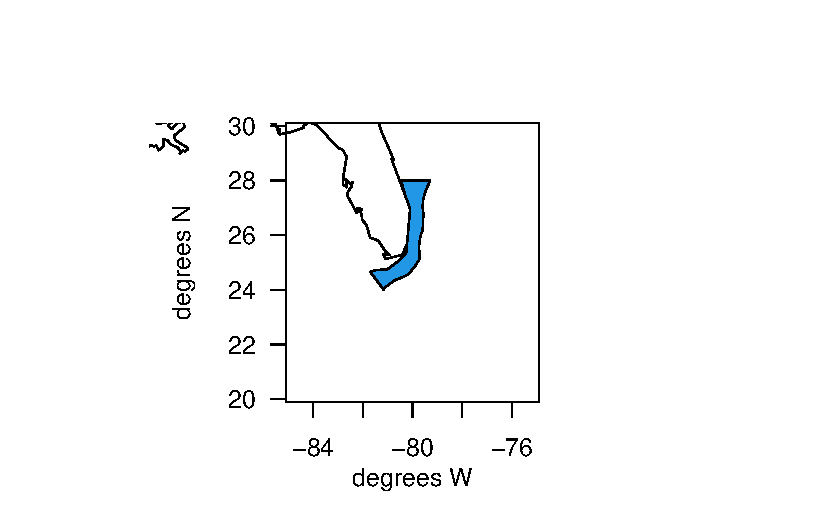
\includegraphics{makeEEZ_files/figure-pdf/unnamed-chunk-6-2.pdf}

\bookmarksetup{startatroot}

\chapter{Define the North Florida - South NC
region}\label{define-the-north-florida---south-nc-region}

The second area that was decided upon to be defined within the operating
model was northern Florida to Southern North Carolina. We form a
boundary at 35 degrees north because this is the delineation between the
NED and NCA regions. Also, 35N is just south of Cape Hatteras, which is
a boundary for NMFS recreational data collection, as well as a boundary
of commercial logbook data reporting. Therefore, all sources of data
(international, U.S. commercial, and U.S. recreational) can be easily
parsed along this boundary.

\begin{Shaded}
\begin{Highlighting}[]
\FunctionTok{map}\NormalTok{(}\AttributeTok{database =} \StringTok{"usa"}\NormalTok{, }\AttributeTok{xlim =} \FunctionTok{c}\NormalTok{(}\SpecialCharTok{{-}}\DecValTok{72}\NormalTok{, }\SpecialCharTok{{-}}\DecValTok{70}\NormalTok{), }\AttributeTok{ylim =} \FunctionTok{c}\NormalTok{(}\FloatTok{34.5}\NormalTok{, }\FloatTok{35.4}\NormalTok{))}
\FunctionTok{mtext}\NormalTok{(}\AttributeTok{side =} \DecValTok{1}\NormalTok{, }\StringTok{"degrees W"}\NormalTok{, }\AttributeTok{line =} \DecValTok{2}\NormalTok{); }\FunctionTok{mtext}\NormalTok{(}\AttributeTok{side =} \DecValTok{2}\NormalTok{, }\StringTok{"degrees N"}\NormalTok{, }\AttributeTok{line =} \DecValTok{3}\NormalTok{)}
\FunctionTok{axis}\NormalTok{(}\DecValTok{1}\NormalTok{); }\FunctionTok{axis}\NormalTok{(}\DecValTok{2}\NormalTok{, }\AttributeTok{las =} \DecValTok{2}\NormalTok{); }\FunctionTok{box}\NormalTok{()}
\FunctionTok{polygon}\NormalTok{(cofin}\SpecialCharTok{$}\NormalTok{X, cofin}\SpecialCharTok{$}\NormalTok{Y, }\AttributeTok{border =} \DecValTok{2}\NormalTok{)}
\FunctionTok{text}\NormalTok{(cofin}\SpecialCharTok{$}\NormalTok{X, cofin}\SpecialCharTok{$}\NormalTok{Y, }\DecValTok{1}\SpecialCharTok{:}\FunctionTok{nrow}\NormalTok{(cofin), }\AttributeTok{cex =} \FloatTok{0.6}\NormalTok{)  }\CommentTok{\# find points that fall at 35N}
\FunctionTok{abline}\NormalTok{(}\AttributeTok{h =} \DecValTok{35}\NormalTok{)}
\end{Highlighting}
\end{Shaded}

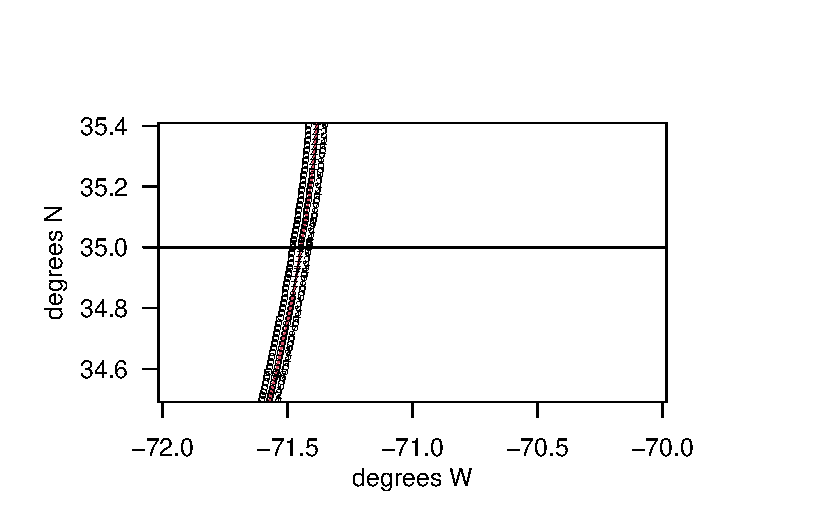
\includegraphics{makeEEZ_files/figure-pdf/unnamed-chunk-7-1.pdf}

\begin{Shaded}
\begin{Highlighting}[]
\NormalTok{cofin[}\DecValTok{1663}\NormalTok{, }\DecValTok{2}\NormalTok{] }\OtherTok{\textless{}{-}} \DecValTok{35}
\NormalTok{NCFL }\OtherTok{\textless{}{-}} \FunctionTok{rbind}\NormalTok{(cofin[}\DecValTok{1632}\SpecialCharTok{:}\DecValTok{1663}\NormalTok{, ], cofin[}\DecValTok{569}\SpecialCharTok{:}\DecValTok{1289}\NormalTok{, ])  }\CommentTok{\# subset along EEZ}

\FunctionTok{map}\NormalTok{(}\AttributeTok{database =} \StringTok{"usa"}\NormalTok{, }\AttributeTok{xlim =} \FunctionTok{c}\NormalTok{(}\SpecialCharTok{{-}}\DecValTok{85}\NormalTok{, }\SpecialCharTok{{-}}\DecValTok{70}\NormalTok{), }\AttributeTok{ylim =} \FunctionTok{c}\NormalTok{(}\DecValTok{25}\NormalTok{, }\DecValTok{40}\NormalTok{)) }
\FunctionTok{mtext}\NormalTok{(}\AttributeTok{side =} \DecValTok{1}\NormalTok{, }\StringTok{"degrees W"}\NormalTok{, }\AttributeTok{line =} \DecValTok{2}\NormalTok{); }\FunctionTok{mtext}\NormalTok{(}\AttributeTok{side =} \DecValTok{2}\NormalTok{, }\StringTok{"degrees N"}\NormalTok{, }\AttributeTok{line =} \DecValTok{3}\NormalTok{)}
\FunctionTok{axis}\NormalTok{(}\DecValTok{1}\NormalTok{); }\FunctionTok{axis}\NormalTok{(}\DecValTok{2}\NormalTok{, }\AttributeTok{las =} \DecValTok{2}\NormalTok{); }\FunctionTok{box}\NormalTok{()}
\FunctionTok{polygon}\NormalTok{(NCFL}\SpecialCharTok{$}\NormalTok{X, NCFL}\SpecialCharTok{$}\NormalTok{Y, }\AttributeTok{col =} \DecValTok{4}\NormalTok{)}
\end{Highlighting}
\end{Shaded}

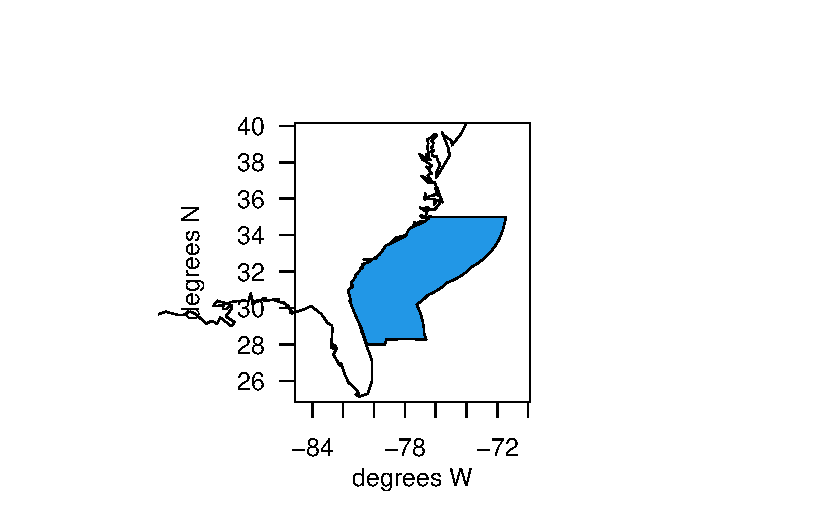
\includegraphics{makeEEZ_files/figure-pdf/unnamed-chunk-7-2.pdf}

\bookmarksetup{startatroot}

\chapter{Define the northern North Carolina
region}\label{define-the-northern-north-carolina-region}

The third U.S. area that was decided upon to be defined within the
operating model was northern North Carolina, which was intended to
encompass the northern part of the state up to the Virginia border. We
form a boundary at 37 degrees north because this is a boundary for
commercial logbook data reporting and roughly aligns with the latitude
of the state boundary between North Carolina and Virginia. Note there is
a slight misalignment between this boundary and the way that U.S.
recreational statistics are reported (by state), so the commercial and
recreational data will be subset along slightly different boundaries for
this region.

\begin{Shaded}
\begin{Highlighting}[]
\FunctionTok{map}\NormalTok{(}\AttributeTok{database =} \StringTok{"usa"}\NormalTok{, }\AttributeTok{xlim =} \FunctionTok{c}\NormalTok{(}\SpecialCharTok{{-}}\DecValTok{72}\NormalTok{, }\SpecialCharTok{{-}}\DecValTok{70}\NormalTok{), }\AttributeTok{ylim =} \FunctionTok{c}\NormalTok{(}\FloatTok{36.5}\NormalTok{, }\FloatTok{37.4}\NormalTok{))}
\FunctionTok{mtext}\NormalTok{(}\AttributeTok{side =} \DecValTok{1}\NormalTok{, }\StringTok{"degrees W"}\NormalTok{, }\AttributeTok{line =} \DecValTok{2}\NormalTok{); }\FunctionTok{mtext}\NormalTok{(}\AttributeTok{side =} \DecValTok{2}\NormalTok{, }\StringTok{"degrees N"}\NormalTok{, }\AttributeTok{line =} \DecValTok{3}\NormalTok{)}
\FunctionTok{axis}\NormalTok{(}\DecValTok{1}\NormalTok{); }\FunctionTok{axis}\NormalTok{(}\DecValTok{2}\NormalTok{, }\AttributeTok{las =} \DecValTok{2}\NormalTok{); }\FunctionTok{box}\NormalTok{()}
\FunctionTok{polygon}\NormalTok{(cofin}\SpecialCharTok{$}\NormalTok{X, cofin}\SpecialCharTok{$}\NormalTok{Y, }\AttributeTok{border =} \DecValTok{2}\NormalTok{)}
\FunctionTok{text}\NormalTok{(cofin}\SpecialCharTok{$}\NormalTok{X, cofin}\SpecialCharTok{$}\NormalTok{Y, }\DecValTok{1}\SpecialCharTok{:}\FunctionTok{nrow}\NormalTok{(cofin), }\AttributeTok{cex =} \FloatTok{0.6}\NormalTok{)}
\FunctionTok{abline}\NormalTok{(}\AttributeTok{h =} \DecValTok{37}\NormalTok{)}
\end{Highlighting}
\end{Shaded}

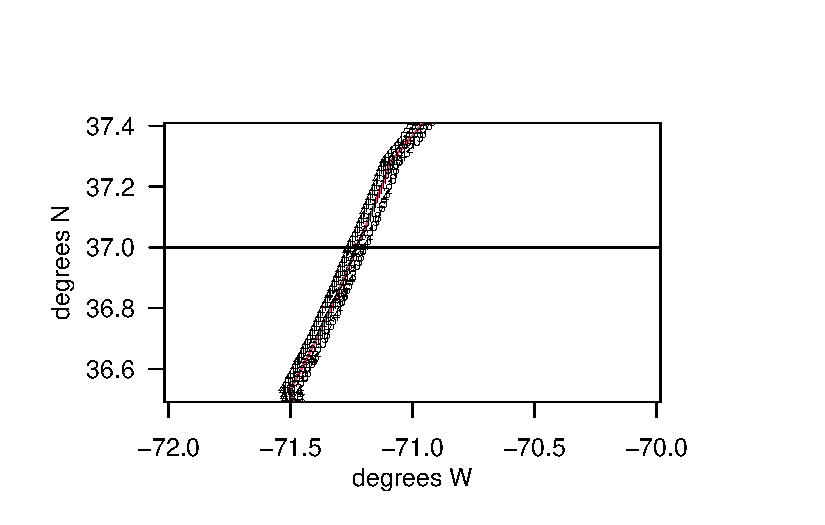
\includegraphics{makeEEZ_files/figure-pdf/unnamed-chunk-8-1.pdf}

\begin{Shaded}
\begin{Highlighting}[]
\NormalTok{cofin[}\DecValTok{425}\NormalTok{, }\DecValTok{2}\NormalTok{] }\OtherTok{\textless{}{-}} \DecValTok{37}
\NormalTok{NNC }\OtherTok{\textless{}{-}} \FunctionTok{rbind}\NormalTok{(cofin[}\DecValTok{1663}\SpecialCharTok{:}\DecValTok{1673}\NormalTok{, ], cofin[}\DecValTok{425}\SpecialCharTok{:}\DecValTok{569}\NormalTok{, ])}

\FunctionTok{map}\NormalTok{(}\AttributeTok{database =} \StringTok{"usa"}\NormalTok{, }\AttributeTok{xlim =} \FunctionTok{c}\NormalTok{(}\SpecialCharTok{{-}}\DecValTok{85}\NormalTok{, }\SpecialCharTok{{-}}\DecValTok{70}\NormalTok{), }\AttributeTok{ylim =} \FunctionTok{c}\NormalTok{(}\DecValTok{25}\NormalTok{, }\DecValTok{40}\NormalTok{))}
\FunctionTok{mtext}\NormalTok{(}\AttributeTok{side =} \DecValTok{1}\NormalTok{, }\StringTok{"degrees W"}\NormalTok{, }\AttributeTok{line =} \DecValTok{2}\NormalTok{); }\FunctionTok{mtext}\NormalTok{(}\AttributeTok{side =} \DecValTok{2}\NormalTok{, }\StringTok{"degrees N"}\NormalTok{, }\AttributeTok{line =} \DecValTok{3}\NormalTok{)}
\FunctionTok{axis}\NormalTok{(}\DecValTok{1}\NormalTok{); }\FunctionTok{axis}\NormalTok{(}\DecValTok{2}\NormalTok{, }\AttributeTok{las =} \DecValTok{2}\NormalTok{); }\FunctionTok{box}\NormalTok{()}
\FunctionTok{polygon}\NormalTok{(NNC}\SpecialCharTok{$}\NormalTok{X, NNC}\SpecialCharTok{$}\NormalTok{Y, }\AttributeTok{col =} \DecValTok{4}\NormalTok{)}
\end{Highlighting}
\end{Shaded}

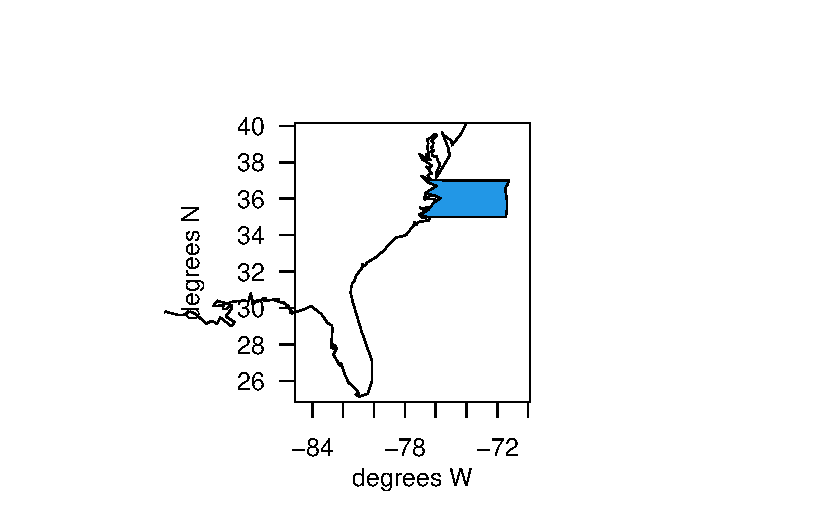
\includegraphics{makeEEZ_files/figure-pdf/unnamed-chunk-8-2.pdf}

\bookmarksetup{startatroot}

\chapter{Define the Virginia and north
region}\label{define-the-virginia-and-north-region}

The fourth region within the U.S. EEZ is the remainder of the area,
which encompasses national waters from Virginia up to Maine.

\begin{Shaded}
\begin{Highlighting}[]
\NormalTok{VBM }\OtherTok{\textless{}{-}} \FunctionTok{rbind}\NormalTok{(cofin[}\DecValTok{1673}\SpecialCharTok{:}\DecValTok{1702}\NormalTok{, ], cofin[}\DecValTok{1}\SpecialCharTok{:}\DecValTok{425}\NormalTok{, ])}

\FunctionTok{map}\NormalTok{(}\AttributeTok{database =} \StringTok{"usa"}\NormalTok{, }\AttributeTok{xlim =} \FunctionTok{c}\NormalTok{(}\SpecialCharTok{{-}}\DecValTok{80}\NormalTok{, }\SpecialCharTok{{-}}\DecValTok{60}\NormalTok{), }\AttributeTok{ylim =} \FunctionTok{c}\NormalTok{(}\DecValTok{30}\NormalTok{, }\DecValTok{50}\NormalTok{)) }
\FunctionTok{mtext}\NormalTok{(}\AttributeTok{side =} \DecValTok{1}\NormalTok{, }\StringTok{"degrees W"}\NormalTok{, }\AttributeTok{line =} \DecValTok{2}\NormalTok{); }\FunctionTok{mtext}\NormalTok{(}\AttributeTok{side =} \DecValTok{2}\NormalTok{, }\StringTok{"degrees N"}\NormalTok{, }\AttributeTok{line =} \DecValTok{3}\NormalTok{)}
\FunctionTok{axis}\NormalTok{(}\DecValTok{1}\NormalTok{); }\FunctionTok{axis}\NormalTok{(}\DecValTok{2}\NormalTok{, }\AttributeTok{las =} \DecValTok{2}\NormalTok{); }\FunctionTok{box}\NormalTok{()}
\FunctionTok{polygon}\NormalTok{(VBM}\SpecialCharTok{$}\NormalTok{X, VBM}\SpecialCharTok{$}\NormalTok{Y, }\AttributeTok{col =} \DecValTok{4}\NormalTok{)}
\end{Highlighting}
\end{Shaded}

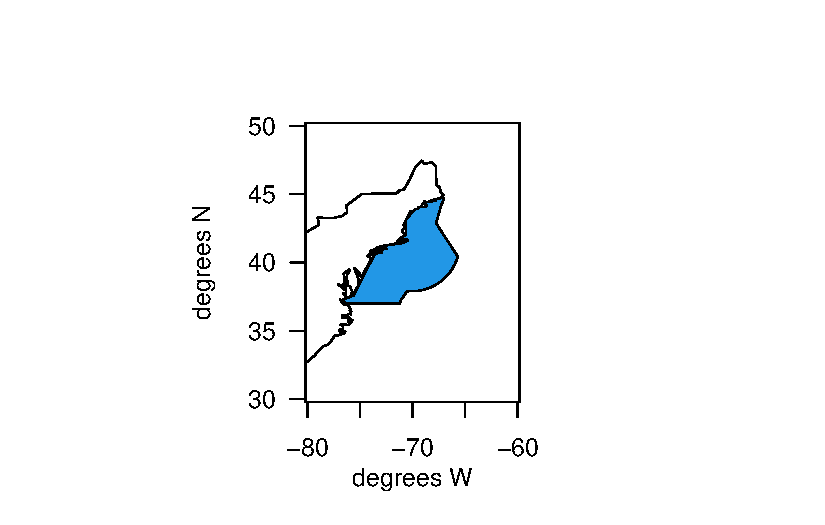
\includegraphics{makeEEZ_files/figure-pdf/unnamed-chunk-9-1.pdf}

\section{Plot all of the regions}\label{plot-all-of-the-regions}

Now we will put all of the regions on a single map and check that the
boundaries align.

\begin{Shaded}
\begin{Highlighting}[]
\FunctionTok{png}\NormalTok{(}\AttributeTok{filename =} \StringTok{"data/eez/new\_spatial\_zones1.png"}\NormalTok{, }\AttributeTok{width=} \DecValTok{800}\NormalTok{, }\AttributeTok{height =} \DecValTok{900}\NormalTok{)}

\FunctionTok{map}\NormalTok{(}\AttributeTok{database =} \StringTok{"world"}\NormalTok{, }\AttributeTok{xlim =} \FunctionTok{c}\NormalTok{(}\SpecialCharTok{{-}}\DecValTok{92}\NormalTok{, }\SpecialCharTok{{-}}\DecValTok{38}\NormalTok{), }\AttributeTok{ylim =} \FunctionTok{c}\NormalTok{(}\DecValTok{5}\NormalTok{, }\DecValTok{55}\NormalTok{), }\AttributeTok{col =} \DecValTok{8}\NormalTok{) }
\FunctionTok{mtext}\NormalTok{(}\AttributeTok{side =} \DecValTok{1}\NormalTok{, }\StringTok{"degrees W"}\NormalTok{, }\AttributeTok{line =} \DecValTok{2}\NormalTok{); }\FunctionTok{mtext}\NormalTok{(}\AttributeTok{side =} \DecValTok{2}\NormalTok{, }\StringTok{"degrees N"}\NormalTok{, }\AttributeTok{line =} \DecValTok{3}\NormalTok{)}
\FunctionTok{axis}\NormalTok{(}\DecValTok{1}\NormalTok{); }\FunctionTok{axis}\NormalTok{(}\DecValTok{2}\NormalTok{, }\AttributeTok{las =} \DecValTok{2}\NormalTok{); }\FunctionTok{box}\NormalTok{()}

\FunctionTok{polygon}\NormalTok{(CAR}\SpecialCharTok{$}\NormalTok{X, CAR}\SpecialCharTok{$}\NormalTok{Y, }\AttributeTok{border =} \DecValTok{1}\NormalTok{)}
\FunctionTok{polygon}\NormalTok{(NCA}\SpecialCharTok{$}\NormalTok{X, NCA}\SpecialCharTok{$}\NormalTok{Y, }\AttributeTok{border =} \DecValTok{1}\NormalTok{)}
\FunctionTok{polygon}\NormalTok{(NED}\SpecialCharTok{$}\NormalTok{X, NED}\SpecialCharTok{$}\NormalTok{Y, }\AttributeTok{border =} \DecValTok{1}\NormalTok{)}
\FunctionTok{polygon}\NormalTok{(FLK}\SpecialCharTok{$}\NormalTok{X, FLK}\SpecialCharTok{$}\NormalTok{Y, }\AttributeTok{border =} \DecValTok{1}\NormalTok{)}
\FunctionTok{polygon}\NormalTok{(NCFL}\SpecialCharTok{$}\NormalTok{X, NCFL}\SpecialCharTok{$}\NormalTok{Y, }\AttributeTok{border =} \DecValTok{1}\NormalTok{)}
\FunctionTok{polygon}\NormalTok{(NNC}\SpecialCharTok{$}\NormalTok{X, NNC}\SpecialCharTok{$}\NormalTok{Y, }\AttributeTok{border =} \DecValTok{1}\NormalTok{)}
\FunctionTok{polygon}\NormalTok{(VBM}\SpecialCharTok{$}\NormalTok{X, VBM}\SpecialCharTok{$}\NormalTok{Y, }\AttributeTok{border =} \DecValTok{1}\NormalTok{)}

\FunctionTok{map}\NormalTok{(}\AttributeTok{database =} \StringTok{"world"}\NormalTok{, }\AttributeTok{add =}\NormalTok{ T, }\AttributeTok{col =} \DecValTok{8}\NormalTok{, }\AttributeTok{lwd =} \DecValTok{2}\NormalTok{)}

\FunctionTok{text}\NormalTok{(}\SpecialCharTok{{-}}\DecValTok{75}\NormalTok{, }\DecValTok{15}\NormalTok{, }\StringTok{"CAR"}\NormalTok{, }\AttributeTok{cex =} \FloatTok{1.2}\NormalTok{)}
\FunctionTok{text}\NormalTok{(}\SpecialCharTok{{-}}\DecValTok{57}\NormalTok{, }\DecValTok{28}\NormalTok{, }\StringTok{"NCA"}\NormalTok{, }\AttributeTok{cex =} \FloatTok{1.2}\NormalTok{)}
\FunctionTok{text}\NormalTok{(}\SpecialCharTok{{-}}\DecValTok{57}\NormalTok{, }\DecValTok{42}\NormalTok{, }\StringTok{"NED"}\NormalTok{, }\AttributeTok{cex =} \FloatTok{1.2}\NormalTok{)}
\FunctionTok{text}\NormalTok{(}\FunctionTok{mean}\NormalTok{(FLK}\SpecialCharTok{$}\NormalTok{X), }\FunctionTok{mean}\NormalTok{(FLK}\SpecialCharTok{$}\NormalTok{Y), }\StringTok{"FLK"}\NormalTok{, }\AttributeTok{cex =} \FloatTok{1.2}\NormalTok{)}
\FunctionTok{text}\NormalTok{(}\SpecialCharTok{{-}}\FloatTok{79.3}\NormalTok{, }\FunctionTok{mean}\NormalTok{(NCFL}\SpecialCharTok{$}\NormalTok{Y), }\StringTok{"NCFL"}\NormalTok{, }\AttributeTok{cex =} \FloatTok{1.2}\NormalTok{)}
\FunctionTok{text}\NormalTok{(}\SpecialCharTok{{-}}\FloatTok{73.8}\NormalTok{, }\FunctionTok{mean}\NormalTok{(NNC}\SpecialCharTok{$}\NormalTok{Y), }\StringTok{"NNC"}\NormalTok{, }\AttributeTok{cex =} \FloatTok{1.2}\NormalTok{)}
\FunctionTok{text}\NormalTok{(}\SpecialCharTok{{-}}\FloatTok{71.5}\NormalTok{, }\FunctionTok{mean}\NormalTok{(VBM}\SpecialCharTok{$}\NormalTok{Y), }\StringTok{"VBM"}\NormalTok{, }\AttributeTok{cex =} \FloatTok{1.2}\NormalTok{)}

\FunctionTok{dev.off}\NormalTok{()}
\end{Highlighting}
\end{Shaded}

\begin{verbatim}
pdf 
  2 
\end{verbatim}

\begin{Shaded}
\begin{Highlighting}[]
\CommentTok{\#class(CAR)}

\NormalTok{CAR}\SpecialCharTok{$}\NormalTok{region }\OtherTok{\textless{}{-}} \StringTok{"CAR"}
\NormalTok{FLK}\SpecialCharTok{$}\NormalTok{region }\OtherTok{\textless{}{-}} \StringTok{"FLK"}
\NormalTok{NCFL}\SpecialCharTok{$}\NormalTok{region }\OtherTok{\textless{}{-}} \StringTok{"NCFL"}
\NormalTok{NNC}\SpecialCharTok{$}\NormalTok{region }\OtherTok{\textless{}{-}} \StringTok{"NNC"}
\NormalTok{VBM}\SpecialCharTok{$}\NormalTok{region }\OtherTok{\textless{}{-}} \StringTok{"VBM"}
\NormalTok{NCA}\SpecialCharTok{$}\NormalTok{region }\OtherTok{\textless{}{-}} \StringTok{"NCA"}
\NormalTok{NED}\SpecialCharTok{$}\NormalTok{region }\OtherTok{\textless{}{-}} \StringTok{"NED"}

\NormalTok{zones }\OtherTok{\textless{}{-}} \FunctionTok{rbind}\NormalTok{(FLK, NCFL, NNC, VBM, NED, NCA, CAR)}

\CommentTok{\# plot(zones$X, zones$Y, col = as.numeric(as.factor(zones$region)))}

\CommentTok{\# output the coordinates to a .csv file}
\FunctionTok{write.csv}\NormalTok{(zones, }\AttributeTok{file =} \StringTok{"data/eez/dolphin\_OM\_areas.csv"}\NormalTok{, }\AttributeTok{row.names =} \ConstantTok{FALSE}\NormalTok{)}
\end{Highlighting}
\end{Shaded}

\begin{figure}[H]

{\centering 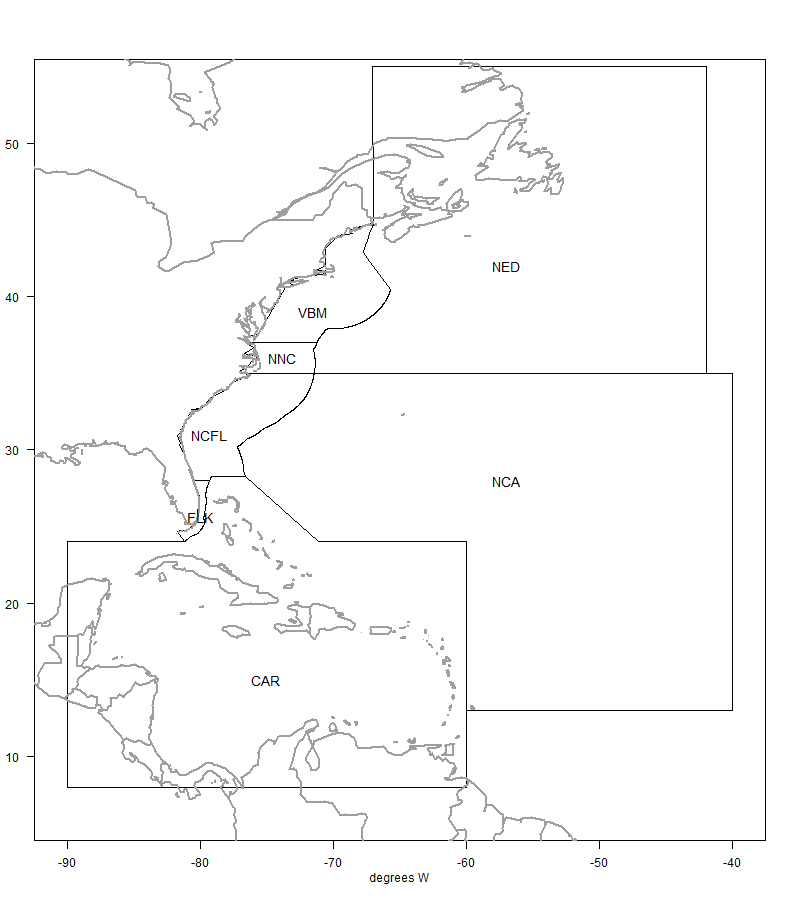
\includegraphics{data/eez/new_spatial_zones1.png}

}

\caption{Areas defined in the operating model.}

\end{figure}%

\bookmarksetup{startatroot}

\chapter{NOAA Fisheries recreational landings
data}\label{noaa-fisheries-recreational-landings-data}

Here we will partition recreational landings data from NOAA Fisheries'
Marine Recreational Information Program (MRIP), a standardized,
peer-reviewed suite of recreational fishing surveys used to produce
catch and effort estimates for quota monitoring and stock assessment in
the United States. MRIP is a standardized survey suite that employs a
complex statistical sampling design stratified across time, regions of
the coast, and different fishing modes, which allows the intercept data
to be scaled up by effort estimates to calculate total landings.

\section{Data access and upload}\label{data-access-and-upload}

Data are downloaded directly from the Miami server using the files
provided to SERO for ACL monitoring. The current location is:
M://SFD/SECM-SFD/ACL/2025\_Jun23\_MRIP\_MRFSS/. The landings are in FES
MRIP and the units are in pounds whole weight.

\begin{Shaded}
\begin{Highlighting}[]
\CommentTok{\# clear workspace}
\FunctionTok{rm}\NormalTok{(}\AttributeTok{list =} \FunctionTok{ls}\NormalTok{())}

\CommentTok{\# read in data file}
\FunctionTok{load}\NormalTok{(}\StringTok{"data/mrip\_fes\_rec81\_25wv2\_23June25.RData"}\NormalTok{)  }\CommentTok{\# most recent file on SFD server}
\FunctionTok{head}\NormalTok{(dat)}
\end{Highlighting}
\end{Shaded}

\begin{verbatim}
  REC_ACL_MRIP_FES_ID YEAR MONTH WAVE SUB_REG NEW_ST NEW_STA NEW_MODE NEW_MODEN
1            73407425 1989    NA    4       6      9      NC        4      Priv
2            73407426 1989    NA    4       6      9      NC        4      Priv
3            73407427 1989    NA    4       6      9      NC        4      Priv
4            73407428 1989    NA    4       6      9      NC        4      Priv
5            73407429 1989    NA    4       6      9      NC        4      Priv
6            73407430 1989    NA    4       6      9      NC        4      Priv
  AREA_X NEW_AREA  NEW_AREAN FL_REG NC_REG   DS               NEW_SCI
1      5        5    Inshore     NA      S MRIP Centropristis striata
2      5        5    Inshore     NA      N MRIP Centropristis striata
3      2        2  Ocean>3mi     NA      N MRIP Centropristis striata
4      2        2  Ocean>3mi     NA      S MRIP Centropristis striata
5      1        1 Ocean<=3mi     NA      N MRIP Centropristis striata
6      1        1 Ocean<=3mi     NA      S MRIP Centropristis striata
         NEW_COM    SP_CODE SPECIES_ITIS SPECIES        AB1          B2
1 black sea bass 8835020301       167687         34181.4033 121019.1368
2 black sea bass 8835020301       167687           795.8612   4445.0527
3 black sea bass 8835020301       167687           549.5390   2919.4840
4 black sea bass 8835020301       167687         71823.2390  24548.2535
5 black sea bass 8835020301       167687           415.7642     87.5928
6 black sea bass 8835020301       167687         48728.5632  11859.6428
           A         B1 LBSEST_SECWWT LBSEST_SECSOURCE SAMPLE_SIZE_USED
1 31761.4755  2419.9278    11457.8425          srysmwa               41
2   584.4155   211.4457      266.7782          srysmwa               41
3   549.5390     0.0000      484.4319          srysmwa              119
4 33343.1844 38480.0546    63313.9276          srysmwa              119
5   415.7642     0.0000      294.0623          srysmwa               71
6 40585.0152  8143.5480    34464.8156          srysmwa               71
   AVG_LEN   AVG_WGT SRYSMWA_AVG_LEN SRYSMWA_AVG_WGT SRYSMWA_SAMPLE_SIZE
1 203.4572 0.3352069        203.4572       0.3352069                  41
2 203.4572 0.3352069        203.4572       0.3352069                  41
3 296.2590 0.8815243        296.2590       0.8815243                 119
4 296.2590 0.8815243        296.2590       0.8815243                 119
5 261.9949 0.7072816        261.9949       0.7072816                  71
6 261.9949 0.7072816        261.9949       0.7072816                  71
  SRYSMWA_FLAGGED SRYSMW_AVG_LEN SRYSMW_AVG_WGT SRYSMW_SAMPLE_SIZE
1              NA       269.2563      0.7310037                231
2              NA       269.2563      0.7310037                231
3              NA       269.2563      0.7310037                231
4              NA       269.2563      0.7310037                231
5              NA       269.2563      0.7310037                231
6              NA       269.2563      0.7310037                231
  SRYSMW_FLAGGED SRYSM_AVG_LEN SRYSM_AVG_WGT SRYSM_SAMPLE_SIZE SRYSM_FLAGGED
1             NA      259.7694     0.6948228               556            NA
2             NA      259.7694     0.6948228               556            NA
3             NA      259.7694     0.6948228               556            NA
4             NA      259.7694     0.6948228               556            NA
5             NA      259.7694     0.6948228               556            NA
6             NA      259.7694     0.6948228               556            NA
  SRYS_AVG_LEN SRYS_AVG_WGT SRYS_SAMPLE_SIZE SRYS_FLAGGED SRY_AVG_LEN
1      270.955    0.8099641              982           NA    269.1276
2      270.955    0.8099641              982           NA    269.1276
3      270.955    0.8099641              982           NA    269.1276
4      270.955    0.8099641              982           NA    269.1276
5      270.955    0.8099641              982           NA    269.1276
6      270.955    0.8099641              982           NA    269.1276
  SRY_AVG_WGT SRY_SAMPLE_SIZE SRY_FLAGGED SR_AVG_LEN SR_AVG_WGT SR_SAMPLE_SIZE
1   0.8085211            1703          NA   303.6871   1.050403          46055
2   0.8085211            1703          NA   303.6871   1.050403          46055
3   0.8085211            1703          NA   303.6871   1.050403          46055
4   0.8085211            1703          NA   303.6871   1.050403          46055
5   0.8085211            1703          NA   303.6871   1.050403          46055
6   0.8085211            1703          NA   303.6871   1.050403          46055
  SR_FLAGGED S_AVG_LEN S_AVG_WGT S_SAMPLE_SIZE S_FLAGGED     VAR_B2   VAR_AB1
1         NA  344.4373  1.364082        305089        NA 4072492794 310099094
2         NA  344.4373  1.364082        305089        NA    2866289    258947
3         NA  344.4373  1.364082        305089        NA          0         0
4         NA  344.4373  1.364082        305089        NA  105731413 534702898
5         NA  344.4373  1.364082        305089        NA          0         0
6         NA  344.4373  1.364082        305089        NA   22265768 286196169
         SA_LABEL GOM_LABEL REC_ACL MIGRA_GRP AGG_MODEN JURISDICTION PS_REG
1 Snapper Grouper                 1             Private        State      6
2 Snapper Grouper                 1             Private        State      5
3 Snapper Grouper                 1             Private      Federal      5
4 Snapper Grouper                 1             Private      Federal      6
5 Snapper Grouper                 1             Private        State      5
6 Snapper Grouper                 1             Private        State      6
  COUNCILREG GFMC_FMP SAFMC_FMU LBSEST_SECGWT AGGR_AREA AREA FIRST_MONTH
1          6                  Y     9710.0360             NA          NA
2          5                  Y      226.0832             NA          NA
3          5                  Y      410.5355             NA          NA
4          6                  Y    53655.8708             NA          NA
5          5                  Y      249.2054             NA          NA
6          6                  Y    29207.4709             NA          NA
  LAST_MONTH ALT_FLAG CHTS_CL CHTS_H CHTS_RL CHTS_WAB1C CHTS_WAB1H MODE_FX
1         NA        0       0      0       0          0          0       7
2         NA        0       0      0       0          0          0       7
3         NA        0       0      0       0          0          0       7
4         NA        0       0      0       0          0          0       7
5         NA        0       0      0       0          0          0       7
6         NA        0       0      0       0          0          0       7
  NEW_SEASN SEASON
1               NA
2               NA
3               NA
4               NA
5               NA
6               NA
\end{verbatim}

\begin{Shaded}
\begin{Highlighting}[]
\CommentTok{\#apply(dat[2:18], 2, table, useNA = "always")}

\CommentTok{\# confirm nomenclature for dolphin and subset by species {-}{-}{-}{-}{-}{-}{-}{-}{-}{-}{-}{-}{-}{-}{-}{-}{-}{-}{-}{-}{-}{-}{-}{-}{-}{-}}
\FunctionTok{table}\NormalTok{(dat}\SpecialCharTok{$}\NormalTok{NEW\_COM[}\FunctionTok{grep}\NormalTok{(}\StringTok{"dolphin"}\NormalTok{, dat}\SpecialCharTok{$}\NormalTok{NEW\_COM)])}
\end{Highlighting}
\end{Shaded}

\begin{verbatim}

dolphin 
   9377 
\end{verbatim}

\begin{Shaded}
\begin{Highlighting}[]
\FunctionTok{table}\NormalTok{(dat}\SpecialCharTok{$}\NormalTok{NEW\_SCI[}\FunctionTok{grep}\NormalTok{(}\StringTok{"dolphin"}\NormalTok{, dat}\SpecialCharTok{$}\NormalTok{NEW\_COM)])}
\end{Highlighting}
\end{Shaded}

\begin{verbatim}

Coryphaena hippurus 
               9377 
\end{verbatim}

\begin{Shaded}
\begin{Highlighting}[]
\NormalTok{d }\OtherTok{\textless{}{-}}\NormalTok{ dat[}\FunctionTok{which}\NormalTok{(dat}\SpecialCharTok{$}\NormalTok{NEW\_COM }\SpecialCharTok{==} \StringTok{"dolphin"}\NormalTok{), ]}
\CommentTok{\#apply(d[2:18], 2, table, useNA = "always")}
\NormalTok{d }\OtherTok{\textless{}{-}}\NormalTok{ d[}\FunctionTok{which}\NormalTok{(d}\SpecialCharTok{$}\NormalTok{YEAR }\SpecialCharTok{\textless{}} \DecValTok{2025}\NormalTok{), ]    }\CommentTok{\# take out 2025 because incomplete year      }
\end{Highlighting}
\end{Shaded}

\section{Separate Gulf and Atlantic recreational
landings}\label{separate-gulf-and-atlantic-recreational-landings}

Now we filter the data set to separate out the Gulf versus Atlantic
landings.

\begin{Shaded}
\begin{Highlighting}[]
\CommentTok{\# codes for WFL regions: 1 (NW FL Panhandle{-} Escambia to Dixie co.), 2 (SW FL Peninsula{-} Levy to Collier co), 3 (FL Keys{-} Monroe co.)}
\CommentTok{\# subregional codes: 6 is Atlantic and 7 is Gulf}
\FunctionTok{table}\NormalTok{(d}\SpecialCharTok{$}\NormalTok{FL\_REG, d}\SpecialCharTok{$}\NormalTok{SUB\_REG, }\AttributeTok{useNA =} \StringTok{"always"}\NormalTok{)}
\end{Highlighting}
\end{Shaded}

\begin{verbatim}
      
          4    5    6    7 <NA>
  1       0    0    0  387    0
  2       0    0    0  110    0
  3       0    0    0  568    0
  4       0    0 1022    0    0
  5       0    0  312    0    0
  <NA>   96  585 3836 2426    0
\end{verbatim}

\begin{Shaded}
\begin{Highlighting}[]
\FunctionTok{unique}\NormalTok{(d}\SpecialCharTok{$}\NormalTok{NEW\_STA)}
\end{Highlighting}
\end{Shaded}

\begin{verbatim}
 [1] "NC"     "FLE"    "FLW"    "SC"     "GA"     "MS"     "AL"     "LA"    
 [9] "TX"     "FLE/GA" "RI"     "VA"     "DE"     "MD"     "NJ"     "CT"    
[17] "MA"     "NY"     "LA/MS"  "AL/FLW"
\end{verbatim}

\begin{Shaded}
\begin{Highlighting}[]
\NormalTok{lis }\OtherTok{\textless{}{-}} \FunctionTok{c}\NormalTok{(}\StringTok{"TX"}\NormalTok{, }\StringTok{"LA"}\NormalTok{, }\StringTok{"LA/MS"}\NormalTok{, }\StringTok{"MS"}\NormalTok{, }\StringTok{"AL"}\NormalTok{, }\StringTok{"AL/FLW"}\NormalTok{)  }\CommentTok{\# filter out the Gulf states}
\NormalTok{d1 }\OtherTok{\textless{}{-}}\NormalTok{ d[}\SpecialCharTok{{-}}\FunctionTok{which}\NormalTok{(d}\SpecialCharTok{$}\NormalTok{NEW\_STA }\SpecialCharTok{\%in\%}\NormalTok{ lis), ]}
\FunctionTok{unique}\NormalTok{(d1}\SpecialCharTok{$}\NormalTok{NEW\_STA)}
\end{Highlighting}
\end{Shaded}

\begin{verbatim}
 [1] "NC"     "FLE"    "FLW"    "SC"     "GA"     "FLE/GA" "RI"     "VA"    
 [9] "DE"     "MD"     "NJ"     "CT"     "MA"     "NY"    
\end{verbatim}

\begin{Shaded}
\begin{Highlighting}[]
\FunctionTok{table}\NormalTok{(d1}\SpecialCharTok{$}\NormalTok{FL\_REG, d1}\SpecialCharTok{$}\NormalTok{NEW\_STA, }\AttributeTok{useNA =} \StringTok{"always"}\NormalTok{)  }
\end{Highlighting}
\end{Shaded}

\begin{verbatim}
      
         CT   DE  FLE FLE/GA  FLW   GA   MA   MD   NC   NJ   NY   RI   SC   VA
  1       0    0    0      0  387    0    0    0    0    0    0    0    0    0
  2       0    0    0      0  110    0    0    0    0    0    0    0    0    0
  3       0    0    0      0  568    0    0    0    0    0    0    0    0    0
  4       0    0 1022      0    0    0    0    0    0    0    0    0    0    0
  5       0    0  312      0    0    0    0    0    0    0    0    0    0    0
  <NA>   14  114    0   1794  174   54   20  125 1344  108   73   62  644  165
      
       <NA>
  1       0
  2       0
  3       0
  4       0
  5       0
  <NA>    0
\end{verbatim}

\begin{Shaded}
\begin{Highlighting}[]
\FunctionTok{dim}\NormalTok{(d1)}
\end{Highlighting}
\end{Shaded}

\begin{verbatim}
[1] 7090   83
\end{verbatim}

\begin{Shaded}
\begin{Highlighting}[]
\NormalTok{d1 }\OtherTok{\textless{}{-}}\NormalTok{ d1[}\SpecialCharTok{{-}}\FunctionTok{which}\NormalTok{(d1}\SpecialCharTok{$}\NormalTok{FL\_REG }\SpecialCharTok{==} \DecValTok{1} \SpecialCharTok{|}\NormalTok{ d1}\SpecialCharTok{$}\NormalTok{FL\_REG }\SpecialCharTok{==} \DecValTok{2}\NormalTok{), ]   }\CommentTok{\# filter out FL regions 1 and 2 but retain 3 (FL Keys)}
\FunctionTok{dim}\NormalTok{(d1)}
\end{Highlighting}
\end{Shaded}

\begin{verbatim}
[1] 6593   83
\end{verbatim}

\begin{Shaded}
\begin{Highlighting}[]
\NormalTok{d1 }\OtherTok{\textless{}{-}}\NormalTok{ d1[}\SpecialCharTok{{-}}\FunctionTok{which}\NormalTok{(}\FunctionTok{is.na}\NormalTok{(d1}\SpecialCharTok{$}\NormalTok{FL\_REG) }\SpecialCharTok{\&}\NormalTok{ d1}\SpecialCharTok{$}\NormalTok{NEW\_STA }\SpecialCharTok{==} \StringTok{"FLW"}\NormalTok{), ]  }\CommentTok{\# filter out FLW with unknown FL region}
\FunctionTok{dim}\NormalTok{(d1)}
\end{Highlighting}
\end{Shaded}

\begin{verbatim}
[1] 6419   83
\end{verbatim}

\begin{Shaded}
\begin{Highlighting}[]
\FunctionTok{table}\NormalTok{(d1}\SpecialCharTok{$}\NormalTok{FL\_REG, d1}\SpecialCharTok{$}\NormalTok{NEW\_STA, }\AttributeTok{useNA =} \StringTok{"always"}\NormalTok{)  }\CommentTok{\# retained are all Atlantic states plus region 3 of Florida}
\end{Highlighting}
\end{Shaded}

\begin{verbatim}
      
         CT   DE  FLE FLE/GA  FLW   GA   MA   MD   NC   NJ   NY   RI   SC   VA
  3       0    0    0      0  568    0    0    0    0    0    0    0    0    0
  4       0    0 1022      0    0    0    0    0    0    0    0    0    0    0
  5       0    0  312      0    0    0    0    0    0    0    0    0    0    0
  <NA>   14  114    0   1794    0   54   20  125 1344  108   73   62  644  165
      
       <NA>
  3       0
  4       0
  5       0
  <NA>    0
\end{verbatim}

Now we can summarize the total dolphin landings in weight for the U.S.
Atlantic, and compare to previous values sent for quota monitoring. We
see that the values are almost identical.

\begin{Shaded}
\begin{Highlighting}[]
\CommentTok{\# summarize by year and compare {-}{-}{-}{-}{-}{-}{-}{-}{-}{-}{-}{-}{-}{-}{-}{-}{-}{-}{-}{-}{-}{-}{-}{-}{-}{-}}

\NormalTok{tot1 }\OtherTok{\textless{}{-}} \FunctionTok{tapply}\NormalTok{(d1}\SpecialCharTok{$}\NormalTok{LBSEST\_SECWWT, d1}\SpecialCharTok{$}\NormalTok{YEAR, sum, }\AttributeTok{na.rm =}\NormalTok{ T)}
\CommentTok{\#head(tot1)}

\NormalTok{old }\OtherTok{\textless{}{-}} \FunctionTok{read.csv}\NormalTok{(}\StringTok{"data/RecreationalDolphinLandings\_SAandGOM\_MLarkin.csv"}\NormalTok{, }\AttributeTok{skip =} \DecValTok{6}\NormalTok{)}
\FunctionTok{plot}\NormalTok{(old}\SpecialCharTok{$}\NormalTok{Year, old}\SpecialCharTok{$}\NormalTok{ATL, }\AttributeTok{type =} \StringTok{"l"}\NormalTok{, }\AttributeTok{xlab =} \StringTok{"year"}\NormalTok{, }\AttributeTok{ylab =} \StringTok{"total catch (pounds)"}\NormalTok{, }\AttributeTok{lwd =} \DecValTok{4}\NormalTok{, }
     \AttributeTok{xlim =} \FunctionTok{c}\NormalTok{(}\DecValTok{1980}\NormalTok{, }\DecValTok{2025}\NormalTok{), }\AttributeTok{ylim =} \FunctionTok{c}\NormalTok{(}\DecValTok{7}\SpecialCharTok{*}\DecValTok{10}\SpecialCharTok{\^{}}\DecValTok{6}\NormalTok{, }\FloatTok{3.3}\SpecialCharTok{*}\DecValTok{10}\SpecialCharTok{\^{}}\DecValTok{7}\NormalTok{), }\AttributeTok{bty =} \StringTok{"n"}\NormalTok{)}
\FunctionTok{lines}\NormalTok{(}\FunctionTok{as.numeric}\NormalTok{(}\FunctionTok{names}\NormalTok{(tot1)), tot1, }\AttributeTok{lwd =} \DecValTok{2}\NormalTok{, }\AttributeTok{col =} \DecValTok{2}\NormalTok{, }\AttributeTok{lty =} \DecValTok{2}\NormalTok{)}
\FunctionTok{legend}\NormalTok{(}\StringTok{"topright"}\NormalTok{, }\FunctionTok{c}\NormalTok{(}\StringTok{"previous data"}\NormalTok{, }\StringTok{"new data"}\NormalTok{), }\AttributeTok{col =} \FunctionTok{c}\NormalTok{(}\DecValTok{1}\NormalTok{, }\DecValTok{2}\NormalTok{), }\AttributeTok{lwd =} \FunctionTok{c}\NormalTok{(}\DecValTok{4}\NormalTok{, }\DecValTok{2}\NormalTok{), }\AttributeTok{lty =} \FunctionTok{c}\NormalTok{(}\DecValTok{1}\NormalTok{, }\DecValTok{2}\NormalTok{))}
\end{Highlighting}
\end{Shaded}

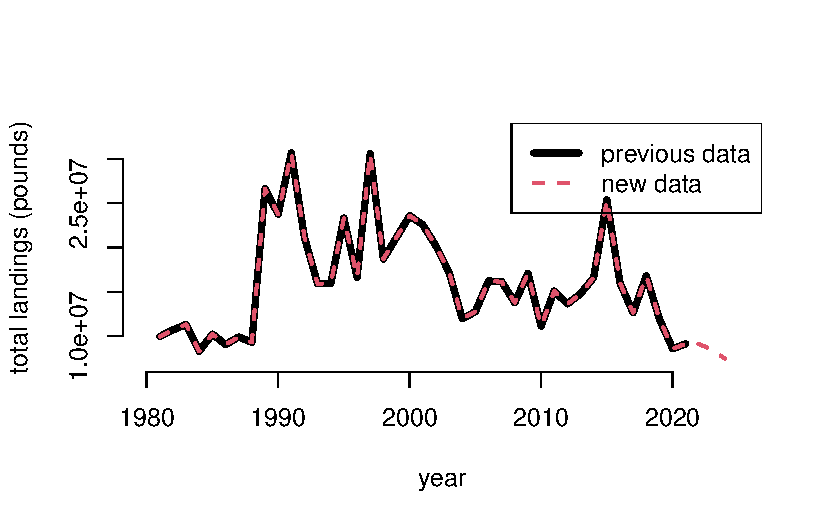
\includegraphics{MRIP_files/figure-pdf/unnamed-chunk-3-1.pdf}

\section{Partition catches by area and
sector}\label{partition-catches-by-area-and-sector}

Now we will partition out the total catches according to the dolphin MSE
areas. The areas are as follows:

\begin{itemize}
\tightlist
\item
  FLK: Florida Keys to Indian River County County (FL)
\item
  NCFL: Brevard (FL) to Southern NC (South of Hatteras)
\item
  NNC: Northern NC (North of Hatteras to NC/VA border)
\item
  VBM: Virginia to Maine
\end{itemize}

\begin{Shaded}
\begin{Highlighting}[]
\CommentTok{\# separate out 4 regions {-}{-}{-}{-}{-}{-}{-}{-}{-}{-}{-}{-}{-}{-}{-}{-}{-}{-}{-}{-}{-}{-}{-}{-}{-}{-}}

\NormalTok{d1}\SpecialCharTok{$}\NormalTok{region }\OtherTok{\textless{}{-}} \StringTok{"VBM"}

\CommentTok{\# select for FLK}
\CommentTok{\# FL\_REG codes: 4: SE FL{-} Miami{-}Dade to Indian River County.; 5: NE FL{-} Brevard to Nassau County}
\FunctionTok{table}\NormalTok{(d1}\SpecialCharTok{$}\NormalTok{FL\_REG, d1}\SpecialCharTok{$}\NormalTok{NEW\_STA, }\AttributeTok{useNA =} \StringTok{"always"}\NormalTok{)}
\end{Highlighting}
\end{Shaded}

\begin{verbatim}
      
         CT   DE  FLE FLE/GA  FLW   GA   MA   MD   NC   NJ   NY   RI   SC   VA
  3       0    0    0      0  568    0    0    0    0    0    0    0    0    0
  4       0    0 1022      0    0    0    0    0    0    0    0    0    0    0
  5       0    0  312      0    0    0    0    0    0    0    0    0    0    0
  <NA>   14  114    0   1794    0   54   20  125 1344  108   73   62  644  165
      
       <NA>
  3       0
  4       0
  5       0
  <NA>    0
\end{verbatim}

\begin{Shaded}
\begin{Highlighting}[]
\NormalTok{d1}\SpecialCharTok{$}\NormalTok{region[}\FunctionTok{which}\NormalTok{(d1}\SpecialCharTok{$}\NormalTok{FL\_REG }\SpecialCharTok{==} \DecValTok{3} \SpecialCharTok{|}\NormalTok{ d1}\SpecialCharTok{$}\NormalTok{FL\_REG }\SpecialCharTok{==} \DecValTok{4}\NormalTok{)] }\OtherTok{\textless{}{-}} \StringTok{"FLK"}

\CommentTok{\# select for NCFL}
\NormalTok{d1}\SpecialCharTok{$}\NormalTok{region[}\FunctionTok{which}\NormalTok{(d1}\SpecialCharTok{$}\NormalTok{FL\_REG }\SpecialCharTok{==} \DecValTok{5}\NormalTok{)] }\OtherTok{\textless{}{-}} \StringTok{"NCFL"}
\NormalTok{lis }\OtherTok{\textless{}{-}} \FunctionTok{c}\NormalTok{(}\StringTok{"SC"}\NormalTok{, }\StringTok{"GA"}\NormalTok{, }\StringTok{"FLE/GA"}\NormalTok{)           }\CommentTok{\# NCFL states}
\NormalTok{d1}\SpecialCharTok{$}\NormalTok{region[}\FunctionTok{which}\NormalTok{(d1}\SpecialCharTok{$}\NormalTok{NEW\_STA }\SpecialCharTok{\%in\%}\NormalTok{ lis)] }\OtherTok{\textless{}{-}} \StringTok{"NCFL"}
\CommentTok{\# NC\_REG codes: N: North of Cape Hatteras; S: South of Cape Hatteras}
\FunctionTok{table}\NormalTok{(d1}\SpecialCharTok{$}\NormalTok{NC\_REG, d1}\SpecialCharTok{$}\NormalTok{NEW\_STA, }\AttributeTok{useNA =} \StringTok{"always"}\NormalTok{)}
\end{Highlighting}
\end{Shaded}

\begin{verbatim}
      
         CT   DE  FLE FLE/GA  FLW   GA   MA   MD   NC   NJ   NY   RI   SC   VA
         14  114 1334   1794  568   54   20  125  586  108   73   62  644  165
  N       0    0    0      0    0    0    0    0  420    0    0    0    0    0
  S       0    0    0      0    0    0    0    0  338    0    0    0    0    0
  <NA>    0    0    0      0    0    0    0    0    0    0    0    0    0    0
      
       <NA>
          0
  N       0
  S       0
  <NA>    0
\end{verbatim}

\begin{Shaded}
\begin{Highlighting}[]
\NormalTok{d1}\SpecialCharTok{$}\NormalTok{region[}\FunctionTok{which}\NormalTok{(d1}\SpecialCharTok{$}\NormalTok{NC }\SpecialCharTok{==} \StringTok{"S"}\NormalTok{)] }\OtherTok{\textless{}{-}} \StringTok{"NCFL"}

\CommentTok{\# select for NNC}
\NormalTok{d1}\SpecialCharTok{$}\NormalTok{region[}\FunctionTok{which}\NormalTok{(d1}\SpecialCharTok{$}\NormalTok{NC }\SpecialCharTok{==} \StringTok{"N"}\NormalTok{)] }\OtherTok{\textless{}{-}} \StringTok{"NNC"}

\FunctionTok{table}\NormalTok{(d1}\SpecialCharTok{$}\NormalTok{FL\_REG, d1}\SpecialCharTok{$}\NormalTok{NEW\_STA, d1}\SpecialCharTok{$}\NormalTok{region)}
\end{Highlighting}
\end{Shaded}

\begin{verbatim}
, ,  = FLK

   
      CT   DE  FLE FLE/GA  FLW   GA   MA   MD   NC   NJ   NY   RI   SC   VA
  3    0    0    0      0  568    0    0    0    0    0    0    0    0    0
  4    0    0 1022      0    0    0    0    0    0    0    0    0    0    0
  5    0    0    0      0    0    0    0    0    0    0    0    0    0    0

, ,  = NCFL

   
      CT   DE  FLE FLE/GA  FLW   GA   MA   MD   NC   NJ   NY   RI   SC   VA
  3    0    0    0      0    0    0    0    0    0    0    0    0    0    0
  4    0    0    0      0    0    0    0    0    0    0    0    0    0    0
  5    0    0  312      0    0    0    0    0    0    0    0    0    0    0

, ,  = NNC

   
      CT   DE  FLE FLE/GA  FLW   GA   MA   MD   NC   NJ   NY   RI   SC   VA
  3    0    0    0      0    0    0    0    0    0    0    0    0    0    0
  4    0    0    0      0    0    0    0    0    0    0    0    0    0    0
  5    0    0    0      0    0    0    0    0    0    0    0    0    0    0

, ,  = VBM

   
      CT   DE  FLE FLE/GA  FLW   GA   MA   MD   NC   NJ   NY   RI   SC   VA
  3    0    0    0      0    0    0    0    0    0    0    0    0    0    0
  4    0    0    0      0    0    0    0    0    0    0    0    0    0    0
  5    0    0    0      0    0    0    0    0    0    0    0    0    0    0
\end{verbatim}

\begin{Shaded}
\begin{Highlighting}[]
\FunctionTok{table}\NormalTok{(d1}\SpecialCharTok{$}\NormalTok{NC\_REG, d1}\SpecialCharTok{$}\NormalTok{NEW\_STA, d1}\SpecialCharTok{$}\NormalTok{region)  }\CommentTok{\# check classification}
\end{Highlighting}
\end{Shaded}

\begin{verbatim}
, ,  = FLK

   
      CT   DE  FLE FLE/GA  FLW   GA   MA   MD   NC   NJ   NY   RI   SC   VA
       0    0 1022      0  568    0    0    0    0    0    0    0    0    0
  N    0    0    0      0    0    0    0    0    0    0    0    0    0    0
  S    0    0    0      0    0    0    0    0    0    0    0    0    0    0

, ,  = NCFL

   
      CT   DE  FLE FLE/GA  FLW   GA   MA   MD   NC   NJ   NY   RI   SC   VA
       0    0  312   1794    0   54    0    0    0    0    0    0  644    0
  N    0    0    0      0    0    0    0    0    0    0    0    0    0    0
  S    0    0    0      0    0    0    0    0  338    0    0    0    0    0

, ,  = NNC

   
      CT   DE  FLE FLE/GA  FLW   GA   MA   MD   NC   NJ   NY   RI   SC   VA
       0    0    0      0    0    0    0    0    0    0    0    0    0    0
  N    0    0    0      0    0    0    0    0  420    0    0    0    0    0
  S    0    0    0      0    0    0    0    0    0    0    0    0    0    0

, ,  = VBM

   
      CT   DE  FLE FLE/GA  FLW   GA   MA   MD   NC   NJ   NY   RI   SC   VA
      14  114    0      0    0    0   20  125  586  108   73   62    0  165
  N    0    0    0      0    0    0    0    0    0    0    0    0    0    0
  S    0    0    0      0    0    0    0    0    0    0    0    0    0    0
\end{verbatim}

Now we will separate out the catches by recreational sector and plot the
totals by region and sector.

\begin{Shaded}
\begin{Highlighting}[]
\CommentTok{\# separate out by for hire vs. private rec {-}{-}{-}{-}{-}{-}{-}{-}{-}{-}{-}{-}{-}{-}{-}{-}{-}{-}{-}{-}{-}{-}{-}{-}{-}{-}}
\NormalTok{d1}\SpecialCharTok{$}\NormalTok{sector }\OtherTok{\textless{}{-}} \StringTok{"ForHire"}

\NormalTok{d1}\SpecialCharTok{$}\NormalTok{sector[}\FunctionTok{which}\NormalTok{(d1}\SpecialCharTok{$}\NormalTok{NEW\_MODEN }\SpecialCharTok{==} \StringTok{"Shore"}\NormalTok{)] }\OtherTok{\textless{}{-}} \StringTok{"Rec"}
\NormalTok{d1}\SpecialCharTok{$}\NormalTok{sector[}\FunctionTok{which}\NormalTok{(d1}\SpecialCharTok{$}\NormalTok{NEW\_MODEN }\SpecialCharTok{==} \StringTok{"Priv"}\NormalTok{)]  }\OtherTok{\textless{}{-}} \StringTok{"Rec"}

\FunctionTok{table}\NormalTok{(d1}\SpecialCharTok{$}\NormalTok{sector, d1}\SpecialCharTok{$}\NormalTok{NEW\_MODEN, }\AttributeTok{useNA =} \StringTok{"always"}\NormalTok{)    }\CommentTok{\# check classification}
\end{Highlighting}
\end{Shaded}

\begin{verbatim}
         
           Cbt Cbt/Hbt  Hbt Priv Shore <NA>
  ForHire 1616     119 2912    0     0    0
  Rec        0       0    0 1750    22    0
  <NA>       0       0    0    0     0    0
\end{verbatim}

\begin{Shaded}
\begin{Highlighting}[]
\NormalTok{tot }\OtherTok{\textless{}{-}} \FunctionTok{tapply}\NormalTok{(d1}\SpecialCharTok{$}\NormalTok{LBSEST\_SECWWT, }\FunctionTok{list}\NormalTok{(d1}\SpecialCharTok{$}\NormalTok{YEAR, d1}\SpecialCharTok{$}\NormalTok{region, d1}\SpecialCharTok{$}\NormalTok{sector), sum, }\AttributeTok{na.rm =}\NormalTok{ T)}

\FunctionTok{head}\NormalTok{(tot)}
\end{Highlighting}
\end{Shaded}

\begin{verbatim}
, , ForHire

           FLK      NCFL       NNC       VBM
1981  354639.5  74702.50 256755.24  1400.247
1982  347458.2  92271.42  27578.44  2749.224
1983 1020005.8  41784.04  88690.53  5379.177
1984 1021086.8  74658.81        NA  4203.048
1985  717523.0 172989.65  58514.13  8880.857
1986 1562354.0  63555.89 817192.26 61658.193

, , Rec

          FLK      NCFL       NNC        VBM
1981  8942641  322505.7        NA         NA
1982  8422673 1711834.7 78367.161  18727.290
1983 10000662  119370.4 44226.032   5456.237
1984  6717044  486079.7        NA      0.000
1985  7925301 1162708.4 77477.096 112944.274
1986  5699311  736872.0  2549.586 103945.134
\end{verbatim}

\begin{Shaded}
\begin{Highlighting}[]
\NormalTok{fin }\OtherTok{\textless{}{-}} \FunctionTok{data.frame}\NormalTok{(}\FunctionTok{cbind}\NormalTok{(tot[, , }\DecValTok{1}\NormalTok{], tot[, , }\DecValTok{2}\NormalTok{]))}
\FunctionTok{names}\NormalTok{(fin) }\OtherTok{\textless{}{-}} \FunctionTok{c}\NormalTok{(}\StringTok{"Hire\_FLK"}\NormalTok{, }\StringTok{"Hire\_NCFL"}\NormalTok{, }\StringTok{"Hire\_NNC"}\NormalTok{, }\StringTok{"Hire\_VBM"}\NormalTok{, }
                \StringTok{"Rec\_FLK"}\NormalTok{, }\StringTok{"Rec\_NCFL"}\NormalTok{, }\StringTok{"Rec\_NNC"}\NormalTok{, }\StringTok{"Rec\_VBM"}\NormalTok{)}
\FunctionTok{head}\NormalTok{(fin)}
\end{Highlighting}
\end{Shaded}

\begin{verbatim}
      Hire_FLK Hire_NCFL  Hire_NNC  Hire_VBM  Rec_FLK  Rec_NCFL   Rec_NNC
1981  354639.5  74702.50 256755.24  1400.247  8942641  322505.7        NA
1982  347458.2  92271.42  27578.44  2749.224  8422673 1711834.7 78367.161
1983 1020005.8  41784.04  88690.53  5379.177 10000662  119370.4 44226.032
1984 1021086.8  74658.81        NA  4203.048  6717044  486079.7        NA
1985  717523.0 172989.65  58514.13  8880.857  7925301 1162708.4 77477.096
1986 1562354.0  63555.89 817192.26 61658.193  5699311  736872.0  2549.586
        Rec_VBM
1981         NA
1982  18727.290
1983   5456.237
1984      0.000
1985 112944.274
1986 103945.134
\end{verbatim}

\begin{Shaded}
\begin{Highlighting}[]
\FunctionTok{matplot}\NormalTok{(}\FunctionTok{rownames}\NormalTok{(fin), fin}\SpecialCharTok{/}\DecValTok{10}\SpecialCharTok{\^{}}\DecValTok{6}\NormalTok{, }\AttributeTok{lty =} \FunctionTok{c}\NormalTok{(}\FunctionTok{rep}\NormalTok{(}\DecValTok{2}\NormalTok{, }\DecValTok{4}\NormalTok{), }\FunctionTok{rep}\NormalTok{(}\DecValTok{1}\NormalTok{, }\DecValTok{4}\NormalTok{)), }
        \AttributeTok{col =} \FunctionTok{rep}\NormalTok{(}\DecValTok{1}\SpecialCharTok{:}\DecValTok{4}\NormalTok{, }\DecValTok{2}\NormalTok{), }\AttributeTok{type =} \StringTok{"l"}\NormalTok{, }\AttributeTok{lwd =} \DecValTok{2}\NormalTok{, }
        \AttributeTok{xlab =} \StringTok{"year"}\NormalTok{, }\AttributeTok{ylab =} \StringTok{"total catch (millions of pounds)"}\NormalTok{)}
\FunctionTok{legend}\NormalTok{(}\StringTok{"topright"}\NormalTok{, }\FunctionTok{colnames}\NormalTok{(fin), }\AttributeTok{lty =} \FunctionTok{c}\NormalTok{(}\FunctionTok{rep}\NormalTok{(}\DecValTok{2}\NormalTok{, }\DecValTok{4}\NormalTok{), }\FunctionTok{rep}\NormalTok{(}\DecValTok{1}\NormalTok{, }\DecValTok{4}\NormalTok{)), }\AttributeTok{col =} \FunctionTok{rep}\NormalTok{(}\DecValTok{1}\SpecialCharTok{:}\DecValTok{4}\NormalTok{, }\DecValTok{2}\NormalTok{), }\AttributeTok{lwd =} \DecValTok{2}\NormalTok{, }\AttributeTok{ncol =} \DecValTok{2}\NormalTok{, }\AttributeTok{bty =} \StringTok{"n"}\NormalTok{)}
\end{Highlighting}
\end{Shaded}

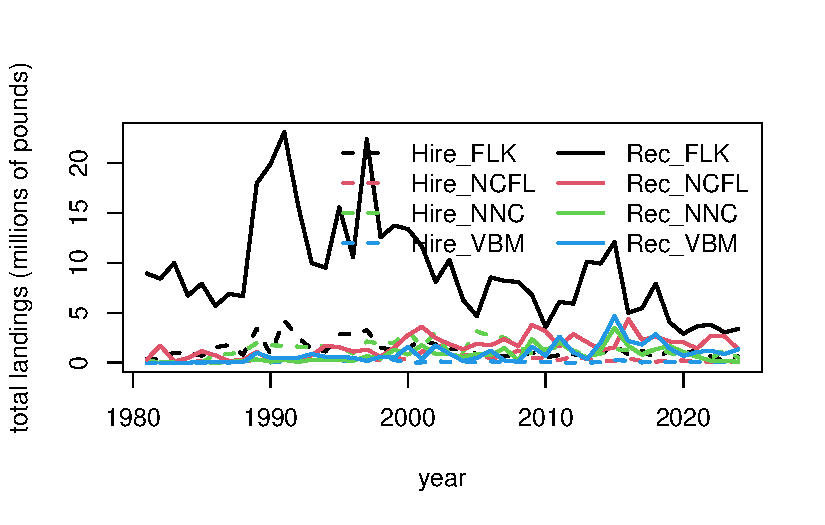
\includegraphics{MRIP_files/figure-pdf/unnamed-chunk-5-1.pdf}

\begin{Shaded}
\begin{Highlighting}[]
\CommentTok{\# check that totals match}
\FunctionTok{cor}\NormalTok{(}\FunctionTok{rowSums}\NormalTok{(fin, }\AttributeTok{na.rm =}\NormalTok{ T), tot1)}
\end{Highlighting}
\end{Shaded}

\begin{verbatim}
[1] 1
\end{verbatim}

\begin{Shaded}
\begin{Highlighting}[]
\FunctionTok{mean}\NormalTok{(}\FunctionTok{rowSums}\NormalTok{(fin, }\AttributeTok{na.rm =}\NormalTok{ T) }\SpecialCharTok{{-}}\NormalTok{ tot1)   }\CommentTok{\# very tiny differences}
\end{Highlighting}
\end{Shaded}

\begin{verbatim}
[1] 4.233284e-11
\end{verbatim}

Here are the catches (in pounds) for years 1981 to 2024.

\section{Looking at extent of
discarding}\label{looking-at-extent-of-discarding}

Discard estimates (known as B2 estimates) are provided in numbers by the
MRIP survey but are not available in the Southeast Region Headboat
Survey. We can look at the overall numbers of dolphinfish caught versus
reported released from the MRIP survey to get an understanding of the
extent of discarding.

\begin{Shaded}
\begin{Highlighting}[]
\NormalTok{d1}\SpecialCharTok{$}\NormalTok{perdis }\OtherTok{\textless{}{-}}\NormalTok{ d1}\SpecialCharTok{$}\NormalTok{B2 }\SpecialCharTok{/}\NormalTok{ (d1}\SpecialCharTok{$}\NormalTok{AB1 }\SpecialCharTok{+}\NormalTok{ d1}\SpecialCharTok{$}\NormalTok{B2)  }\CommentTok{\# percent discarded is B2 (fish released alive) / total}

\CommentTok{\# calculate mean discard rate by year, region, sector {-}{-}{-}{-}{-}{-}{-}{-}{-}{-}{-}{-}{-}{-}{-}{-}}
\NormalTok{dis }\OtherTok{\textless{}{-}} \FunctionTok{tapply}\NormalTok{(d1}\SpecialCharTok{$}\NormalTok{perdis, }\FunctionTok{list}\NormalTok{(d1}\SpecialCharTok{$}\NormalTok{YEAR, d1}\SpecialCharTok{$}\NormalTok{region, d1}\SpecialCharTok{$}\NormalTok{sector), mean, }\AttributeTok{na.rm =}\NormalTok{ T)}
\NormalTok{disr }\OtherTok{\textless{}{-}} \FunctionTok{tapply}\NormalTok{(d1}\SpecialCharTok{$}\NormalTok{perdis, }\FunctionTok{list}\NormalTok{(d1}\SpecialCharTok{$}\NormalTok{region, d1}\SpecialCharTok{$}\NormalTok{sector), mean, }\AttributeTok{na.rm =}\NormalTok{ T)}

\FunctionTok{matplot}\NormalTok{(}\FunctionTok{rownames}\NormalTok{(dis), }\FunctionTok{cbind}\NormalTok{(dis[, , }\DecValTok{1}\NormalTok{], dis[, , }\DecValTok{2}\NormalTok{]), }\AttributeTok{lty =} \FunctionTok{c}\NormalTok{(}\FunctionTok{rep}\NormalTok{(}\DecValTok{2}\NormalTok{, }\DecValTok{4}\NormalTok{), }\FunctionTok{rep}\NormalTok{(}\DecValTok{1}\NormalTok{, }\DecValTok{4}\NormalTok{)), }\AttributeTok{col =} \FunctionTok{rep}\NormalTok{(}\DecValTok{1}\SpecialCharTok{:}\DecValTok{4}\NormalTok{, }\DecValTok{2}\NormalTok{), }
        \AttributeTok{type =} \StringTok{"l"}\NormalTok{, }\AttributeTok{lwd =} \DecValTok{2}\NormalTok{, }\AttributeTok{xlab =} \StringTok{"year"}\NormalTok{, }\AttributeTok{ylab =} \StringTok{"proportion dolphin discarded alive"}\NormalTok{, }\AttributeTok{ylim =} \FunctionTok{c}\NormalTok{(}\DecValTok{0}\NormalTok{, }\FloatTok{0.5}\NormalTok{))}
\FunctionTok{legend}\NormalTok{(}\StringTok{"top"}\NormalTok{, }\FunctionTok{c}\NormalTok{(}\FunctionTok{paste}\NormalTok{(}\StringTok{"For hire {-} "}\NormalTok{, }\FunctionTok{colnames}\NormalTok{(dis)), }\FunctionTok{paste}\NormalTok{(}\StringTok{"Private {-} "}\NormalTok{, }\FunctionTok{colnames}\NormalTok{(dis))), }
       \AttributeTok{lty =} \FunctionTok{c}\NormalTok{(}\FunctionTok{rep}\NormalTok{(}\DecValTok{2}\NormalTok{, }\DecValTok{4}\NormalTok{), }\FunctionTok{rep}\NormalTok{(}\DecValTok{1}\NormalTok{, }\DecValTok{4}\NormalTok{)), }\AttributeTok{col =} \FunctionTok{rep}\NormalTok{(}\DecValTok{1}\SpecialCharTok{:}\DecValTok{4}\NormalTok{, }\DecValTok{2}\NormalTok{), }\AttributeTok{lwd =} \DecValTok{2}\NormalTok{, }\AttributeTok{ncol =} \DecValTok{2}\NormalTok{, }\AttributeTok{bty =} \StringTok{"n"}\NormalTok{)}
\end{Highlighting}
\end{Shaded}

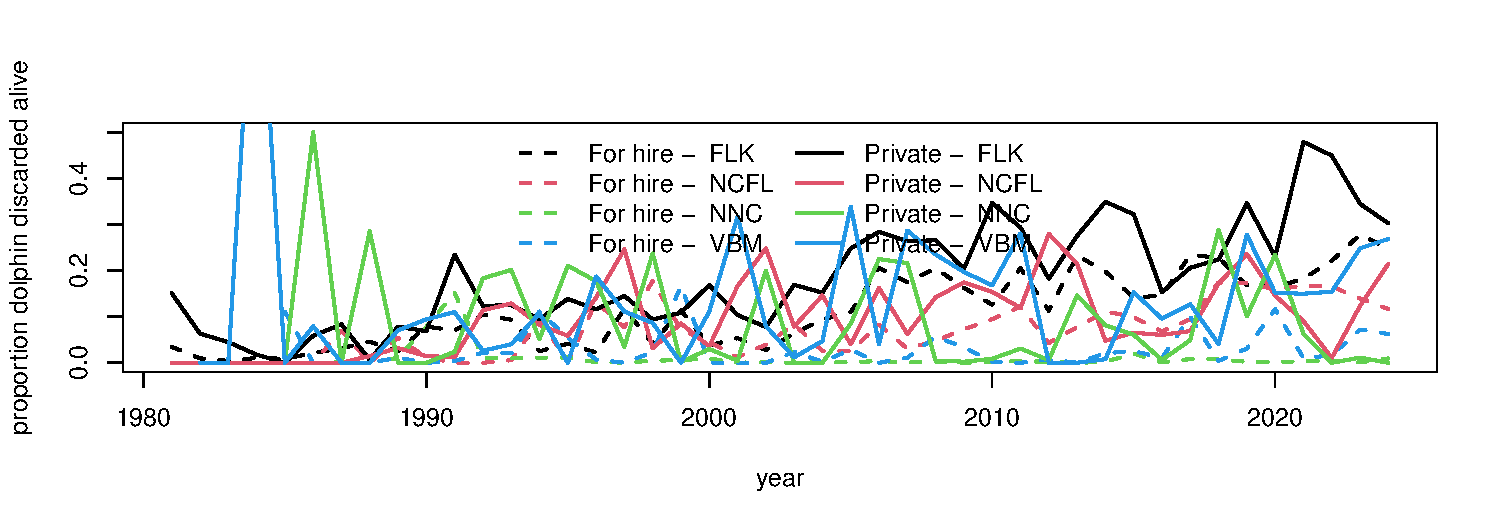
\includegraphics{MRIP_files/figure-pdf/unnamed-chunk-6-1.pdf}

\begin{Shaded}
\begin{Highlighting}[]
\FunctionTok{round}\NormalTok{(disr }\SpecialCharTok{*} \DecValTok{100}\NormalTok{, }\DecValTok{2}\NormalTok{)  }\CommentTok{\# discarding rates by region and sector}
\end{Highlighting}
\end{Shaded}

\begin{verbatim}
     ForHire   Rec
FLK    10.79 18.76
NCFL    9.44 11.23
NNC     0.94  9.62
VBM     2.94 12.69
\end{verbatim}

According to the MRIP survey and the reported numbers, discarding
generally increases over time, excluding some highly anomalous estimates
from the early years which are driven by low sample sizes. Discarding is
generally higher in the private sector compared to the for-hire sector,
and is highest in the Florida Keys region.

\section{Split the catches by season}\label{split-the-catches-by-season}

The dolphin MSE operates on a seasonal time step and thus the catches
and discards must by parsed apart by individual season and year. This is
not straightforward because MRIP estimates are reported in two-month
waves (Jan - Feb, Mar - Apr, May - Jun, etc.), and the seasons are
3-month periods (Dec - Feb, Mar - May, Jun - Aug, Sep - Nov). For the
two waves that have to be split into seasons (e.g., December is lumped
with January and February; June is lumped with July and August), we
split the wave 50/50\%, i.e, we make the assumption that half of the
catch in that wave occurs in one season and the other half occurs in the
next season.

\begin{Shaded}
\begin{Highlighting}[]
\CommentTok{\# define seasons {-}{-}{-}{-}{-}{-}{-}{-}{-}{-}{-}{-}{-}{-}{-}{-}{-}{-}{-}{-}{-}{-}{-}{-}{-}{-}{-}{-}{-}}
\FunctionTok{table}\NormalTok{(d1}\SpecialCharTok{$}\NormalTok{WAVE, }\AttributeTok{useNA =} \StringTok{"always"}\NormalTok{)}
\end{Highlighting}
\end{Shaded}

\begin{verbatim}

   0    1    2    3    4    5    6 <NA> 
   5  407  718 1230 1439 1095  581  944 
\end{verbatim}

\begin{Shaded}
\begin{Highlighting}[]
\NormalTok{d1}\SpecialCharTok{$}\NormalTok{YRWAVE }\OtherTok{\textless{}{-}} \FunctionTok{paste0}\NormalTok{(d1}\SpecialCharTok{$}\NormalTok{YEAR, }\StringTok{"\_"}\NormalTok{, d1}\SpecialCharTok{$}\NormalTok{WAVE)}

\NormalTok{totw }\OtherTok{\textless{}{-}} \FunctionTok{tapply}\NormalTok{(d1}\SpecialCharTok{$}\NormalTok{LBSEST\_SECWWT, }\FunctionTok{list}\NormalTok{(d1}\SpecialCharTok{$}\NormalTok{YRWAVE, d1}\SpecialCharTok{$}\NormalTok{region, d1}\SpecialCharTok{$}\NormalTok{sector), sum, }\AttributeTok{na.rm =}\NormalTok{ T)}

\NormalTok{f }\OtherTok{\textless{}{-}} \FunctionTok{data.frame}\NormalTok{(}\FunctionTok{cbind}\NormalTok{(totw[, , }\DecValTok{1}\NormalTok{], totw[, , }\DecValTok{2}\NormalTok{]))}
\FunctionTok{names}\NormalTok{(f) }\OtherTok{\textless{}{-}} \FunctionTok{c}\NormalTok{(}\StringTok{"Hire\_FLK"}\NormalTok{, }\StringTok{"Hire\_NCFL"}\NormalTok{, }\StringTok{"Hire\_NNC"}\NormalTok{, }\StringTok{"Hire\_VBM"}\NormalTok{, }\StringTok{"Rec\_FLK"}\NormalTok{, }\StringTok{"Rec\_NCFL"}\NormalTok{, }\StringTok{"Rec\_NNC"}\NormalTok{, }\StringTok{"Rec\_VBM"}\NormalTok{)}
\FunctionTok{head}\NormalTok{(f)}
\end{Highlighting}
\end{Shaded}

\begin{verbatim}
          Hire_FLK Hire_NCFL   Hire_NNC Hire_VBM   Rec_FLK  Rec_NCFL Rec_NNC
1981_2          NA        NA         NA       NA 2793285.5 270968.46      NA
1981_3  300873.764        NA 254049.420       NA 3915698.3        NA      NA
1981_4   50017.460        NA   2705.821       NA  905621.2  51537.26      NA
1981_5    3748.301        NA         NA       NA  479834.0        NA      NA
1981_6          NA        NA         NA       NA  848201.5        NA      NA
1981_NA         NA   74702.5         NA 1400.247        NA        NA      NA
        Rec_VBM
1981_2       NA
1981_3       NA
1981_4       NA
1981_5       NA
1981_6       NA
1981_NA      NA
\end{verbatim}

\begin{Shaded}
\begin{Highlighting}[]
\NormalTok{f}\SpecialCharTok{$}\NormalTok{YEAR }\OtherTok{\textless{}{-}} \FunctionTok{as.numeric}\NormalTok{(}\FunctionTok{substr}\NormalTok{(}\FunctionTok{rownames}\NormalTok{(f), }\DecValTok{1}\NormalTok{, }\DecValTok{4}\NormalTok{))}
\NormalTok{f}\SpecialCharTok{$}\NormalTok{WAVE }\OtherTok{\textless{}{-}} \FunctionTok{as.numeric}\NormalTok{(}\FunctionTok{substr}\NormalTok{(}\FunctionTok{rownames}\NormalTok{(f), }\DecValTok{6}\NormalTok{, }\DecValTok{8}\NormalTok{))}
\FunctionTok{head}\NormalTok{(f)   }\CommentTok{\# table with catches separated by wave and year}
\end{Highlighting}
\end{Shaded}

\begin{verbatim}
          Hire_FLK Hire_NCFL   Hire_NNC Hire_VBM   Rec_FLK  Rec_NCFL Rec_NNC
1981_2          NA        NA         NA       NA 2793285.5 270968.46      NA
1981_3  300873.764        NA 254049.420       NA 3915698.3        NA      NA
1981_4   50017.460        NA   2705.821       NA  905621.2  51537.26      NA
1981_5    3748.301        NA         NA       NA  479834.0        NA      NA
1981_6          NA        NA         NA       NA  848201.5        NA      NA
1981_NA         NA   74702.5         NA 1400.247        NA        NA      NA
        Rec_VBM YEAR WAVE
1981_2       NA 1981    2
1981_3       NA 1981    3
1981_4       NA 1981    4
1981_5       NA 1981    5
1981_6       NA 1981    6
1981_NA      NA 1981   NA
\end{verbatim}

\begin{Shaded}
\begin{Highlighting}[]
\NormalTok{f[}\FunctionTok{is.na}\NormalTok{(f)] }\OtherTok{\textless{}{-}} \DecValTok{0}

\NormalTok{f }\OtherTok{\textless{}{-}}\NormalTok{ f[}\FunctionTok{which}\NormalTok{(f}\SpecialCharTok{$}\NormalTok{YEAR }\SpecialCharTok{\textgreater{}=} \DecValTok{1985}\NormalTok{), ]}
\NormalTok{f }\OtherTok{\textless{}{-}}\NormalTok{ f[}\FunctionTok{which}\NormalTok{(f}\SpecialCharTok{$}\NormalTok{YEAR }\SpecialCharTok{\textless{}=} \DecValTok{2024}\NormalTok{), ]}

\FunctionTok{table}\NormalTok{(f}\SpecialCharTok{$}\NormalTok{YEAR)}
\end{Highlighting}
\end{Shaded}

\begin{verbatim}

1985 1986 1987 1988 1989 1990 1991 1992 1993 1994 1995 1996 1997 1998 1999 2000 
   7    7    7    7    7    7    7    7    7    7    7    7    6    6    6    6 
2001 2002 2003 2004 2005 2006 2007 2008 2009 2010 2011 2012 2013 2014 2015 2016 
   6    6    6    6    6    6    6    6    6    6    6    6    7    7    7    6 
2017 2018 2019 2020 2021 2022 2023 2024 
   6    6    6    6    6    6    6    6 
\end{verbatim}

\begin{Shaded}
\begin{Highlighting}[]
\FunctionTok{table}\NormalTok{(f}\SpecialCharTok{$}\NormalTok{WAVE)  }
\end{Highlighting}
\end{Shaded}

\begin{verbatim}

 0  1  2  3  4  5  6 
15 40 40 40 40 40 40 
\end{verbatim}

\begin{Shaded}
\begin{Highlighting}[]
\CommentTok{\# deal with NAs in many locations {-}{-}{-}{-}{-}{-}{-}{-}{-}{-}{-}{-}{-}{-}{-}}
\CommentTok{\# calculate percentages of catch by wave, for each region and fleet}
\NormalTok{avw }\OtherTok{\textless{}{-}} \FunctionTok{tapply}\NormalTok{(d1}\SpecialCharTok{$}\NormalTok{LBSEST\_SECWWT, }\FunctionTok{list}\NormalTok{(d1}\SpecialCharTok{$}\NormalTok{WAVE, d1}\SpecialCharTok{$}\NormalTok{region, d1}\SpecialCharTok{$}\NormalTok{sector), sum, }\AttributeTok{na.rm =}\NormalTok{ T)}
\NormalTok{avw }\OtherTok{\textless{}{-}}\NormalTok{ avw[}\SpecialCharTok{{-}}\DecValTok{1}\NormalTok{, , ]}
\NormalTok{avw }\OtherTok{\textless{}{-}} \FunctionTok{data.frame}\NormalTok{(}\FunctionTok{cbind}\NormalTok{(avw[, , }\DecValTok{1}\NormalTok{], avw[, , }\DecValTok{2}\NormalTok{]))}
\FunctionTok{names}\NormalTok{(avw) }\OtherTok{\textless{}{-}} \FunctionTok{c}\NormalTok{(}\StringTok{"Hire\_FLK"}\NormalTok{, }\StringTok{"Hire\_NCFL"}\NormalTok{, }\StringTok{"Hire\_NNC"}\NormalTok{, }\StringTok{"Hire\_VBM"}\NormalTok{, }\StringTok{"Rec\_FLK"}\NormalTok{, }\StringTok{"Rec\_NCFL"}\NormalTok{, }\StringTok{"Rec\_NNC"}\NormalTok{, }\StringTok{"Rec\_VBM"}\NormalTok{)}
\NormalTok{avwp }\OtherTok{\textless{}{-}} \FunctionTok{apply}\NormalTok{(avw, }\DecValTok{2}\NormalTok{, }\ControlFlowTok{function}\NormalTok{ (x) x }\SpecialCharTok{/} \FunctionTok{sum}\NormalTok{(x, }\AttributeTok{na.rm =}\NormalTok{ T)) }
\CommentTok{\#colSums(avwp)}

\CommentTok{\# go through each column, find NAs and fill in waves by percentages}
\NormalTok{pre\_colsum }\OtherTok{\textless{}{-}} \FunctionTok{colSums}\NormalTok{(f, }\AttributeTok{na.rm =}\NormalTok{ T)  }\CommentTok{\# column sums to check later}

\NormalTok{lis }\OtherTok{\textless{}{-}} \FunctionTok{which}\NormalTok{(f}\SpecialCharTok{$}\NormalTok{WAVE }\SpecialCharTok{==} \DecValTok{0}\NormalTok{)  }\CommentTok{\# list of rows with NA wave data}

\ControlFlowTok{for}\NormalTok{ (i }\ControlFlowTok{in} \DecValTok{1}\SpecialCharTok{:}\DecValTok{8}\NormalTok{) \{      }\CommentTok{\# loop through each column}
  \ControlFlowTok{for}\NormalTok{(j }\ControlFlowTok{in}\NormalTok{ lis) \{     }\CommentTok{\# loop through list of NA waves}
    \ControlFlowTok{if}\NormalTok{ (f[j, i] }\SpecialCharTok{\textgreater{}} \DecValTok{0}\NormalTok{) \{  }\CommentTok{\# if there are NA wave catches, split by known proportion from other years}
\NormalTok{      miscatch }\OtherTok{\textless{}{-}}\NormalTok{ avwp[, i] }\SpecialCharTok{*}\NormalTok{ f[j, i]   }\CommentTok{\# missing catch is known proportion * NA wave catch}
\NormalTok{      f[}\FunctionTok{which}\NormalTok{(f}\SpecialCharTok{$}\NormalTok{YEAR }\SpecialCharTok{==}\NormalTok{ f}\SpecialCharTok{$}\NormalTok{YEAR[j] }\SpecialCharTok{\&}\NormalTok{ f}\SpecialCharTok{$}\NormalTok{WAVE }\SpecialCharTok{!=} \DecValTok{0}\NormalTok{), i] }\OtherTok{\textless{}{-}}\NormalTok{ f[}\FunctionTok{which}\NormalTok{(f}\SpecialCharTok{$}\NormalTok{YEAR }\SpecialCharTok{==}\NormalTok{ f}\SpecialCharTok{$}\NormalTok{YEAR[j] }\SpecialCharTok{\&}\NormalTok{ f}\SpecialCharTok{$}\NormalTok{WAVE }\SpecialCharTok{!=} \DecValTok{0}\NormalTok{), i] }\SpecialCharTok{+}\NormalTok{ miscatch  }\CommentTok{\# add in missing catch}
\NormalTok{      f[j, i] }\OtherTok{\textless{}{-}} \DecValTok{0}   \CommentTok{\# set to zero after catch is attributed to waves}
\NormalTok{    \}}
\NormalTok{  \}}
\NormalTok{\}}
\NormalTok{f[lis, }\DecValTok{1}\SpecialCharTok{:}\DecValTok{8}\NormalTok{] }\CommentTok{\# should be all zeros now}
\end{Highlighting}
\end{Shaded}

\begin{verbatim}
        Hire_FLK Hire_NCFL Hire_NNC Hire_VBM Rec_FLK Rec_NCFL Rec_NNC Rec_VBM
1985_NA        0         0        0        0       0        0       0       0
1986_NA        0         0        0        0       0        0       0       0
1987_NA        0         0        0        0       0        0       0       0
1988_NA        0         0        0        0       0        0       0       0
1989_NA        0         0        0        0       0        0       0       0
1990_NA        0         0        0        0       0        0       0       0
1991_NA        0         0        0        0       0        0       0       0
1992_NA        0         0        0        0       0        0       0       0
1993_NA        0         0        0        0       0        0       0       0
1994_NA        0         0        0        0       0        0       0       0
1995_NA        0         0        0        0       0        0       0       0
1996_NA        0         0        0        0       0        0       0       0
2013_0         0         0        0        0       0        0       0       0
2014_0         0         0        0        0       0        0       0       0
2015_0         0         0        0        0       0        0       0       0
\end{verbatim}

\begin{Shaded}
\begin{Highlighting}[]
\NormalTok{pos\_colsum }\OtherTok{\textless{}{-}} \FunctionTok{colSums}\NormalTok{(f, }\AttributeTok{na.rm =}\NormalTok{ T) }
\NormalTok{pre\_colsum[}\DecValTok{1}\SpecialCharTok{:}\DecValTok{8}\NormalTok{] }\SpecialCharTok{==}\NormalTok{ pos\_colsum[}\DecValTok{1}\SpecialCharTok{:}\DecValTok{8}\NormalTok{]  }\CommentTok{\# check that catch was parsed correctly {-} column sums should be identical }
\end{Highlighting}
\end{Shaded}

\begin{verbatim}
 Hire_FLK Hire_NCFL  Hire_NNC  Hire_VBM   Rec_FLK  Rec_NCFL   Rec_NNC   Rec_VBM 
     TRUE      TRUE      TRUE      TRUE      TRUE      TRUE      TRUE      TRUE 
\end{verbatim}

\begin{Shaded}
\begin{Highlighting}[]
\NormalTok{f }\OtherTok{\textless{}{-}}\NormalTok{ f[}\FunctionTok{which}\NormalTok{(f}\SpecialCharTok{$}\NormalTok{WAVE }\SpecialCharTok{!=} \DecValTok{0}\NormalTok{), ]  }\CommentTok{\# remove NA waves which now contain no catch}

\CommentTok{\# split waves 3 and 6 50/50\% to parse into seasons {-}{-}{-}{-}{-}{-}{-}{-}{-}{-}{-}{-}{-}{-}{-}{-}{-}{-}}
\NormalTok{lis }\OtherTok{\textless{}{-}} \FunctionTok{which}\NormalTok{(f}\SpecialCharTok{$}\NormalTok{WAVE }\SpecialCharTok{==} \DecValTok{3} \SpecialCharTok{|}\NormalTok{ f}\SpecialCharTok{$}\NormalTok{WAVE }\SpecialCharTok{==} \DecValTok{6}\NormalTok{)  }\CommentTok{\# list of 3 and 6 waves for all years}

\ControlFlowTok{for}\NormalTok{ (i }\ControlFlowTok{in}\NormalTok{ lis) \{          }\CommentTok{\# go through list of waves}
\NormalTok{  temp }\OtherTok{\textless{}{-}}\NormalTok{ f[i, ] }\SpecialCharTok{/} \DecValTok{2}      \CommentTok{\# split catch in half}
\NormalTok{  temp[}\DecValTok{9}\NormalTok{] }\OtherTok{\textless{}{-}}\NormalTok{ f}\SpecialCharTok{$}\NormalTok{YEAR[i]    }\CommentTok{\# reformat year and wave data columns}
\NormalTok{  temp[}\DecValTok{10}\NormalTok{] }\OtherTok{\textless{}{-}}\NormalTok{ f}\SpecialCharTok{$}\NormalTok{WAVE[i]}
\NormalTok{  temp }\OtherTok{\textless{}{-}} \FunctionTok{rbind}\NormalTok{(temp, temp)   }\CommentTok{\# create two half{-}waves and relabel with new wave reference number}
\NormalTok{  temp[}\DecValTok{1}\NormalTok{, }\DecValTok{10}\NormalTok{] }\OtherTok{\textless{}{-}}\NormalTok{ temp[}\DecValTok{1}\NormalTok{, }\DecValTok{10}\NormalTok{] }\SpecialCharTok{{-}} \FloatTok{0.5}
\NormalTok{  temp[}\DecValTok{2}\NormalTok{, }\DecValTok{10}\NormalTok{] }\OtherTok{\textless{}{-}}\NormalTok{ temp[}\DecValTok{2}\NormalTok{, }\DecValTok{10}\NormalTok{] }\SpecialCharTok{+} \FloatTok{0.5}
\NormalTok{  f }\OtherTok{\textless{}{-}} \FunctionTok{rbind}\NormalTok{(f, temp)         }\CommentTok{\# concatenate with main data table}
\NormalTok{  \}}

\NormalTok{f }\OtherTok{\textless{}{-}}\NormalTok{ f[}\SpecialCharTok{{-}}\NormalTok{lis, ]  }\CommentTok{\# remove waves that have been split in half}

\NormalTok{pos\_colsum }\OtherTok{\textless{}{-}} \FunctionTok{colSums}\NormalTok{(f, }\AttributeTok{na.rm =}\NormalTok{ T) }
\NormalTok{pre\_colsum[}\DecValTok{1}\SpecialCharTok{:}\DecValTok{8}\NormalTok{] }\SpecialCharTok{==}\NormalTok{ pos\_colsum[}\DecValTok{1}\SpecialCharTok{:}\DecValTok{8}\NormalTok{]  }\CommentTok{\# check that catch was parsed correctly {-} column sums should be identical }
\end{Highlighting}
\end{Shaded}

\begin{verbatim}
 Hire_FLK Hire_NCFL  Hire_NNC  Hire_VBM   Rec_FLK  Rec_NCFL   Rec_NNC   Rec_VBM 
     TRUE      TRUE      TRUE      TRUE      TRUE      TRUE      TRUE      TRUE 
\end{verbatim}

\begin{Shaded}
\begin{Highlighting}[]
\NormalTok{f }\OtherTok{\textless{}{-}}\NormalTok{ f[}\FunctionTok{order}\NormalTok{(f}\SpecialCharTok{$}\NormalTok{YEAR, f}\SpecialCharTok{$}\NormalTok{WAVE), ]  }\CommentTok{\# reorder table in chronological order}

\NormalTok{f}\SpecialCharTok{$}\NormalTok{YEAR[}\FunctionTok{which}\NormalTok{(f}\SpecialCharTok{$}\NormalTok{WAVE }\SpecialCharTok{==} \FloatTok{6.5}\NormalTok{)] }\OtherTok{\textless{}{-}}\NormalTok{ f}\SpecialCharTok{$}\NormalTok{YEAR[}\FunctionTok{which}\NormalTok{(f}\SpecialCharTok{$}\NormalTok{WAVE }\SpecialCharTok{==} \FloatTok{6.5}\NormalTok{)] }\SpecialCharTok{+} \DecValTok{1}  \CommentTok{\# add year to December wave so it gets summed with following year}
\NormalTok{f}\SpecialCharTok{$}\NormalTok{WAVE[}\FunctionTok{which}\NormalTok{(f}\SpecialCharTok{$}\NormalTok{WAVE }\SpecialCharTok{==} \FloatTok{6.5}\NormalTok{)] }\OtherTok{\textless{}{-}} \FloatTok{0.5}  \CommentTok{\# change December wave to small number so it gets summed with Jan/Feb}

\FunctionTok{table}\NormalTok{(f}\SpecialCharTok{$}\NormalTok{WAVE)}
\end{Highlighting}
\end{Shaded}

\begin{verbatim}

0.5   1   2 2.5 3.5   4   5 5.5 
 40  40  40  40  40  40  40  40 
\end{verbatim}

\begin{Shaded}
\begin{Highlighting}[]
\NormalTok{f}\SpecialCharTok{$}\NormalTok{seas }\OtherTok{\textless{}{-}} \FunctionTok{cut}\NormalTok{(f}\SpecialCharTok{$}\NormalTok{WAVE, }\AttributeTok{breaks =} \FunctionTok{c}\NormalTok{(}\DecValTok{0}\NormalTok{, }\FloatTok{1.5}\NormalTok{, }\DecValTok{3}\NormalTok{, }\FloatTok{4.5}\NormalTok{, }\DecValTok{6}\NormalTok{))}
\CommentTok{\#table(f$seas)}
\NormalTok{f}\SpecialCharTok{$}\NormalTok{seas1 }\OtherTok{\textless{}{-}} \ConstantTok{NA}
\NormalTok{f}\SpecialCharTok{$}\NormalTok{seas1[}\FunctionTok{which}\NormalTok{(f}\SpecialCharTok{$}\NormalTok{seas }\SpecialCharTok{==} \StringTok{"(0,1.5]"}\NormalTok{)] }\OtherTok{\textless{}{-}} \StringTok{"DJF"}  \CommentTok{\# Dec Jan Feb is 0.5 and 1}
\NormalTok{f}\SpecialCharTok{$}\NormalTok{seas1[}\FunctionTok{which}\NormalTok{(f}\SpecialCharTok{$}\NormalTok{seas }\SpecialCharTok{==} \StringTok{"(1.5,3]"}\NormalTok{)] }\OtherTok{\textless{}{-}} \StringTok{"MAM"}  \CommentTok{\# Mar Apr May is 2 and 2.5}
\NormalTok{f}\SpecialCharTok{$}\NormalTok{seas1[}\FunctionTok{which}\NormalTok{(f}\SpecialCharTok{$}\NormalTok{seas }\SpecialCharTok{==} \StringTok{"(3,4.5]"}\NormalTok{)] }\OtherTok{\textless{}{-}} \StringTok{"JJA"}  \CommentTok{\# Jun Jul Aug is 3.5 and 4}
\NormalTok{f}\SpecialCharTok{$}\NormalTok{seas1[}\FunctionTok{which}\NormalTok{(f}\SpecialCharTok{$}\NormalTok{seas }\SpecialCharTok{==} \StringTok{"(4.5,6]"}\NormalTok{)] }\OtherTok{\textless{}{-}} \StringTok{"SON"}  \CommentTok{\# Sep Oct Nov is 5 and 5.5}

\NormalTok{temp }\OtherTok{\textless{}{-}} \FunctionTok{tapply}\NormalTok{(f[, }\DecValTok{1}\NormalTok{], }\FunctionTok{list}\NormalTok{(f}\SpecialCharTok{$}\NormalTok{seas1, f}\SpecialCharTok{$}\NormalTok{YEAR), sum, }\AttributeTok{na.rm =}\NormalTok{ T)}
\NormalTok{temp1 }\OtherTok{\textless{}{-}} \FunctionTok{matrix}\NormalTok{(temp)}
\ControlFlowTok{for}\NormalTok{ (i }\ControlFlowTok{in} \DecValTok{2}\SpecialCharTok{:}\DecValTok{8}\NormalTok{) \{}
\NormalTok{  temp2 }\OtherTok{\textless{}{-}} \FunctionTok{matrix}\NormalTok{(}\FunctionTok{tapply}\NormalTok{(f[, i], }\FunctionTok{list}\NormalTok{(f}\SpecialCharTok{$}\NormalTok{seas1, f}\SpecialCharTok{$}\NormalTok{YEAR), sum, }\AttributeTok{na.rm =}\NormalTok{ T))}
\NormalTok{  temp1 }\OtherTok{\textless{}{-}} \FunctionTok{cbind}\NormalTok{(temp1, temp2)}
\NormalTok{  \}}

\NormalTok{findat }\OtherTok{\textless{}{-}} \FunctionTok{data.frame}\NormalTok{(}\FunctionTok{sort}\NormalTok{(}\FunctionTok{rep}\NormalTok{(}\FunctionTok{as.numeric}\NormalTok{(}\FunctionTok{colnames}\NormalTok{(temp)), }\DecValTok{4}\NormalTok{)), }
                     \FunctionTok{rep}\NormalTok{(}\FunctionTok{rownames}\NormalTok{(temp), }\FunctionTok{ncol}\NormalTok{(temp)), temp1)}
\FunctionTok{names}\NormalTok{(findat) }\OtherTok{\textless{}{-}} \FunctionTok{c}\NormalTok{(}\StringTok{"year"}\NormalTok{, }\StringTok{"season"}\NormalTok{, }\FunctionTok{names}\NormalTok{(f)[}\DecValTok{1}\SpecialCharTok{:}\DecValTok{8}\NormalTok{])}

\FunctionTok{colSums}\NormalTok{(f[, }\DecValTok{1}\SpecialCharTok{:}\DecValTok{8}\NormalTok{], }\AttributeTok{na.rm =}\NormalTok{ T) }\SpecialCharTok{==} \FunctionTok{colSums}\NormalTok{(findat[, }\DecValTok{3}\SpecialCharTok{:}\DecValTok{10}\NormalTok{], }\AttributeTok{na.rm =}\NormalTok{ T)  }\CommentTok{\# check that total catch is equal before and after parsing}
\end{Highlighting}
\end{Shaded}

\begin{verbatim}
 Hire_FLK Hire_NCFL  Hire_NNC  Hire_VBM   Rec_FLK  Rec_NCFL   Rec_NNC   Rec_VBM 
     TRUE      TRUE      TRUE      TRUE      TRUE      TRUE      TRUE      TRUE 
\end{verbatim}

We plot the results by region and sector, over the time series of year
and season. We can clearly see the seasonality in the catch by region.

\begin{Shaded}
\begin{Highlighting}[]
\NormalTok{findat}\SpecialCharTok{$}\NormalTok{yrseas }\OtherTok{\textless{}{-}}\NormalTok{ findat}\SpecialCharTok{$}\NormalTok{year }\SpecialCharTok{+} \FunctionTok{as.numeric}\NormalTok{(}\FunctionTok{as.factor}\NormalTok{(findat}\SpecialCharTok{$}\NormalTok{season))}\SpecialCharTok{/}\DecValTok{4}\FloatTok{{-}0.125}
\FunctionTok{matplot}\NormalTok{(findat}\SpecialCharTok{$}\NormalTok{yrseas, findat[, }\DecValTok{3}\SpecialCharTok{:}\DecValTok{10}\NormalTok{]}\SpecialCharTok{/}\DecValTok{10}\SpecialCharTok{\^{}}\DecValTok{6}\NormalTok{, }\AttributeTok{lty =} \FunctionTok{c}\NormalTok{(}\FunctionTok{rep}\NormalTok{(}\DecValTok{2}\NormalTok{, }\DecValTok{4}\NormalTok{), }\FunctionTok{rep}\NormalTok{(}\DecValTok{1}\NormalTok{, }\DecValTok{4}\NormalTok{)), }\AttributeTok{col =} \FunctionTok{rep}\NormalTok{(}\DecValTok{1}\SpecialCharTok{:}\DecValTok{4}\NormalTok{, }\DecValTok{2}\NormalTok{), }\AttributeTok{type =} \StringTok{"l"}\NormalTok{, }\AttributeTok{lwd =} \DecValTok{2}\NormalTok{, }
        \AttributeTok{xlab =} \StringTok{"year"}\NormalTok{, }\AttributeTok{ylab =} \StringTok{"total catch (millions of pounds)"}\NormalTok{)}
\FunctionTok{legend}\NormalTok{(}\StringTok{"topright"}\NormalTok{, }\FunctionTok{colnames}\NormalTok{(findat[, }\DecValTok{3}\SpecialCharTok{:}\DecValTok{10}\NormalTok{]), }\AttributeTok{lty =} \FunctionTok{c}\NormalTok{(}\FunctionTok{rep}\NormalTok{(}\DecValTok{2}\NormalTok{, }\DecValTok{4}\NormalTok{), }\FunctionTok{rep}\NormalTok{(}\DecValTok{1}\NormalTok{, }\DecValTok{4}\NormalTok{)), }\AttributeTok{col =} \FunctionTok{rep}\NormalTok{(}\DecValTok{1}\SpecialCharTok{:}\DecValTok{4}\NormalTok{, }\DecValTok{2}\NormalTok{), }\AttributeTok{lwd =} \DecValTok{2}\NormalTok{, }\AttributeTok{ncol =} \DecValTok{2}\NormalTok{, }\AttributeTok{bty =} \StringTok{"n"}\NormalTok{)}
\end{Highlighting}
\end{Shaded}

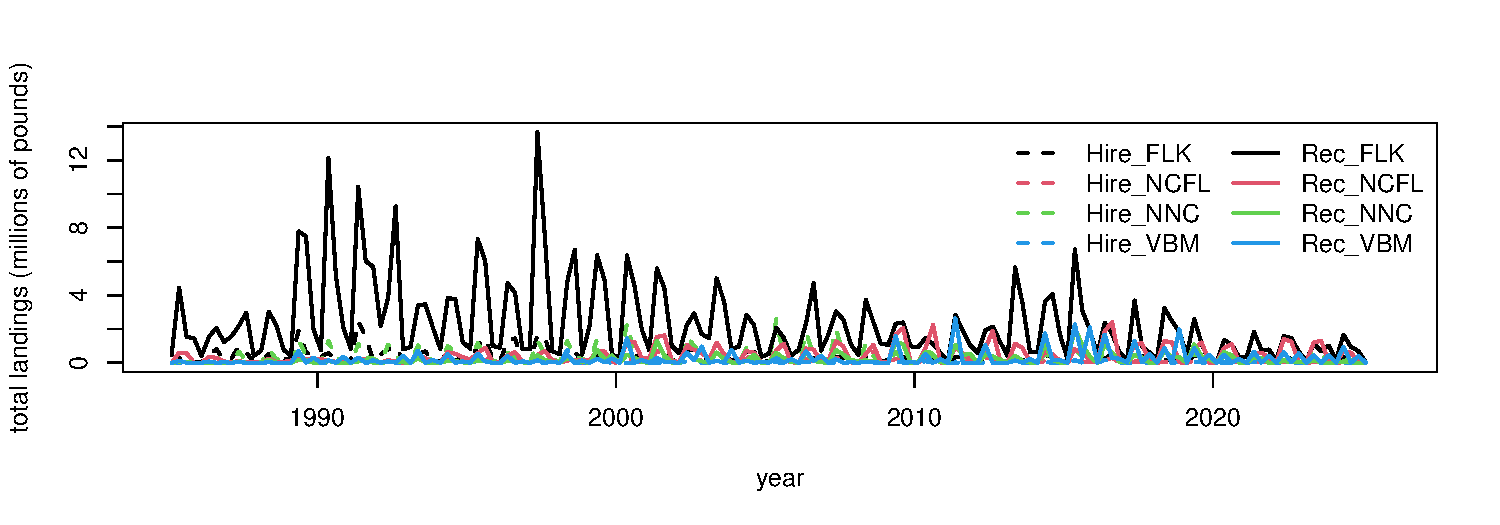
\includegraphics{MRIP_files/figure-pdf/unnamed-chunk-8-1.pdf}

\begin{Shaded}
\begin{Highlighting}[]
\CommentTok{\# check that totals match}
\FunctionTok{cbind}\NormalTok{(}\FunctionTok{colSums}\NormalTok{(findat[, }\DecValTok{3}\SpecialCharTok{:}\DecValTok{10}\NormalTok{], }\AttributeTok{na.rm =}\NormalTok{ T), }\FunctionTok{colSums}\NormalTok{(fin[}\SpecialCharTok{{-}}\FunctionTok{c}\NormalTok{(}\DecValTok{1}\SpecialCharTok{:}\DecValTok{5}\NormalTok{), ], }\AttributeTok{na.rm =}\NormalTok{ T))}
\end{Highlighting}
\end{Shaded}

\begin{verbatim}
               [,1]      [,2]
Hire_FLK   55604999  54887476
Hire_NCFL  16909916  16736926
Hire_NNC   57944903  57886388
Hire_VBM    5836953   5828072
Rec_FLK   371462933 363537632
Rec_NCFL   70803866  69641157
Rec_NNC    32556596  32479119
Rec_VBM    40081529  39968585
\end{verbatim}

\begin{Shaded}
\begin{Highlighting}[]
\CommentTok{\# the values should be close but slightly \textgreater{}1 because the last data set includes December 1985 data as part of 1986}
\FunctionTok{colSums}\NormalTok{(findat[, }\DecValTok{3}\SpecialCharTok{:}\DecValTok{10}\NormalTok{], }\AttributeTok{na.rm =}\NormalTok{ T) }\SpecialCharTok{/} \FunctionTok{colSums}\NormalTok{(fin[}\SpecialCharTok{{-}}\FunctionTok{c}\NormalTok{(}\DecValTok{1}\SpecialCharTok{:}\DecValTok{5}\NormalTok{), ], }\AttributeTok{na.rm =}\NormalTok{ T)}
\end{Highlighting}
\end{Shaded}

\begin{verbatim}
 Hire_FLK Hire_NCFL  Hire_NNC  Hire_VBM   Rec_FLK  Rec_NCFL   Rec_NNC   Rec_VBM 
 1.013073  1.010336  1.001011  1.001524  1.021800  1.016696  1.002385  1.002826 
\end{verbatim}

Here we will format the data for input to the operating model.

\begin{Shaded}
\begin{Highlighting}[]
\NormalTok{tab3 }\OtherTok{\textless{}{-}}\NormalTok{ findat}

\NormalTok{flt }\OtherTok{\textless{}{-}} \FunctionTok{c}\NormalTok{(}\FunctionTok{rep}\NormalTok{(}\StringTok{"Hire"}\NormalTok{, }\FunctionTok{nrow}\NormalTok{(tab3)}\SpecialCharTok{*}\DecValTok{4}\NormalTok{), }\FunctionTok{rep}\NormalTok{(}\StringTok{"Rec"}\NormalTok{, }\FunctionTok{nrow}\NormalTok{(tab3)}\SpecialCharTok{*}\DecValTok{4}\NormalTok{))}
  
\NormalTok{yrmon }\OtherTok{\textless{}{-}} \FunctionTok{as.numeric}\NormalTok{(tab3}\SpecialCharTok{$}\NormalTok{yrseas)}
\NormalTok{yrs }\OtherTok{\textless{}{-}} \FunctionTok{floor}\NormalTok{(yrmon)}
\NormalTok{qrt }\OtherTok{\textless{}{-}}\NormalTok{ (yrmon }\SpecialCharTok{{-}} \FunctionTok{floor}\NormalTok{(yrmon)) }\SpecialCharTok{*} \DecValTok{4} \SpecialCharTok{+} \FloatTok{0.5}
\NormalTok{area }\OtherTok{\textless{}{-}} \FunctionTok{c}\NormalTok{(}\FunctionTok{rep}\NormalTok{(}\StringTok{"FLK"}\NormalTok{, }\FunctionTok{nrow}\NormalTok{(tab3)), }\FunctionTok{rep}\NormalTok{(}\StringTok{"NCFL"}\NormalTok{, }\FunctionTok{nrow}\NormalTok{(tab3)), }
          \FunctionTok{rep}\NormalTok{(}\StringTok{"NNC"}\NormalTok{, }\FunctionTok{nrow}\NormalTok{(tab3)), }\FunctionTok{rep}\NormalTok{(}\StringTok{"VBM"}\NormalTok{, }\FunctionTok{nrow}\NormalTok{(tab3)))}
\NormalTok{area }\OtherTok{\textless{}{-}} \FunctionTok{rep}\NormalTok{(area, }\DecValTok{2}\NormalTok{)}

\NormalTok{findat1 }\OtherTok{\textless{}{-}} \FunctionTok{data.frame}\NormalTok{(yrs, qrt, flt, area, }\FunctionTok{matrix}\NormalTok{(}\FunctionTok{as.matrix}\NormalTok{(tab3[,}\DecValTok{3}\SpecialCharTok{:}\DecValTok{10}\NormalTok{])))}
\FunctionTok{names}\NormalTok{(findat1) }\OtherTok{\textless{}{-}} \FunctionTok{c}\NormalTok{(}\StringTok{"Year"}\NormalTok{, }\StringTok{"Quarter"}\NormalTok{, }\StringTok{"Fleet"}\NormalTok{, }\StringTok{"Area"}\NormalTok{, }\StringTok{"Catch\_lbs"}\NormalTok{)}
\FunctionTok{head}\NormalTok{(findat1)}
\end{Highlighting}
\end{Shaded}

\begin{verbatim}
  Year Quarter Fleet Area Catch_lbs
1 1985       1  Hire  FLK   4462.09
2 1985       2  Hire  FLK 253487.38
3 1985       3  Hire  FLK 380811.37
4 1985       4  Hire  FLK  41469.99
5 1986       1  Hire  FLK  40545.41
6 1986       2  Hire  FLK 501184.61
\end{verbatim}

\begin{Shaded}
\begin{Highlighting}[]
\CommentTok{\#plot(findat1$Catch\_lbs, type = "l")}
\CommentTok{\#plot(findat1$Catch\_lbs \textasciitilde{} factor(findat1$Area))}
\CommentTok{\#plot(findat1$Catch\_lbs \textasciitilde{} factor(findat1$Quarter))}
\CommentTok{\#plot(findat1$Catch\_lbs \textasciitilde{} factor(findat1$Year))}

\NormalTok{findat1 }\OtherTok{\textless{}{-}}\NormalTok{ findat1[}\FunctionTok{which}\NormalTok{(findat1}\SpecialCharTok{$}\NormalTok{Year }\SpecialCharTok{\textless{}=} \DecValTok{2022}\NormalTok{), ]}
\NormalTok{findat1 }\OtherTok{\textless{}{-}}\NormalTok{ findat1[}\FunctionTok{which}\NormalTok{(findat1}\SpecialCharTok{$}\NormalTok{Year }\SpecialCharTok{\textgreater{}=} \DecValTok{1986}\NormalTok{), ]}
\CommentTok{\#apply(findat1, 2, table)}

\NormalTok{findat }\OtherTok{\textless{}{-}}\NormalTok{ findat[}\FunctionTok{which}\NormalTok{(findat}\SpecialCharTok{$}\NormalTok{year }\SpecialCharTok{\textgreater{}=}\DecValTok{1986} \SpecialCharTok{\&}\NormalTok{ findat}\SpecialCharTok{$}\NormalTok{year }\SpecialCharTok{\textless{}=} \DecValTok{2022}\NormalTok{), ]}
\CommentTok{\#check that the numbers are exactly the same}
\FunctionTok{tapply}\NormalTok{(findat1}\SpecialCharTok{$}\NormalTok{Catch\_lbs, }\FunctionTok{list}\NormalTok{(findat1}\SpecialCharTok{$}\NormalTok{Area, findat1}\SpecialCharTok{$}\NormalTok{Fleet), sum, }\AttributeTok{na.rm =}\NormalTok{ T)}
\end{Highlighting}
\end{Shaded}

\begin{verbatim}
         Hire       Rec
FLK  54012811 357091651
NCFL 16532764  65643193
NNC  56097190  32197622
VBM   5736592  37749487
\end{verbatim}

\begin{Shaded}
\begin{Highlighting}[]
\FunctionTok{colSums}\NormalTok{(findat[}\DecValTok{3}\SpecialCharTok{:}\DecValTok{10}\NormalTok{], }\AttributeTok{na.rm =}\NormalTok{ T)}
\end{Highlighting}
\end{Shaded}

\begin{verbatim}
 Hire_FLK Hire_NCFL  Hire_NNC  Hire_VBM   Rec_FLK  Rec_NCFL   Rec_NNC   Rec_VBM 
 54012811  16532764  56097190   5736592 357091651  65643193  32197622  37749487 
\end{verbatim}

\begin{Shaded}
\begin{Highlighting}[]
\CommentTok{\# output final numbers in correct format}
\FunctionTok{write.csv}\NormalTok{(findat1, }\AttributeTok{file =} \StringTok{"data/FINAL\_files/rec\_catch\_TomFormat.csv"}\NormalTok{, }\AttributeTok{row.names =} \ConstantTok{FALSE}\NormalTok{)}
\end{Highlighting}
\end{Shaded}

\bookmarksetup{startatroot}

\chapter{NOAA Fisheries commercial
data}\label{noaa-fisheries-commercial-data}

We do not display the commercial data analysis here because it is based
on logbook reporting and trip ticket databases, which both contain
confidential data. The code for processing the commercial data can be
seen in the file ``commercial.R'' and the steps are outlined below.

\section{Analysis of logbook data}\label{analysis-of-logbook-data}

We first use the pelagic longline logbook data to understand how the
fleet operates in the high seas on a seasonal basis. These numbers are
used later to estimate the seasonality of the international landings,
because those are only reported on an annual basis but quarterly values
are needed.

The steps are as follows: 1. Read in the pelagic longline data which
contains set level entries including location of fishing, target
species, gear used, other details of the fishing trip and number of
dolphin caught, discarded alive, discarded dead, and the total pounds of
dolphin kept. 2. Format the longitude and latitude of the sets into
decimal degrees, and find the points that fall within each of the seven
polygons representing the areas of the operating model. Check that
subsetting was done correctly and add and area identifier. 3. Look at
the characteristics of the dolphin catch and calculate the discard rates
by trip. Dead discarding rate is found to be 1.4\% on average and total
discard rate is 2.9\% on average. 4. Standardize date formatting and add
identifier for season (quarter). Specify a new year variable to allow
December to be grouped with January and February. 5. Summarize the total
dolphin catch (in pounds) by year, quarter, and area. 6. Convert the
total pounds by year-quarter and area to proportions such that each
year-quarter combination has four seasonal proportions summing to 1.
Save the matrix of proportions for later analysis.

\begin{figure}[H]

{\centering 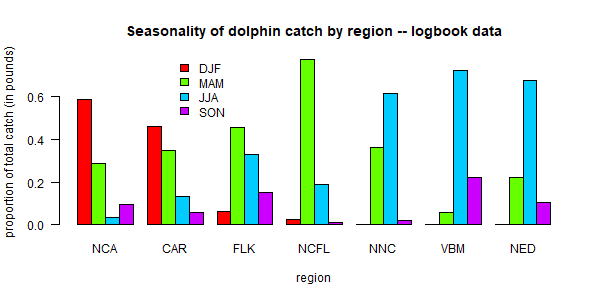
\includegraphics{plots/PLL_seasonality.png}

}

\caption{Seasonality of the pelagic longline fleet according to the
logbook data. Figure shows the proportion of dolphin catch occurring in
each season, for each region of the operating model.}

\end{figure}%

\section{Analysis of trip ticket
data}\label{analysis-of-trip-ticket-data}

Not all of the commercial dolphin catch activity is reported in the
logbooks because dolphin are targeted via a variety of permits and gear
types, not all of which have the same reporting requirements. Therefore,
in order to parse the commercial catches by year, area and quarter, we
use the commercial trip ticket data compiled by NOAA Fisheries. These
are the same data used for quota monitoring and thus are the best
representation of the total catch.

The steps are as follows: 1. Read in the trip ticket data file, which
contains commercial dolphinfish landings for the Atlantic coast from
1986-2023, including all landings by year even if the gear type or area
is unknown. The dataset specifies the year and month of landing, an area
of fishing, gear, and the state where landed. Pounds are in units of
whole weight. 2. Read in operating model regions and classify the list
of logbook areas into those seven regions. Assign each reported area to
an operating model region accordingly. 3. Standardize date formatting
and add identifier for season (quarter). Specify a new year variable to
allow December to be grouped with January and February. 4. Summarize the
landings by year-quarter, gear (PLL gear vs.~other gears) and region. 5.
For most combinations of year-quarter, region and gear, there are
substantial landings for which the area of fishing is unknown and
therefore the region cannot be defined. We assume that those landings
follow the same distribution with regard to region as the other landings
for that year-quarter and gear combination. For each year-quarter/gear
combination, we calculate the proportion of catch that occurs in each of
the seven regions. The total landings of unknown regions are multiplied
by those proportions and then added to the landings from known regions.
In cases where none of the areas are known for that year-quarter/gear
combination, proportions from the quarter immediately previous to that
quarter are used. Sum the landings by gear type to get the total
landings for each year-quarter and region. 6. Reformat the data
according to the specifications needed for input to the operating model
(columns specifying the year, quarter, fleet, area and total catch). 7.
Sum landings by year from the original data file and the final outputs
to ensure that data were processed correctly and no catch is missing.

\begin{figure}[H]

{\centering 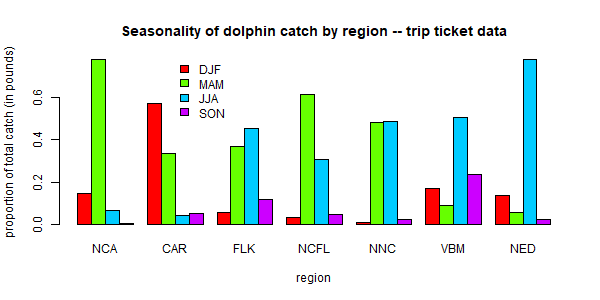
\includegraphics{plots/tripticket_seasonality.png}

}

\caption{Seasonality of the commercial dolphin catch according to the
trip ticket data. Figure shows the proportion of dolphin catch occurring
in each season, for each region of the operating model.}

\end{figure}%

\bookmarksetup{startatroot}

\chapter{Analysis of international landings in the high
seas}\label{analysis-of-international-landings-in-the-high-seas}

Here we will explore commercial and recreational landings data as
estimated by the \href{https://www.seaaroundus.org/data/\#/eez}{Sea
Around Us Project}. This data set includes reported data for fisheries
worldwide as well as reconstructed estimates for unreported landings.
For each country, project scientists assemble available data on landings
and use additional sociological and fishing data plus expert information
and opinion, to produce their best estimates of total landings from all
fishing sectors and for all species globally.

\section{Data access and upload}\label{data-access-and-upload-1}

The high seas data are accessed in the Basic Search
\href{https://www.seaaroundus.org/data/\#/highseas}{High seas section of
the site}. The individual regions can be clicked on (e.g., Atlantic,
Western Central) and then the data are downloaded using the Download
Data button.

The current version of data in use is version 50.1, accessed June 2024
(the data files can be found on github in the
SEFSC-dolphin-analyses/data /SAU/ folder). This was still the most
recent version of data available as of September 2025.

\section{Read in the high seas
landings}\label{read-in-the-high-seas-landings}

First we read in the high seas landings for the Western Central Atlantic
and Northwest Atlantic zones. These are equivalent to FAO areas 21 and
31.

\begin{Shaded}
\begin{Highlighting}[]
\CommentTok{\# clear workspace}
\FunctionTok{rm}\NormalTok{(}\AttributeTok{list =} \FunctionTok{ls}\NormalTok{())}

\ControlFlowTok{if}\NormalTok{(}\SpecialCharTok{!}\FunctionTok{require}\NormalTok{(}\StringTok{"pals"}\NormalTok{)) }\FunctionTok{install.packages}\NormalTok{(}\StringTok{"pals"}\NormalTok{)}
\FunctionTok{library}\NormalTok{(pals)}

\CommentTok{\# find data files}
\NormalTok{hslis }\OtherTok{\textless{}{-}} \FunctionTok{dir}\NormalTok{(}\StringTok{"data/SAU/"}\NormalTok{)[}\FunctionTok{grep}\NormalTok{(}\StringTok{"HighSeas"}\NormalTok{, }\FunctionTok{dir}\NormalTok{(}\StringTok{"data/SAU/"}\NormalTok{))]}

\CommentTok{\# identify areas 21 and 31}
\NormalTok{hslis[}\DecValTok{1}\NormalTok{]; hslis[}\DecValTok{3}\NormalTok{]   }
\end{Highlighting}
\end{Shaded}

\begin{verbatim}
[1] "SAU HighSeas 21 v50-1.csv"
\end{verbatim}

\begin{verbatim}
[1] "SAU HighSeas 31 v50-1.csv"
\end{verbatim}

\begin{Shaded}
\begin{Highlighting}[]
\CommentTok{\#download data}
\NormalTok{h1 }\OtherTok{\textless{}{-}} \FunctionTok{read.csv}\NormalTok{(}\FunctionTok{paste0}\NormalTok{(}\StringTok{"data/SAU/"}\NormalTok{, hslis[}\DecValTok{1}\NormalTok{]))   }
\NormalTok{h3 }\OtherTok{\textless{}{-}} \FunctionTok{read.csv}\NormalTok{(}\FunctionTok{paste0}\NormalTok{(}\StringTok{"data/SAU/"}\NormalTok{, hslis[}\DecValTok{3}\NormalTok{]))}

\CommentTok{\# confirm correct areas}
\CommentTok{\#unique(h1$area\_name)}
\CommentTok{\#unique(h3$area\_name)}

\NormalTok{hs }\OtherTok{\textless{}{-}} \FunctionTok{rbind}\NormalTok{(h1, h3) }
\end{Highlighting}
\end{Shaded}

We extract the data for dolphinfish and look at the characteristics of
the landings. Most of the landings are in the Western Central Atlantic,
and the primary fishing entities are Venezuela and Saint Lucia. The
fishing sector is all industrial, and the vast majority of the catch is
reported landings, with only a tiny fraction of discards or unreported
landings listed in the database. The gear type is primarily long line.

\begin{Shaded}
\begin{Highlighting}[]
\CommentTok{\# check species name and filter out dolphinfish}
\FunctionTok{unique}\NormalTok{(hs}\SpecialCharTok{$}\NormalTok{common\_name)[}\FunctionTok{grep}\NormalTok{(}\StringTok{"dolphin"}\NormalTok{, }\FunctionTok{unique}\NormalTok{(hs}\SpecialCharTok{$}\NormalTok{common\_name))]}
\end{Highlighting}
\end{Shaded}

\begin{verbatim}
[1] "Common dolphinfish"
\end{verbatim}

\begin{Shaded}
\begin{Highlighting}[]
\NormalTok{hs }\OtherTok{\textless{}{-}}\NormalTok{ hs[}\FunctionTok{which}\NormalTok{(hs}\SpecialCharTok{$}\NormalTok{common\_name }\SpecialCharTok{==} \StringTok{"Common dolphinfish"}\NormalTok{), ]}

\CommentTok{\# look at the categories within each column of data}
\FunctionTok{apply}\NormalTok{(hs[}\DecValTok{1}\SpecialCharTok{:}\DecValTok{13}\NormalTok{], }\DecValTok{2}\NormalTok{, table)}
\end{Highlighting}
\end{Shaded}

\begin{verbatim}
$area_name

      Atlantic, Northwest Atlantic, Western Central 
                      113                       160 

$area_type

high_seas 
      273 

$year

1985 1986 1999 2000 2001 2002 2003 2004 2005 2006 2007 2008 2009 2010 2011 2012 
   1    1    1    1    1    1    1    6    4    1    5   10    5    8   10   12 
2013 2014 2015 2016 2017 2018 2019 
  24   22   30   33   33   29   34 

$scientific_name

Coryphaena hippurus 
                273 

$common_name

Common dolphinfish 
               273 

$functional_group

Large pelagics (>=90 cm) 
                     273 

$commercial_group

Perch-likes 
        273 

$fishing_entity

                      Barbados                         Belize 
                             6                              3 
                        Brazil                         Canada 
                            19                             18 
                        Guyana                         Panama 
                             1                              1 
                   Saint Lucia Saint Vincent & the Grenadines 
                             5                             28 
                         Spain                       Suriname 
                            80                              1 
             Trinidad & Tobago                            USA 
                            14                             74 
                     Venezuela 
                            23 

$fishing_sector

Industrial 
       273 

$catch_type

Discards Landings 
       5      268 

$reporting_status

  Reported Unreported 
       253         20 

$gear_type

artisanal fishing gear           bottom trawl                gillnet 
                     7                      9                     11 
            hand lines               longline             mixed gear 
                    17                    187                      1 
         pole and line          pots or traps      unknown by source 
                    19                      9                     13 

$end_use_type

                         Direct human consumption    Fishmeal and fish oil 
                       5                      194                       37 
                   Other 
                      37 
\end{verbatim}

\begin{Shaded}
\begin{Highlighting}[]
\CommentTok{\# convert from metric tonnes to pounds}
\NormalTok{hs}\SpecialCharTok{$}\NormalTok{pounds }\OtherTok{\textless{}{-}}\NormalTok{ hs}\SpecialCharTok{$}\NormalTok{tonnes }\SpecialCharTok{*} \DecValTok{1000} \SpecialCharTok{*} \FloatTok{2.20462}

\CommentTok{\# produce barplot of key data fields}
\FunctionTok{par}\NormalTok{(}\AttributeTok{mar =} \FunctionTok{c}\NormalTok{(}\DecValTok{3}\NormalTok{, }\DecValTok{20}\NormalTok{, }\DecValTok{3}\NormalTok{, }\DecValTok{1}\NormalTok{), }\AttributeTok{mfrow =} \FunctionTok{c}\NormalTok{(}\DecValTok{3}\NormalTok{, }\DecValTok{2}\NormalTok{), }\AttributeTok{mex =} \FloatTok{0.5}\NormalTok{)}
\FunctionTok{barplot}\NormalTok{(}\FunctionTok{tapply}\NormalTok{(hs}\SpecialCharTok{$}\NormalTok{pounds}\SpecialCharTok{/}\DecValTok{10}\SpecialCharTok{\^{}}\DecValTok{6}\NormalTok{, hs}\SpecialCharTok{$}\NormalTok{area\_name, sum, }\AttributeTok{na.rm =}\NormalTok{ T), }\AttributeTok{las =} \DecValTok{2}\NormalTok{, }\AttributeTok{xlab =} \StringTok{"millions of pounds"}\NormalTok{, }\AttributeTok{main =} \StringTok{"Area name"}\NormalTok{, }\AttributeTok{horiz =}\NormalTok{ T)}
\CommentTok{\#barplot(tapply(hs$pounds/10\^{}6, hs$area\_type, sum, na.rm = T), las = 2, ylab = "millions of pounds", main = "Area type")}
\CommentTok{\#barplot(tapply(hs$pounds/10\^{}6, hs$year, sum, na.rm = T), las = 2, ylab = "millions of pounds", main = "Year")}
\FunctionTok{barplot}\NormalTok{(}\FunctionTok{tapply}\NormalTok{(hs}\SpecialCharTok{$}\NormalTok{pounds}\SpecialCharTok{/}\DecValTok{10}\SpecialCharTok{\^{}}\DecValTok{6}\NormalTok{, hs}\SpecialCharTok{$}\NormalTok{fishing\_entity, sum, }\AttributeTok{na.rm =}\NormalTok{ T), }\AttributeTok{las =} \DecValTok{2}\NormalTok{, }\AttributeTok{xlab =} \StringTok{"millions of pounds"}\NormalTok{, }\AttributeTok{main =} \StringTok{"Fishing entity"}\NormalTok{, }\AttributeTok{horiz =}\NormalTok{ T)}
\FunctionTok{barplot}\NormalTok{(}\FunctionTok{tapply}\NormalTok{(hs}\SpecialCharTok{$}\NormalTok{pounds}\SpecialCharTok{/}\DecValTok{10}\SpecialCharTok{\^{}}\DecValTok{6}\NormalTok{, hs}\SpecialCharTok{$}\NormalTok{fishing\_sector, sum, }\AttributeTok{na.rm =}\NormalTok{ T), }\AttributeTok{las =} \DecValTok{2}\NormalTok{, }\AttributeTok{xlab =} \StringTok{"millions of pounds"}\NormalTok{, }\AttributeTok{main =} \StringTok{"Fishing sector"}\NormalTok{, }\AttributeTok{horiz =}\NormalTok{ T)}
\FunctionTok{barplot}\NormalTok{(}\FunctionTok{tapply}\NormalTok{(hs}\SpecialCharTok{$}\NormalTok{pounds}\SpecialCharTok{/}\DecValTok{10}\SpecialCharTok{\^{}}\DecValTok{6}\NormalTok{, hs}\SpecialCharTok{$}\NormalTok{catch\_type, sum, }\AttributeTok{na.rm =}\NormalTok{ T), }\AttributeTok{las =} \DecValTok{2}\NormalTok{, }\AttributeTok{xlab =} \StringTok{"millions of pounds"}\NormalTok{, }\AttributeTok{main =} \StringTok{"Catch type"}\NormalTok{, }\AttributeTok{horiz =}\NormalTok{ T)}
\FunctionTok{barplot}\NormalTok{(}\FunctionTok{tapply}\NormalTok{(hs}\SpecialCharTok{$}\NormalTok{pounds}\SpecialCharTok{/}\DecValTok{10}\SpecialCharTok{\^{}}\DecValTok{6}\NormalTok{, hs}\SpecialCharTok{$}\NormalTok{reporting\_status, sum, }\AttributeTok{na.rm =}\NormalTok{ T), }\AttributeTok{las =} \DecValTok{2}\NormalTok{, }\AttributeTok{xlab =} \StringTok{"millions of pounds"}\NormalTok{, }\AttributeTok{main =} \StringTok{"Reporting status"}\NormalTok{, }\AttributeTok{horiz =}\NormalTok{ T)}
\FunctionTok{barplot}\NormalTok{(}\FunctionTok{tapply}\NormalTok{(hs}\SpecialCharTok{$}\NormalTok{pounds}\SpecialCharTok{/}\DecValTok{10}\SpecialCharTok{\^{}}\DecValTok{6}\NormalTok{, hs}\SpecialCharTok{$}\NormalTok{gear\_type, sum, }\AttributeTok{na.rm =}\NormalTok{ T), }\AttributeTok{las =} \DecValTok{2}\NormalTok{, }\AttributeTok{xlab =} \StringTok{"millions of pounds"}\NormalTok{, }\AttributeTok{main =} \StringTok{"Gear type"}\NormalTok{, }\AttributeTok{horiz =}\NormalTok{ T)}
\end{Highlighting}
\end{Shaded}

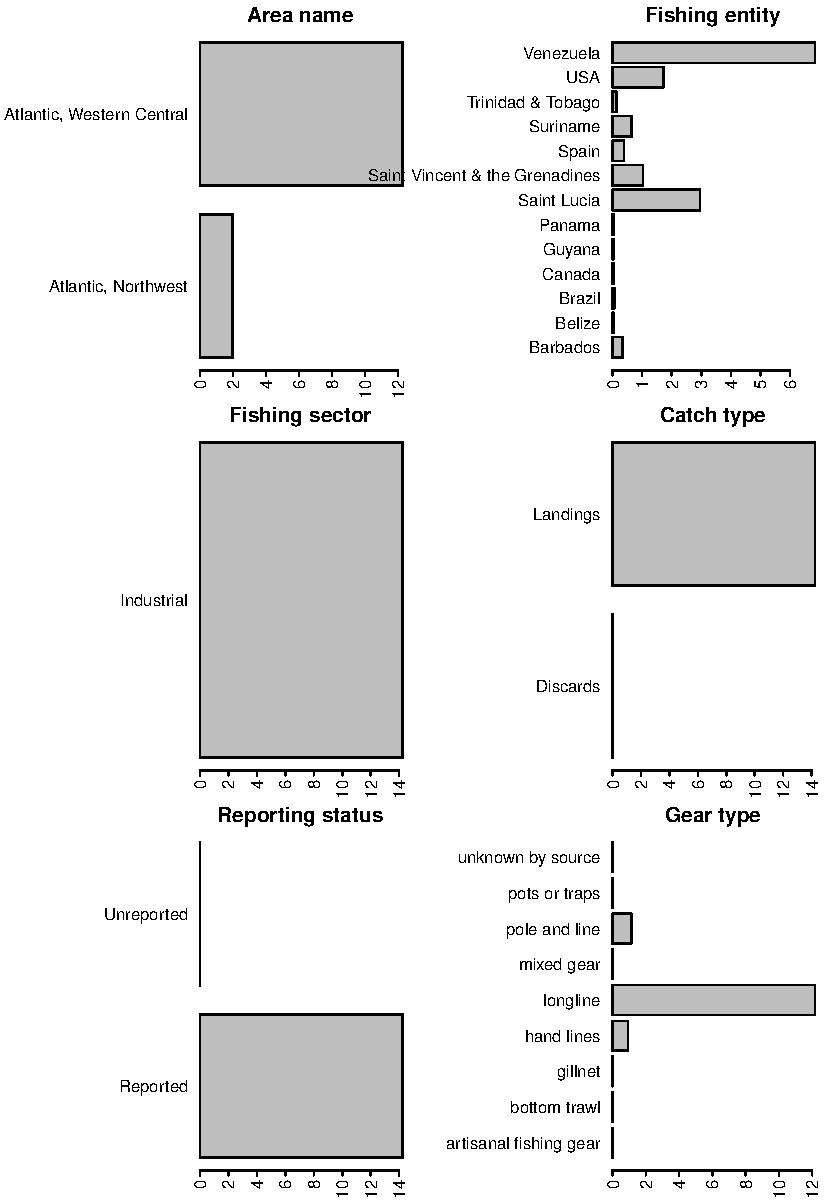
\includegraphics{SAU_highseas_files/figure-pdf/unnamed-chunk-2-1.pdf}

\begin{Shaded}
\begin{Highlighting}[]
\FunctionTok{round}\NormalTok{(}\FunctionTok{tapply}\NormalTok{(hs}\SpecialCharTok{$}\NormalTok{pounds, hs}\SpecialCharTok{$}\NormalTok{catch\_type, sum, }\AttributeTok{na.rm =}\NormalTok{ T) }\SpecialCharTok{/} \FunctionTok{sum}\NormalTok{(hs}\SpecialCharTok{$}\NormalTok{pounds) }\SpecialCharTok{*} \DecValTok{100}\NormalTok{, }\DecValTok{2}\NormalTok{)   }\CommentTok{\# \textless{}\textless{} 1\% are discards}
\end{Highlighting}
\end{Shaded}

\begin{verbatim}
Discards Landings 
    0.03    99.97 
\end{verbatim}

\begin{Shaded}
\begin{Highlighting}[]
\FunctionTok{round}\NormalTok{(}\FunctionTok{tapply}\NormalTok{(hs}\SpecialCharTok{$}\NormalTok{pounds, hs}\SpecialCharTok{$}\NormalTok{reporting\_status, sum, }\AttributeTok{na.rm =}\NormalTok{ T) }\SpecialCharTok{/} \FunctionTok{sum}\NormalTok{(hs}\SpecialCharTok{$}\NormalTok{pounds) }\SpecialCharTok{*} \DecValTok{100}\NormalTok{, }\DecValTok{2}\NormalTok{)  }\CommentTok{\# \textless{}\textless{} 1\% are unreported}
\end{Highlighting}
\end{Shaded}

\begin{verbatim}
  Reported Unreported 
     99.97       0.03 
\end{verbatim}

\section{Summarize the high seas
landings}\label{summarize-the-high-seas-landings}

We plot the annual catches by fishing entity to look at trends over
time.

\begin{Shaded}
\begin{Highlighting}[]
\NormalTok{hs}\SpecialCharTok{$}\NormalTok{fishing\_entity }\OtherTok{\textless{}{-}} \FunctionTok{as.factor}\NormalTok{(hs}\SpecialCharTok{$}\NormalTok{fishing\_entity)}
\NormalTok{hs}\SpecialCharTok{$}\NormalTok{fishing\_entity }\OtherTok{\textless{}{-}} \FunctionTok{droplevels}\NormalTok{(hs}\SpecialCharTok{$}\NormalTok{fishing\_entity)}

\FunctionTok{par}\NormalTok{(}\AttributeTok{mar =} \FunctionTok{c}\NormalTok{(}\DecValTok{5}\NormalTok{, }\DecValTok{5}\NormalTok{, }\DecValTok{3}\NormalTok{, }\DecValTok{1}\NormalTok{), }\AttributeTok{mfrow =} \FunctionTok{c}\NormalTok{(}\DecValTok{1}\NormalTok{, }\DecValTok{1}\NormalTok{))}
\NormalTok{tab }\OtherTok{\textless{}{-}} \FunctionTok{tapply}\NormalTok{(hs}\SpecialCharTok{$}\NormalTok{pounds, }\FunctionTok{list}\NormalTok{(hs}\SpecialCharTok{$}\NormalTok{year, hs}\SpecialCharTok{$}\NormalTok{fishing\_entity), sum, }\AttributeTok{na.rm =}\NormalTok{ T)}
\FunctionTok{matplot}\NormalTok{(}\FunctionTok{as.numeric}\NormalTok{(}\FunctionTok{rownames}\NormalTok{(tab)), tab}\SpecialCharTok{/}\DecValTok{10}\SpecialCharTok{\^{}}\DecValTok{6}\NormalTok{, }\AttributeTok{type =} \StringTok{"l"}\NormalTok{, }\AttributeTok{col =} \FunctionTok{glasbey}\NormalTok{(}\FunctionTok{ncol}\NormalTok{(tab)), }\AttributeTok{lty =} \DecValTok{1}\NormalTok{, }\AttributeTok{lwd =} \DecValTok{2}\NormalTok{, }\AttributeTok{xlab =} \StringTok{"year"}\NormalTok{, }\AttributeTok{ylab =} \StringTok{"total catch (millions of pounds)"}\NormalTok{, }
        \AttributeTok{main =} \StringTok{"High seas Western Central Atlantic dolphin catch"}\NormalTok{)}
\FunctionTok{legend}\NormalTok{(}\StringTok{"topleft"}\NormalTok{, }\FunctionTok{colnames}\NormalTok{(tab), }\AttributeTok{col =} \FunctionTok{glasbey}\NormalTok{(}\FunctionTok{ncol}\NormalTok{(tab)), }\AttributeTok{lty =} \DecValTok{1}\NormalTok{, }\AttributeTok{lwd =} \DecValTok{2}\NormalTok{, }\AttributeTok{cex =} \FloatTok{0.8}\NormalTok{, }\AttributeTok{bty =} \StringTok{"n"}\NormalTok{)}
\end{Highlighting}
\end{Shaded}

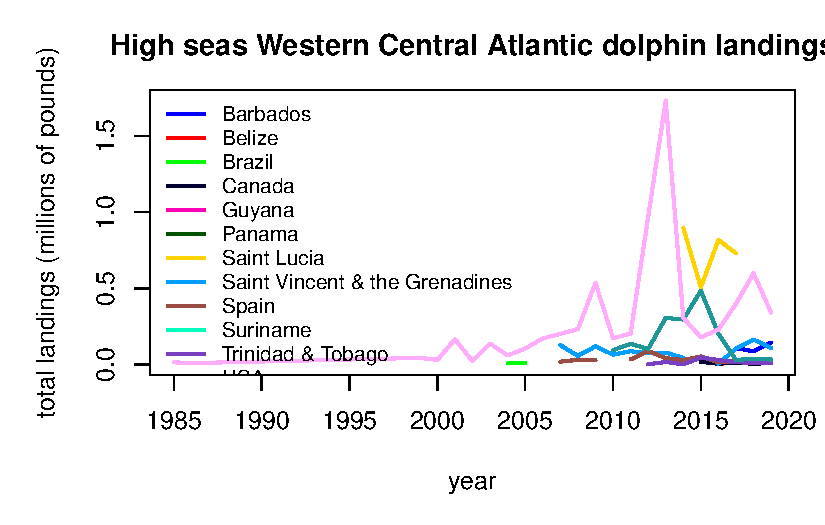
\includegraphics{SAU_highseas_files/figure-pdf/unnamed-chunk-3-1.pdf}

Finally we output the subset of high seas dolphin catch for the two
areas. Because we have already accounted for the USA landings in our
national reporting and are aiming to only summarize international
landings here, we filter out the USA landings from the Sea Around Us
database.

\begin{Shaded}
\begin{Highlighting}[]
\NormalTok{hs }\OtherTok{\textless{}{-}}\NormalTok{ hs[}\FunctionTok{which}\NormalTok{(hs}\SpecialCharTok{$}\NormalTok{fishing\_entity }\SpecialCharTok{!=} \StringTok{"USA"}\NormalTok{), ]}

\NormalTok{hs}\SpecialCharTok{$}\NormalTok{year }\OtherTok{\textless{}{-}} \FunctionTok{factor}\NormalTok{(hs}\SpecialCharTok{$}\NormalTok{year, }\AttributeTok{levels =} \DecValTok{1950}\SpecialCharTok{:}\DecValTok{2019}\NormalTok{)}
\NormalTok{tab }\OtherTok{\textless{}{-}} \FunctionTok{tapply}\NormalTok{(hs}\SpecialCharTok{$}\NormalTok{pounds, }\FunctionTok{list}\NormalTok{(hs}\SpecialCharTok{$}\NormalTok{year, hs}\SpecialCharTok{$}\NormalTok{area\_name), sum, }\AttributeTok{na.rm =}\NormalTok{ T)}
\NormalTok{tab[}\FunctionTok{is.na}\NormalTok{(tab)] }\OtherTok{\textless{}{-}} \DecValTok{0}
\FunctionTok{tail}\NormalTok{(tab, }\DecValTok{40}\NormalTok{)}
\end{Highlighting}
\end{Shaded}

\begin{verbatim}
     Atlantic, Northwest Atlantic, Western Central
1980               0.000                     0.000
1981               0.000                     0.000
1982               0.000                     0.000
1983               0.000                     0.000
1984               0.000                     0.000
1985               0.000                 14037.129
1986               0.000                  8748.399
1987               0.000                     0.000
1988               0.000                     0.000
1989               0.000                     0.000
1990               0.000                     0.000
1991               0.000                     0.000
1992               0.000                     0.000
1993               0.000                     0.000
1994               0.000                     0.000
1995               0.000                     0.000
1996               0.000                     0.000
1997               0.000                     0.000
1998               0.000                     0.000
1999               0.000                 43168.296
2000               0.000                 30284.627
2001               0.000                164272.223
2002               0.000                 22147.477
2003               0.000                137103.181
2004               0.000                 66058.258
2005               0.000                115171.863
2006               0.000                170522.101
2007           14687.527                330838.620
2008           28552.636                340863.719
2009           18719.121                662720.661
2010            4510.085                232093.837
2011           21589.424                300498.224
2012           72398.812               1059210.392
2013           34741.604               2471791.396
2014           27922.953               1247462.983
2015           90313.638                710059.125
2016           15319.433               1094893.891
2017           34806.933               1374259.739
2018           29328.358                885814.754
2019           21870.621                632747.157
\end{verbatim}

\begin{Shaded}
\begin{Highlighting}[]
\CommentTok{\# write summary to merge with EEZ data }
\FunctionTok{write.csv}\NormalTok{(tab, }\AttributeTok{file =} \StringTok{"data/SAU/high\_seas\_by\_year.csv"}\NormalTok{)}
\end{Highlighting}
\end{Shaded}

\section{Distribute the high seas landings across quarters of the
year}\label{distribute-the-high-seas-landings-across-quarters-of-the-year}

The international landings are only reported as annual catches and do
not have any month or season associated with them. However, the MSE
operating model requires seasonal catches. The majority of the
international landings are caught by longline, so we will assume that
the fleet distribution of the U.S. pelagic longline is representative of
the seasonality of the international high seas fleets. Now we parse the
annual catches according to the seasonality of the U.S. fleet.

At the time of analysis, the SAU database only contained catches to
2019, so we interpolated the 2019 values to cover years 2020 - 2022.

\begin{Shaded}
\begin{Highlighting}[]
\CommentTok{\# read in the percentage of the catch by area and year{-}quarter combinations from the U.S. PLL}
\FunctionTok{load}\NormalTok{(}\StringTok{"data/outputs/per\_PLLcatch\_by\_area\_yearquarter.RData"}\NormalTok{)  }

\NormalTok{tab }\OtherTok{\textless{}{-}}\NormalTok{ tab[}\FunctionTok{which}\NormalTok{(}\FunctionTok{rownames}\NormalTok{(tab) }\SpecialCharTok{\textgreater{}=} \DecValTok{1997}\NormalTok{), ]  }\CommentTok{\# PLL data are only available from 1997 on }
\CommentTok{\#tab[nrow(tab), ]}
\NormalTok{tab }\OtherTok{\textless{}{-}} \FunctionTok{rbind}\NormalTok{(tab, tab[}\FunctionTok{nrow}\NormalTok{(tab), ], tab[}\FunctionTok{nrow}\NormalTok{(tab), ], tab[}\FunctionTok{nrow}\NormalTok{(tab), ])  }\CommentTok{\# interpolate 2019 catches for 2020{-}2022}
\FunctionTok{tail}\NormalTok{(tab)}
\end{Highlighting}
\end{Shaded}

\begin{verbatim}
     Atlantic, Northwest Atlantic, Western Central
2017            34806.93                 1374259.7
2018            29328.36                  885814.8
2019            21870.62                  632747.2
                21870.62                  632747.2
                21870.62                  632747.2
                21870.62                  632747.2
\end{verbatim}

\begin{Shaded}
\begin{Highlighting}[]
\NormalTok{NED }\OtherTok{\textless{}{-}}\NormalTok{ percatch[, , }\DecValTok{1}\NormalTok{]   }\CommentTok{\# create matrices for final catch data}
\NormalTok{NCA }\OtherTok{\textless{}{-}}\NormalTok{ percatch[, , }\DecValTok{1}\NormalTok{]}

\ControlFlowTok{for}\NormalTok{ (i }\ControlFlowTok{in} \DecValTok{1}\SpecialCharTok{:}\FunctionTok{ncol}\NormalTok{(percatch))  \{ }
\NormalTok{  NED[, i] }\OtherTok{\textless{}{-}}\NormalTok{ percatch[, i, }\DecValTok{7}\NormalTok{] }\SpecialCharTok{*}\NormalTok{ tab[i, }\DecValTok{1}\NormalTok{]   }\CommentTok{\# these are the percentages for the NED (Atlantic Northwest)}
\NormalTok{  NCA[, i] }\OtherTok{\textless{}{-}}\NormalTok{ percatch[, i, }\DecValTok{1}\NormalTok{] }\SpecialCharTok{*}\NormalTok{ tab[i, }\DecValTok{2}\NormalTok{]   }\CommentTok{\# these are the percentages for the NCA (Western Central Atlantic)}
\NormalTok{  \}}

\CommentTok{\# plot the parsed out data by year{-}quarter}
\NormalTok{yrs }\OtherTok{\textless{}{-}} \FunctionTok{sort}\NormalTok{(}\FunctionTok{rep}\NormalTok{(}\FunctionTok{as.numeric}\NormalTok{(}\FunctionTok{colnames}\NormalTok{(NCA)), }\DecValTok{4}\NormalTok{))}
\NormalTok{qrt }\OtherTok{\textless{}{-}} \FunctionTok{rep}\NormalTok{(}\DecValTok{1}\SpecialCharTok{:}\DecValTok{4}\NormalTok{, }\FunctionTok{length}\NormalTok{(yrs)}\SpecialCharTok{/}\DecValTok{4}\NormalTok{)}

\FunctionTok{matplot}\NormalTok{(yrs }\SpecialCharTok{+}\NormalTok{ qrt}\SpecialCharTok{/}\DecValTok{4}\NormalTok{, }\FunctionTok{cbind}\NormalTok{(}\FunctionTok{matrix}\NormalTok{(NED), }\FunctionTok{matrix}\NormalTok{(NCA))}\SpecialCharTok{/}\DecValTok{10}\SpecialCharTok{\^{}}\DecValTok{6}\NormalTok{, }\AttributeTok{lty =} \DecValTok{1}\NormalTok{, }\AttributeTok{lwd =} \DecValTok{2}\NormalTok{, }
        \AttributeTok{col =} \DecValTok{2}\SpecialCharTok{:}\DecValTok{3}\NormalTok{, }\AttributeTok{type =} \StringTok{"l"}\NormalTok{, }\AttributeTok{main =} \StringTok{"International high seas catches by quarter"}\NormalTok{, }
        \AttributeTok{xlab =} \StringTok{""}\NormalTok{, }\AttributeTok{ylab =} \StringTok{"total catch (millions of pounds)"}\NormalTok{)}
\FunctionTok{legend}\NormalTok{(}\StringTok{"topleft"}\NormalTok{, }\FunctionTok{c}\NormalTok{(}\StringTok{"NED"}\NormalTok{, }\StringTok{"NCA"}\NormalTok{), }\AttributeTok{lwd =} \DecValTok{2}\NormalTok{, }\AttributeTok{col =} \DecValTok{2}\SpecialCharTok{:}\DecValTok{3}\NormalTok{, }\AttributeTok{bty =} \StringTok{"n"}\NormalTok{)}
\end{Highlighting}
\end{Shaded}

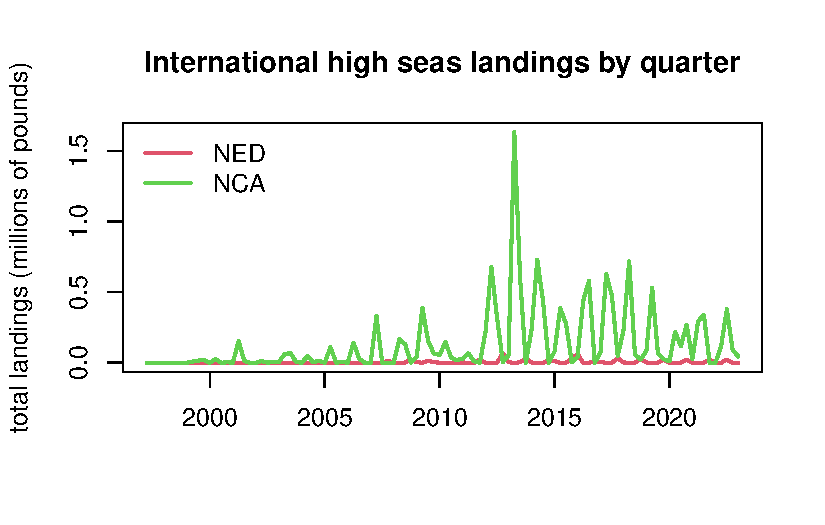
\includegraphics{SAU_highseas_files/figure-pdf/unnamed-chunk-5-1.pdf}

\begin{Shaded}
\begin{Highlighting}[]
\CommentTok{\# save NED data in this format because it needs to be combined with Canadian EEZ catches}
\FunctionTok{save}\NormalTok{(NED, }\AttributeTok{file =} \StringTok{"data/outputs/NED\_year\_quarter.RData"}\NormalTok{)}
\end{Highlighting}
\end{Shaded}

Finally, we format the data in the format for input into the operating
model. We only include NCA here, as the NED high seas catches must be
combined with international catches in territorial waters of Canada and
France in the NED region.

\begin{Shaded}
\begin{Highlighting}[]
\CommentTok{\# format for operating model}
\NormalTok{flt }\OtherTok{\textless{}{-}} \FunctionTok{rep}\NormalTok{(}\StringTok{"Intl"}\NormalTok{, }\FunctionTok{length}\NormalTok{(yrs))}
\NormalTok{are }\OtherTok{\textless{}{-}} \FunctionTok{rep}\NormalTok{(}\StringTok{"NCA"}\NormalTok{, }\FunctionTok{length}\NormalTok{(yrs))}
\NormalTok{findat }\OtherTok{\textless{}{-}} \FunctionTok{data.frame}\NormalTok{(}\FunctionTok{cbind}\NormalTok{(yrs, qrt, flt, are, }\FunctionTok{matrix}\NormalTok{(NCA)))}
\FunctionTok{names}\NormalTok{(findat) }\OtherTok{\textless{}{-}} \FunctionTok{c}\NormalTok{(}\StringTok{"Year"}\NormalTok{, }\StringTok{"Quarter"}\NormalTok{, }\StringTok{"Fleet"}\NormalTok{, }\StringTok{"Area"}\NormalTok{, }\StringTok{"Catch\_lbs"}\NormalTok{)}
\NormalTok{findat}\SpecialCharTok{$}\NormalTok{Catch\_lbs }\OtherTok{\textless{}{-}} \FunctionTok{as.numeric}\NormalTok{(findat}\SpecialCharTok{$}\NormalTok{Catch\_lbs)}
\FunctionTok{head}\NormalTok{(findat)}
\end{Highlighting}
\end{Shaded}

\begin{verbatim}
  Year Quarter Fleet Area Catch_lbs
1 1997       1  Intl  NCA         0
2 1997       2  Intl  NCA         0
3 1997       3  Intl  NCA         0
4 1997       4  Intl  NCA         0
5 1998       1  Intl  NCA         0
6 1998       2  Intl  NCA         0
\end{verbatim}

\begin{Shaded}
\begin{Highlighting}[]
\CommentTok{\#plot(findat$Catch\_lbs, type = "l")}
\CommentTok{\#plot(findat$Catch\_lbs \textasciitilde{} factor(findat$Area))}
\CommentTok{\#plot(findat$Catch\_lbs \textasciitilde{} factor(findat$Quarter))}
\CommentTok{\#plot(findat$Catch\_lbs \textasciitilde{} factor(findat$Year))}
\CommentTok{\#apply(findat, 2, table)}
\CommentTok{\#barplot(tapply(findat$Catch\_lbs, list(findat$Quarter, findat$Area), sum, na.rm = T), beside = T, col = rainbow(4))}

\FunctionTok{write.csv}\NormalTok{(findat, }\AttributeTok{file =} \StringTok{"data/FINAL\_files/NCA\_Intl\_TomFormat.csv"}\NormalTok{, }\AttributeTok{row.names =} \ConstantTok{FALSE}\NormalTok{)}
\end{Highlighting}
\end{Shaded}

\bookmarksetup{startatroot}

\chapter{Analysis of international landings in territorial
waters}\label{analysis-of-international-landings-in-territorial-waters}

\section{Data access and upload}\label{data-access-and-upload-2}

For catches within each country's exclusive economic zones, data are
downloaded from the
\href{https://www.seaaroundus.org/data/\#/topic/biodiversity}{Sea Around
Us site} (Pauly, Zeller, and Palomares, 2020.). In the Biodiversity by
Taxon Tools and Data, we filter by EEZ for All regions, and then filter
by Taxon at the Species level for Common dolphinfish (Coryphaena
hippurus). After clicking ``View graphs'' one can access the full data
set using the ``Download Data'' button.

\section{Read in the landings within excluzive economic zones
(EEZs)}\label{read-in-the-landings-within-excluzive-economic-zones-eezs}

Now we read in the landings reported by each country or jurisdiction's
respective EEZ. Because we have extracted dolphin landings for EEZs
worldwide, we need to separate out the landings for the Atlantic Ocean
basin.

\begin{Shaded}
\begin{Highlighting}[]
\CommentTok{\# load libraries}
\FunctionTok{library}\NormalTok{(pals)}

\FunctionTok{rm}\NormalTok{(}\AttributeTok{list =} \FunctionTok{ls}\NormalTok{())}
\NormalTok{d }\OtherTok{\textless{}{-}} \FunctionTok{read.csv}\NormalTok{(}\StringTok{"data/SAU/SAU Taxa 600006 v50{-}1.csv"}\NormalTok{, }\AttributeTok{header =}\NormalTok{ T, }\AttributeTok{sep =} \StringTok{","}\NormalTok{)  }\CommentTok{\# v. 50.1 {-} June 2024}
\FunctionTok{head}\NormalTok{(d)}
\end{Highlighting}
\end{Shaded}

\begin{verbatim}
     area_name area_type year     scientific_name        common_name
1    Australia       eez 1950 Coryphaena hippurus Common dolphinfish
2    Australia       eez 1950 Coryphaena hippurus Common dolphinfish
3    Australia       eez 1950 Coryphaena hippurus Common dolphinfish
4      Bahamas       eez 1950 Coryphaena hippurus Common dolphinfish
5     Barbados       eez 1950 Coryphaena hippurus Common dolphinfish
6 Bermuda (UK)       eez 1950 Coryphaena hippurus Common dolphinfish
          functional_group commercial_group fishing_entity fishing_sector
1 Large pelagics (>=90 cm)      Perch-likes      Australia     Industrial
2 Large pelagics (>=90 cm)      Perch-likes      Australia     Industrial
3 Large pelagics (>=90 cm)      Perch-likes      Australia     Industrial
4 Large pelagics (>=90 cm)      Perch-likes        Bahamas   Recreational
5 Large pelagics (>=90 cm)      Perch-likes       Barbados   Recreational
6 Large pelagics (>=90 cm)      Perch-likes   Bermuda (UK)      Artisanal
  catch_type reporting_status                 gear_type
1   Landings         Reported                  longline
2   Landings         Reported                  longline
3   Landings         Reported                  longline
4   Landings       Unreported recreational fishing gear
5   Landings       Unreported recreational fishing gear
6   Landings         Reported         small scale lines
              end_use_type       tonnes landed_value
1    Fishmeal and fish oil  0.003373202 3.438170e-05
2 Direct human consumption  6.739657104 1.040254e+04
3                    Other  0.003373202 3.438170e-05
4 Direct human consumption 48.665105143 8.262728e+00
5 Direct human consumption  0.009158559 4.846886e-04
6 Direct human consumption  1.511085514 3.199403e+03
\end{verbatim}

\begin{Shaded}
\begin{Highlighting}[]
\CommentTok{\#dim(d)}
\CommentTok{\#apply(d[1:13], 2, table)}

\CommentTok{\# convert tonnes to pounds }
\NormalTok{d}\SpecialCharTok{$}\NormalTok{lbs }\OtherTok{\textless{}{-}}\NormalTok{ d}\SpecialCharTok{$}\NormalTok{tonnes }\SpecialCharTok{*} \DecValTok{1000} \SpecialCharTok{*} \FloatTok{2.20462}
\end{Highlighting}
\end{Shaded}

We look at the characteristics of the landings within EEZs. These are
largely industrial and artisanal in nature. Landings are the majority of
the catch but discards are also present. There are more unreported
landings than reported landings and a variety of gear types are used.

\begin{Shaded}
\begin{Highlighting}[]
\CommentTok{\# look at characteristics of data }
\FunctionTok{par}\NormalTok{(}\AttributeTok{mfrow =} \FunctionTok{c}\NormalTok{(}\DecValTok{2}\NormalTok{, }\DecValTok{2}\NormalTok{), }\AttributeTok{mar =} \FunctionTok{c}\NormalTok{(}\DecValTok{12}\NormalTok{, }\DecValTok{7}\NormalTok{, }\DecValTok{3}\NormalTok{, }\DecValTok{1}\NormalTok{), }\AttributeTok{mex =} \FloatTok{0.5}\NormalTok{, }\AttributeTok{mgp =} \FunctionTok{c}\NormalTok{(}\DecValTok{5}\NormalTok{, }\DecValTok{1}\NormalTok{, }\DecValTok{0}\NormalTok{))}
\FunctionTok{barplot}\NormalTok{(}\FunctionTok{tapply}\NormalTok{(d}\SpecialCharTok{$}\NormalTok{lbs, d}\SpecialCharTok{$}\NormalTok{fishing\_sector, sum, }\AttributeTok{na.rm =}\NormalTok{ T)}\SpecialCharTok{/}\DecValTok{10}\SpecialCharTok{\^{}}\DecValTok{6}\NormalTok{, }\AttributeTok{las =} \DecValTok{2}\NormalTok{, }\AttributeTok{ylab =} \StringTok{"millions of pounds"}\NormalTok{, }\AttributeTok{main =} \StringTok{"Fishing sector"}\NormalTok{)}
\FunctionTok{barplot}\NormalTok{(}\FunctionTok{tapply}\NormalTok{(d}\SpecialCharTok{$}\NormalTok{lbs, d}\SpecialCharTok{$}\NormalTok{catch\_type, sum, }\AttributeTok{na.rm =}\NormalTok{ T)}\SpecialCharTok{/}\DecValTok{10}\SpecialCharTok{\^{}}\DecValTok{6}\NormalTok{, }\AttributeTok{las =} \DecValTok{2}\NormalTok{, }\AttributeTok{ylab =} \StringTok{"millions of pounds"}\NormalTok{, }\AttributeTok{main =} \StringTok{"Catch type"}\NormalTok{)}
\FunctionTok{barplot}\NormalTok{(}\FunctionTok{tapply}\NormalTok{(d}\SpecialCharTok{$}\NormalTok{lbs, d}\SpecialCharTok{$}\NormalTok{reporting\_status, sum, }\AttributeTok{na.rm =}\NormalTok{ T)}\SpecialCharTok{/}\DecValTok{10}\SpecialCharTok{\^{}}\DecValTok{6}\NormalTok{, }\AttributeTok{las =} \DecValTok{2}\NormalTok{, }\AttributeTok{ylab =} \StringTok{"millions of pounds"}\NormalTok{, }\AttributeTok{main =} \StringTok{"Reporting status"}\NormalTok{)}
\FunctionTok{barplot}\NormalTok{(}\FunctionTok{tapply}\NormalTok{(d}\SpecialCharTok{$}\NormalTok{lbs, d}\SpecialCharTok{$}\NormalTok{gear\_type, sum, }\AttributeTok{na.rm =}\NormalTok{ T)}\SpecialCharTok{/}\DecValTok{10}\SpecialCharTok{\^{}}\DecValTok{6}\NormalTok{, }\AttributeTok{las =} \DecValTok{2}\NormalTok{, }\AttributeTok{ylab =} \StringTok{"millions of pounds"}\NormalTok{, }\AttributeTok{main =} \StringTok{"Gear type"}\NormalTok{)}
\end{Highlighting}
\end{Shaded}

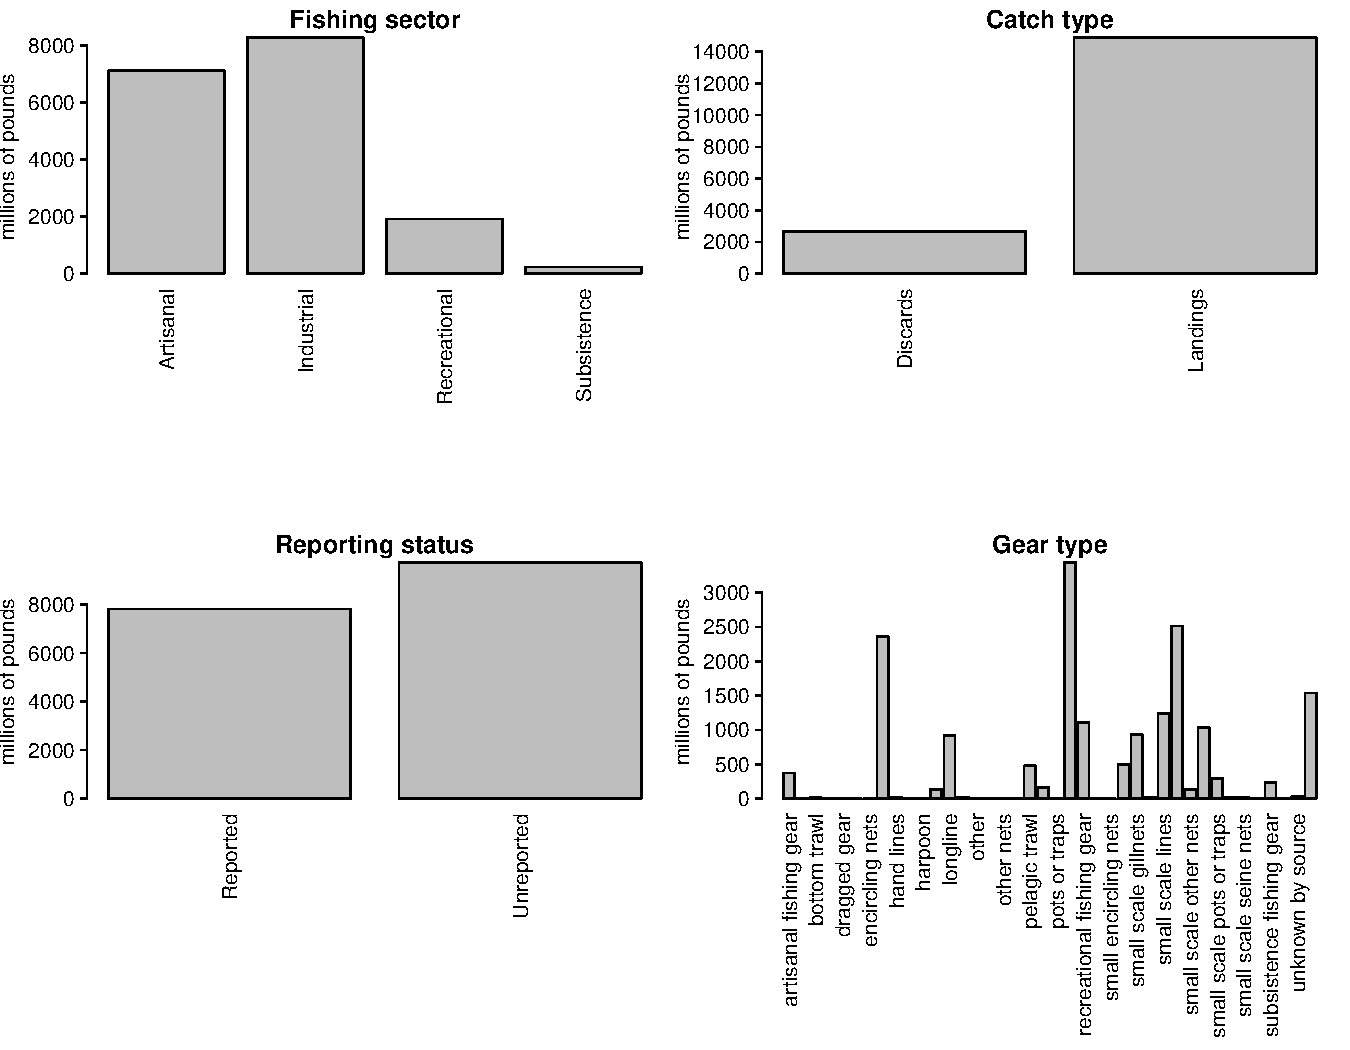
\includegraphics{SAU_EEZs_files/figure-pdf/unnamed-chunk-2-1.pdf}

\begin{Shaded}
\begin{Highlighting}[]
\FunctionTok{round}\NormalTok{(}\FunctionTok{tapply}\NormalTok{(d}\SpecialCharTok{$}\NormalTok{lbs, d}\SpecialCharTok{$}\NormalTok{catch\_type, sum, }\AttributeTok{na.rm =}\NormalTok{ T) }\SpecialCharTok{/} \FunctionTok{sum}\NormalTok{(d}\SpecialCharTok{$}\NormalTok{lbs) }\SpecialCharTok{*} \DecValTok{100}\NormalTok{, }\DecValTok{2}\NormalTok{)   }\CommentTok{\# 15\% are discards}
\end{Highlighting}
\end{Shaded}

\begin{verbatim}
Discards Landings 
   15.18    84.82 
\end{verbatim}

\begin{Shaded}
\begin{Highlighting}[]
\FunctionTok{round}\NormalTok{(}\FunctionTok{tapply}\NormalTok{(d}\SpecialCharTok{$}\NormalTok{lbs, d}\SpecialCharTok{$}\NormalTok{reporting\_status, sum, }\AttributeTok{na.rm =}\NormalTok{ T) }\SpecialCharTok{/} \FunctionTok{sum}\NormalTok{(d}\SpecialCharTok{$}\NormalTok{lbs) }\SpecialCharTok{*} \DecValTok{100}\NormalTok{, }\DecValTok{2}\NormalTok{)  }\CommentTok{\# 55\% are unreported}
\end{Highlighting}
\end{Shaded}

\begin{verbatim}
  Reported Unreported 
     44.52      55.48 
\end{verbatim}

\section{Separating the EEZs by area}\label{separating-the-eezs-by-area}

Now we have to manually assign the different EEZs to respective areas.
We separate the geographical areas within the Atlantic Ocean (North and
South) and lump all other EEZs into ``other oceans.'' This latter
category is largely the Pacific Ocean and to a lesser extent the Indian
Ocean. We remove the high seas catch from this database as it is not
ocean-specific and we have extracted the ocean-specific high seas catch
previously.

\begin{Shaded}
\begin{Highlighting}[]
\CommentTok{\# remove the high seas catch from this database}
\NormalTok{d }\OtherTok{\textless{}{-}}\NormalTok{ d[}\FunctionTok{which}\NormalTok{(d}\SpecialCharTok{$}\NormalTok{area\_type }\SpecialCharTok{!=} \StringTok{"high\_seas"}\NormalTok{), ]   }
\NormalTok{d}\SpecialCharTok{$}\NormalTok{fishing\_entity }\OtherTok{\textless{}{-}} \FunctionTok{as.factor}\NormalTok{(d}\SpecialCharTok{$}\NormalTok{fishing\_entity)}
\NormalTok{d}\SpecialCharTok{$}\NormalTok{fishing\_entity }\OtherTok{\textless{}{-}} \FunctionTok{droplevels}\NormalTok{(d}\SpecialCharTok{$}\NormalTok{fishing\_entity)}
\FunctionTok{table}\NormalTok{(d}\SpecialCharTok{$}\NormalTok{area\_type)  }\CommentTok{\# this should be all "eez"}
\end{Highlighting}
\end{Shaded}

\begin{verbatim}

  eez 
63056 
\end{verbatim}

\begin{Shaded}
\begin{Highlighting}[]
\CommentTok{\# Western Central Atlantic EEZs}
\NormalTok{WCA }\OtherTok{\textless{}{-}} \FunctionTok{c}\NormalTok{(}\StringTok{"Bahamas"}\NormalTok{, }\StringTok{"Barbados"}\NormalTok{, }\StringTok{"Cayman Isl. (UK)"}\NormalTok{, }\StringTok{"Dominica"}\NormalTok{, }\StringTok{"Dominican Republic"}\NormalTok{, }\StringTok{"Grenada"}\NormalTok{, }
         \StringTok{"Aruba (Netherlands)"}\NormalTok{, }\StringTok{"Haiti"}\NormalTok{, }\StringTok{"Guadeloupe  (France)"}\NormalTok{, }\StringTok{"Jamaica"}\NormalTok{, }\StringTok{"Martinique (France)"}\NormalTok{,}
         \StringTok{"Montserrat (UK)"}\NormalTok{, }\StringTok{"Nicaragua (Caribbean)"}\NormalTok{, }\StringTok{"Puerto Rico (USA)"}\NormalTok{, }\StringTok{"Saint Kitts \& Nevis"}\NormalTok{, }
         \StringTok{"Saint Lucia"}\NormalTok{, }\StringTok{"Saint Vincent \& the Grenadines"}\NormalTok{, }\StringTok{"Trinidad \& Tobago"}\NormalTok{, }\StringTok{"US Virgin Isl."}\NormalTok{, }
         \StringTok{"St Barthelemy (France)"}\NormalTok{, }\StringTok{"St Martin (France)"}\NormalTok{, }\StringTok{"Curaçao (Netherlands)"}\NormalTok{, }\StringTok{"Bonaire (Netherlands)"}\NormalTok{,}
         \StringTok{"Saba and Sint Eustatius (Netherlands)"}\NormalTok{, }\StringTok{"Sint Maarten (Netherlands)"}\NormalTok{, }\StringTok{"Honduras (Caribbean)"}\NormalTok{,}
         \StringTok{"Colombia (Caribbean)"}\NormalTok{, }\StringTok{"Mexico (Atlantic)"}\NormalTok{, }\StringTok{"Turks \& Caicos Isl. (UK)"}\NormalTok{, }\StringTok{"Guyana"}\NormalTok{, }\StringTok{"Venezuela"}\NormalTok{,}
         \StringTok{"Antigua \& Barbuda"}\NormalTok{, }\StringTok{"Belize"}\NormalTok{, }\StringTok{"British Virgin Isl. (UK)"}\NormalTok{, }\StringTok{"French Guiana"}\NormalTok{, }\StringTok{"Cuba"}\NormalTok{, }
         \StringTok{"Anguilla (UK)"}\NormalTok{, }\StringTok{"Suriname"}\NormalTok{, }\StringTok{"Costa Rica (Caribbean)"}\NormalTok{, }\StringTok{"Guatemala (Caribbean)"}\NormalTok{, }
         \StringTok{"Panama (Caribbean)"}\NormalTok{, }\StringTok{"Bermuda (UK)"}\NormalTok{, }\StringTok{"Curaçao (Netherlands)"}\NormalTok{) }
           
\CommentTok{\# Brazil}
\NormalTok{Bra }\OtherTok{\textless{}{-}} \FunctionTok{c}\NormalTok{(}\StringTok{"Brazil (mainland)"}\NormalTok{, }\StringTok{"Fernando de Noronha (Brazil)"}\NormalTok{, }
         \StringTok{"St Paul and St. Peter Archipelago (Brazil)"}\NormalTok{)}

\CommentTok{\# Canada}
\NormalTok{Can }\OtherTok{\textless{}{-}}  \FunctionTok{c}\NormalTok{(}\StringTok{"Canada (East Coast)"}\NormalTok{, }\StringTok{"Saint Pierre \& Miquelon (France)"}\NormalTok{)}

\CommentTok{\# United States}
\NormalTok{USA }\OtherTok{\textless{}{-}}  \FunctionTok{c}\NormalTok{(}\StringTok{"USA (East Coast)"}\NormalTok{, }\StringTok{"USA (Gulf of Mexico)"}\NormalTok{)}
           
\CommentTok{\# Northeast Atlantic EEZs}
\NormalTok{NEA }\OtherTok{\textless{}{-}} \FunctionTok{c}\NormalTok{(}\StringTok{"Canary Isl. (Spain)"}\NormalTok{, }\StringTok{"Spain (mainland; Med and Gulf of Cadiz)"}\NormalTok{, }\StringTok{"Spain (Northwest)"}\NormalTok{, }
         \StringTok{"Spain (mainland, Med and Gulf of Cadiz)"}\NormalTok{, }
         \StringTok{"France (Atlantic Coast)"}\NormalTok{, }\StringTok{"Portugal (mainland)"}\NormalTok{, }\StringTok{"Azores Isl. (Portugal)"}\NormalTok{)}
        
\CommentTok{\# Eastern Central Atlantic EEZs}
\NormalTok{ECA }\OtherTok{\textless{}{-}} \FunctionTok{c}\NormalTok{(}\StringTok{"Madeira Isl. (Portugal)"}\NormalTok{, }\StringTok{"Cape Verde"}\NormalTok{, }\StringTok{"Equatorial Guinea"}\NormalTok{, }\StringTok{"Benin"}\NormalTok{, }
          \StringTok{"Sao Tome \& Principe "}\NormalTok{, }\StringTok{"Sao Tome \& Principe"}\NormalTok{, }\StringTok{"Morocco (Central)"}\NormalTok{, }\StringTok{"Ghana"}\NormalTok{, }
          \StringTok{"Côte d\textquotesingle{}Ivoire"}\NormalTok{, }\StringTok{"Côte d\textquotesingle{}Ivoire"}\NormalTok{, }\StringTok{"Guinea"}\NormalTok{, }\StringTok{"Liberia"}\NormalTok{, }\StringTok{"Sierra Leone"}\NormalTok{, }\StringTok{"Nigeria"}\NormalTok{, }\StringTok{"Togo"}\NormalTok{, }
          \StringTok{"Guinea{-}Bissau"}\NormalTok{, }\StringTok{"Senegal"}\NormalTok{, }\StringTok{"Cameroon"}\NormalTok{, }\StringTok{"Gambia"}\NormalTok{, }\StringTok{"Mauritania"}\NormalTok{, }\StringTok{"Morocco (South)"}\NormalTok{, }
          \StringTok{"Gabon"}\NormalTok{, }\StringTok{"Congo; R. of"}\NormalTok{, }\StringTok{"Congo, R. of"}\NormalTok{, }\StringTok{"Congo (ex{-}Zaire)"}\NormalTok{)}

\CommentTok{\# Southeastern Atlantic EEZs}
\NormalTok{SEA }\OtherTok{\textless{}{-}} \FunctionTok{c}\NormalTok{(}\StringTok{"Angola"}\NormalTok{, }\StringTok{"Namibia"}\NormalTok{, }\StringTok{"South Africa (Atlantic and Cape)"}\NormalTok{,  }
           \StringTok{"Ascension Isl. (UK)"}\NormalTok{, }\StringTok{"Saint Helena (UK)"}\NormalTok{, }\StringTok{"Tristan da Cunha Isl. (UK)"}\NormalTok{)}

\CommentTok{\# Southwest Atlantic EEZs}
\NormalTok{SWA }\OtherTok{\textless{}{-}} \FunctionTok{c}\NormalTok{(}\StringTok{"Trindade \& Martim Vaz Isl. (Brazil)"}\NormalTok{, }\StringTok{"Uruguay"}\NormalTok{)}

\CommentTok{\# Mediterranean EEZs}
\NormalTok{Med }\OtherTok{\textless{}{-}} \FunctionTok{c}\NormalTok{(}\StringTok{"Italy (mainland)"}\NormalTok{, }\StringTok{"Libya"}\NormalTok{, }\StringTok{"Malta"}\NormalTok{, }\StringTok{"Syria"}\NormalTok{, }\StringTok{"Sicily (Italy)"}\NormalTok{,}\StringTok{"Sardinia (Italy)"}\NormalTok{, }
         \StringTok{"Balearic Islands (Spain)"}\NormalTok{, }\StringTok{"Cyprus (North)"}\NormalTok{, }\StringTok{"Cyprus (South)"}\NormalTok{, }
         \StringTok{"Gaza Strip"}\NormalTok{, }\StringTok{"Greece (without Crete)"}\NormalTok{, }\StringTok{"Crete (Greece)"}\NormalTok{, }\StringTok{"Lebanon"}\NormalTok{, }
         \StringTok{"Turkey (Mediterranean Sea)"}\NormalTok{, }\StringTok{"Egypt (Mediterranean)"}\NormalTok{, }\StringTok{"Israel (Mediterranean)"}\NormalTok{, }\StringTok{"Tunisia"}\NormalTok{, }
         \StringTok{"Algeria"}\NormalTok{, }\StringTok{"Albania"}\NormalTok{, }\StringTok{"Croatia"}\NormalTok{, }\StringTok{"Montenegro"}\NormalTok{, }\StringTok{"Morocco (Mediterranean)"}\NormalTok{, }
         \StringTok{"France (Mediterranean)"}\NormalTok{, }\StringTok{"Corsica (France)"}\NormalTok{)}

\CommentTok{\# add variable to specify region}
\NormalTok{d}\SpecialCharTok{$}\NormalTok{reg }\OtherTok{\textless{}{-}} \StringTok{"other oceans"}
\NormalTok{d}\SpecialCharTok{$}\NormalTok{reg[}\FunctionTok{which}\NormalTok{(d}\SpecialCharTok{$}\NormalTok{area\_name }\SpecialCharTok{\%in\%}\NormalTok{ WCA)] }\OtherTok{\textless{}{-}} \StringTok{"Western Central Atlantic EEZs"}
\NormalTok{d}\SpecialCharTok{$}\NormalTok{reg[}\FunctionTok{which}\NormalTok{(d}\SpecialCharTok{$}\NormalTok{area\_name }\SpecialCharTok{\%in\%}\NormalTok{ Bra)] }\OtherTok{\textless{}{-}} \StringTok{"Brazil EEZ"}
\NormalTok{d}\SpecialCharTok{$}\NormalTok{reg[}\FunctionTok{which}\NormalTok{(d}\SpecialCharTok{$}\NormalTok{area\_name }\SpecialCharTok{\%in\%}\NormalTok{ Can)] }\OtherTok{\textless{}{-}} \StringTok{"Canadian EEZ"}
\NormalTok{d}\SpecialCharTok{$}\NormalTok{reg[}\FunctionTok{which}\NormalTok{(d}\SpecialCharTok{$}\NormalTok{area\_name }\SpecialCharTok{\%in\%}\NormalTok{ USA)] }\OtherTok{\textless{}{-}} \StringTok{"United States EEZ"}
\NormalTok{d}\SpecialCharTok{$}\NormalTok{reg[}\FunctionTok{which}\NormalTok{(d}\SpecialCharTok{$}\NormalTok{area\_name }\SpecialCharTok{\%in\%}\NormalTok{ NEA)] }\OtherTok{\textless{}{-}} \StringTok{"Northeast Atlantic EEZs"}
\NormalTok{d}\SpecialCharTok{$}\NormalTok{reg[}\FunctionTok{which}\NormalTok{(d}\SpecialCharTok{$}\NormalTok{area\_name }\SpecialCharTok{\%in\%}\NormalTok{ ECA)] }\OtherTok{\textless{}{-}} \StringTok{"Eastern Central Atlantic EEZs"}
\NormalTok{d}\SpecialCharTok{$}\NormalTok{reg[}\FunctionTok{which}\NormalTok{(d}\SpecialCharTok{$}\NormalTok{area\_name }\SpecialCharTok{\%in\%}\NormalTok{ SEA)] }\OtherTok{\textless{}{-}} \StringTok{"Southeast Atlantic EEZs"}
\NormalTok{d}\SpecialCharTok{$}\NormalTok{reg[}\FunctionTok{which}\NormalTok{(d}\SpecialCharTok{$}\NormalTok{area\_name }\SpecialCharTok{\%in\%}\NormalTok{ SWA)] }\OtherTok{\textless{}{-}} \StringTok{"Southwest Atlantic EEZs"}
\NormalTok{d}\SpecialCharTok{$}\NormalTok{reg[}\FunctionTok{which}\NormalTok{(d}\SpecialCharTok{$}\NormalTok{area\_name }\SpecialCharTok{\%in\%}\NormalTok{ Med)] }\OtherTok{\textless{}{-}} \StringTok{"Mediterranean Sea EEZs"}
\end{Highlighting}
\end{Shaded}

Now we will check that we have classified the regions correctly.

\begin{Shaded}
\begin{Highlighting}[]
\CommentTok{\# check region designation }
\NormalTok{othlis }\OtherTok{\textless{}{-}} \FunctionTok{unique}\NormalTok{(d}\SpecialCharTok{$}\NormalTok{area\_name[}\FunctionTok{which}\NormalTok{(d}\SpecialCharTok{$}\NormalTok{reg }\SpecialCharTok{==} \StringTok{"other oceans"}\NormalTok{)])}
\FunctionTok{print}\NormalTok{(}\StringTok{"EEZs of all other oceans: "}\NormalTok{)}
\end{Highlighting}
\end{Shaded}

\begin{verbatim}
[1] "EEZs of all other oceans: "
\end{verbatim}

\begin{Shaded}
\begin{Highlighting}[]
\NormalTok{othlis}
\end{Highlighting}
\end{Shaded}

\begin{verbatim}
  [1] "Australia"                          "China"                             
  [3] "Taiwan"                             "Mayotte (France)"                  
  [5] "French Polynesia"                   "Hong Kong (China)"                 
  [7] "Andaman & Nicobar Isl. (India)"     "Indonesia (Eastern)"               
  [9] "Japan (main islands)"               "Japan (Daito Islands)"             
 [11] "Korea (South)"                      "Hawaii Northwest Islands (USA)"    
 [13] "Nauru"                              "Niue (New Zealand)"                
 [15] "Northern Marianas (USA)"            "Micronesia (Federated States of)"  
 [17] "Marshall Isl."                      "Palau"                             
 [19] "Pakistan"                           "Papua New Guinea"                  
 [21] "Philippines"                        "Seychelles"                        
 [23] "Viet Nam"                           "Tokelau (New Zealand)"             
 [25] "Tonga"                              "Hawaii Main Islands (USA)"         
 [27] "USA (West Coast)"                   "Wake Isl. (USA)"                   
 [29] "Wallis & Futuna Isl. (France)"      "Samoa"                             
 [31] "Guatemala (Pacific)"                "Kiribati (Gilbert Islands)"        
 [33] "Mexico (Pacific)"                   "Japan (Ogasawara Islands)"         
 [35] "Korea (North, Yellow Sea)"          "Korea (North, Sea of Japan)"       
 [37] "Mauritius"                          "Solomon Isl."                      
 [39] "Christmas Isl. (Australia)"         "Johnston Atoll (USA)"              
 [41] "Timor Leste"                        "Palmyra Atoll & Kingman Reef (USA)"
 [43] "Jarvis Isl. (USA)"                  "Howland & Baker Isl. (USA)"        
 [45] "Indonesia (Central)"                "Indonesia (Indian Ocean)"          
 [47] "Kiribati (Line Islands)"            "Kiribati (Phoenix Islands)"        
 [49] "New Caledonia (France)"             "Vanuatu"                           
 [51] "Lord Howe Isl. (Australia)"         "Myanmar"                           
 [53] "Ecuador (mainland)"                 "El Salvador"                       
 [55] "Fiji"                               "Malaysia (Peninsula West)"         
 [57] "Norfolk Isl. (Australia)"           "Peru"                              
 [59] "Pitcairn (UK)"                      "Colombia (Pacific)"                
 [61] "Costa Rica (Pacific)"               "Nicaragua (Pacific)"               
 [63] "Panama (Pacific)"                   "Thailand (Andaman Sea)"            
 [65] "Thailand (Gulf of Thailand)"        "Cook Islands"                      
 [67] "Kermadec Isl. (New Zealand)"        "Tuvalu"                            
 [69] "Honduras (Pacific)"                 "American Samoa"                    
 [71] "Galapagos Isl. (Ecuador)"           "New Zealand"                       
 [73] "Brunei Darussalam"                  "Malaysia (Sabah)"                  
 [75] "Malaysia (Sarawak)"                 "Guam (USA)"                        
 [77] "Clipperton Isl. (France)"           "South Africa (Indian Ocean Coast)" 
 [79] "Singapore"                          "Easter Isl. (Chile)"               
 [81] "Madagascar"                         "Réunion (France)"                  
 [83] "Chagos Archipelago (UK)"            "Comoros Isl."                      
 [85] "Mozambique Channel Isl. (France)"   "Kenya"                             
 [87] "Mozambique"                         "Somalia"                           
 [89] "Tanzania"                           "Glorieuse Islands (France)"        
 [91] "Yemen (Socotra)"                    "Oman"                              
 [93] "St Paul & Amsterdam Isl. (France)"  "Iran (Sea of Oman)"                
 [95] "Desventuradas Isl. (Chile)"         "India (mainland)"                  
 [97] "Maldives"                           "Tromelin Isl. (France)"            
 [99] "Cambodia"                           "Sri Lanka"                         
[101] "Malaysia (Peninsula East)"          "Bangladesh"                        
\end{verbatim}

\begin{Shaded}
\begin{Highlighting}[]
\FunctionTok{print}\NormalTok{(}\StringTok{"U.S. EEZs outside the Atlantic Ocean: "}\NormalTok{)}
\end{Highlighting}
\end{Shaded}

\begin{verbatim}
[1] "U.S. EEZs outside the Atlantic Ocean: "
\end{verbatim}

\begin{Shaded}
\begin{Highlighting}[]
\NormalTok{othlis[}\FunctionTok{grep}\NormalTok{(}\StringTok{"USA"}\NormalTok{, othlis)]}
\end{Highlighting}
\end{Shaded}

\begin{verbatim}
 [1] "Hawaii Northwest Islands (USA)"     "Northern Marianas (USA)"           
 [3] "Hawaii Main Islands (USA)"          "USA (West Coast)"                  
 [5] "Wake Isl. (USA)"                    "Johnston Atoll (USA)"              
 [7] "Palmyra Atoll & Kingman Reef (USA)" "Jarvis Isl. (USA)"                 
 [9] "Howland & Baker Isl. (USA)"         "Guam (USA)"                        
\end{verbatim}

\begin{Shaded}
\begin{Highlighting}[]
\FunctionTok{print}\NormalTok{(}\StringTok{"French EEZs outside the Atlantic Ocean: "}\NormalTok{)}
\end{Highlighting}
\end{Shaded}

\begin{verbatim}
[1] "French EEZs outside the Atlantic Ocean: "
\end{verbatim}

\begin{Shaded}
\begin{Highlighting}[]
\NormalTok{othlis[}\FunctionTok{grep}\NormalTok{(}\StringTok{"France"}\NormalTok{, othlis)]}
\end{Highlighting}
\end{Shaded}

\begin{verbatim}
[1] "Mayotte (France)"                  "Wallis & Futuna Isl. (France)"    
[3] "New Caledonia (France)"            "Clipperton Isl. (France)"         
[5] "Réunion (France)"                  "Mozambique Channel Isl. (France)" 
[7] "Glorieuse Islands (France)"        "St Paul & Amsterdam Isl. (France)"
[9] "Tromelin Isl. (France)"           
\end{verbatim}

\begin{Shaded}
\begin{Highlighting}[]
\FunctionTok{unique}\NormalTok{(d}\SpecialCharTok{$}\NormalTok{area\_name[}\FunctionTok{which}\NormalTok{(d}\SpecialCharTok{$}\NormalTok{reg }\SpecialCharTok{==} \StringTok{"Western Central Atlantic EEZs"}\NormalTok{)])   }\CommentTok{\# Western Central EEZs:}
\end{Highlighting}
\end{Shaded}

\begin{verbatim}
 [1] "Bahamas"                              
 [2] "Barbados"                             
 [3] "Bermuda (UK)"                         
 [4] "Cayman Isl. (UK)"                     
 [5] "Dominica"                             
 [6] "Dominican Republic"                   
 [7] "Grenada"                              
 [8] "Guadeloupe  (France)"                 
 [9] "Haiti"                                
[10] "Jamaica"                              
[11] "Martinique (France)"                  
[12] "Montserrat (UK)"                      
[13] "Puerto Rico (USA)"                    
[14] "Saint Kitts & Nevis"                  
[15] "Saint Lucia"                          
[16] "Saint Vincent & the Grenadines"       
[17] "Trinidad & Tobago"                    
[18] "US Virgin Isl."                       
[19] "St Barthelemy (France)"               
[20] "St Martin (France)"                   
[21] "Curaçao (Netherlands)"                
[22] "Bonaire (Netherlands)"                
[23] "Saba and Sint Eustatius (Netherlands)"
[24] "Sint Maarten (Netherlands)"           
[25] "Honduras (Caribbean)"                 
[26] "Colombia (Caribbean)"                 
[27] "Mexico (Atlantic)"                    
[28] "Turks & Caicos Isl. (UK)"             
[29] "Costa Rica (Caribbean)"               
[30] "Panama (Caribbean)"                   
[31] "Antigua & Barbuda"                    
[32] "Belize"                               
[33] "British Virgin Isl. (UK)"             
[34] "Cuba"                                 
[35] "French Guiana"                        
[36] "Guyana"                               
[37] "Anguilla (UK)"                        
[38] "Suriname"                             
[39] "Venezuela"                            
[40] "Guatemala (Caribbean)"                
[41] "Aruba (Netherlands)"                  
[42] "Nicaragua (Caribbean)"                
\end{verbatim}

\begin{Shaded}
\begin{Highlighting}[]
\FunctionTok{unique}\NormalTok{(d}\SpecialCharTok{$}\NormalTok{area\_name[}\FunctionTok{which}\NormalTok{(d}\SpecialCharTok{$}\NormalTok{reg }\SpecialCharTok{==} \StringTok{"Brazil EEZ"}\NormalTok{)])   }\CommentTok{\# Brazil EEZs:}
\end{Highlighting}
\end{Shaded}

\begin{verbatim}
[1] "Brazil (mainland)"                         
[2] "Fernando de Noronha (Brazil)"              
[3] "St Paul and St. Peter Archipelago (Brazil)"
\end{verbatim}

\begin{Shaded}
\begin{Highlighting}[]
\FunctionTok{unique}\NormalTok{(d}\SpecialCharTok{$}\NormalTok{area\_name[}\FunctionTok{which}\NormalTok{(d}\SpecialCharTok{$}\NormalTok{reg }\SpecialCharTok{==} \StringTok{"Canadian EEZ"}\NormalTok{)])   }\CommentTok{\# Canadian EEZs:}
\end{Highlighting}
\end{Shaded}

\begin{verbatim}
[1] "Canada (East Coast)"              "Saint Pierre & Miquelon (France)"
\end{verbatim}

\begin{Shaded}
\begin{Highlighting}[]
\FunctionTok{unique}\NormalTok{(d}\SpecialCharTok{$}\NormalTok{area\_name[}\FunctionTok{which}\NormalTok{(d}\SpecialCharTok{$}\NormalTok{reg }\SpecialCharTok{==} \StringTok{"United States EEZ"}\NormalTok{)])  }\CommentTok{\# United States EEZs:}
\end{Highlighting}
\end{Shaded}

\begin{verbatim}
[1] "USA (East Coast)"     "USA (Gulf of Mexico)"
\end{verbatim}

\begin{Shaded}
\begin{Highlighting}[]
\FunctionTok{unique}\NormalTok{(d}\SpecialCharTok{$}\NormalTok{area\_name[}\FunctionTok{which}\NormalTok{(d}\SpecialCharTok{$}\NormalTok{reg }\SpecialCharTok{==} \StringTok{"Northeast Atlantic EEZs"}\NormalTok{)])   }\CommentTok{\# Northeast Atlantic EEZs:}
\end{Highlighting}
\end{Shaded}

\begin{verbatim}
[1] "Azores Isl. (Portugal)"                 
[2] "Spain (mainland, Med and Gulf of Cadiz)"
[3] "Canary Isl. (Spain)"                    
[4] "Portugal (mainland)"                    
[5] "France (Atlantic Coast)"                
[6] "Spain (Northwest)"                      
\end{verbatim}

\begin{Shaded}
\begin{Highlighting}[]
\FunctionTok{unique}\NormalTok{(d}\SpecialCharTok{$}\NormalTok{area\_name[}\FunctionTok{which}\NormalTok{(d}\SpecialCharTok{$}\NormalTok{reg }\SpecialCharTok{==} \StringTok{"Eastern Central Atlantic EEZs"}\NormalTok{)])   }\CommentTok{\# Eastern Central Atlantic EEZs:}
\end{Highlighting}
\end{Shaded}

\begin{verbatim}
 [1] "Cape Verde"              "Equatorial Guinea"      
 [3] "Sao Tome & Principe"     "Madeira Isl. (Portugal)"
 [5] "Togo"                    "Ghana"                  
 [7] "Guinea"                  "Liberia"                
 [9] "Guinea-Bissau"           "Senegal"                
[11] "Sierra Leone"            "Morocco (Central)"      
[13] "Morocco (South)"         "Côte d'Ivoire"          
[15] "Gabon"                   "Benin"                  
[17] "Gambia"                  "Mauritania"             
[19] "Nigeria"                 "Cameroon"               
[21] "Congo, R. of"            "Congo (ex-Zaire)"       
\end{verbatim}

\begin{Shaded}
\begin{Highlighting}[]
\FunctionTok{unique}\NormalTok{(d}\SpecialCharTok{$}\NormalTok{area\_name[}\FunctionTok{which}\NormalTok{(d}\SpecialCharTok{$}\NormalTok{reg }\SpecialCharTok{==} \StringTok{"Southeast Atlantic EEZs"}\NormalTok{)])   }\CommentTok{\# Southeast Atlantic EEZs:}
\end{Highlighting}
\end{Shaded}

\begin{verbatim}
[1] "Ascension Isl. (UK)"              "South Africa (Atlantic and Cape)"
[3] "Saint Helena (UK)"                "Angola"                          
[5] "Namibia"                          "Tristan da Cunha Isl. (UK)"      
\end{verbatim}

\begin{Shaded}
\begin{Highlighting}[]
\FunctionTok{unique}\NormalTok{(d}\SpecialCharTok{$}\NormalTok{area\_name[}\FunctionTok{which}\NormalTok{(d}\SpecialCharTok{$}\NormalTok{reg }\SpecialCharTok{==} \StringTok{"Southwest Atlantic EEZs"}\NormalTok{)])   }\CommentTok{\# Southwest Atlantic EEZs:}
\end{Highlighting}
\end{Shaded}

\begin{verbatim}
[1] "Trindade & Martim Vaz Isl. (Brazil)" "Uruguay"                            
\end{verbatim}

\begin{Shaded}
\begin{Highlighting}[]
\FunctionTok{unique}\NormalTok{(d}\SpecialCharTok{$}\NormalTok{area\_name[}\FunctionTok{which}\NormalTok{(d}\SpecialCharTok{$}\NormalTok{reg }\SpecialCharTok{==} \StringTok{"Mediterranean Sea EEZs"}\NormalTok{)])   }\CommentTok{\# Mediterranean Sea EEZs:}
\end{Highlighting}
\end{Shaded}

\begin{verbatim}
 [1] "Italy (mainland)"         "Libya"                   
 [3] "Malta"                    "Syria"                   
 [5] "Sicily (Italy)"           "Sardinia (Italy)"        
 [7] "Balearic Islands (Spain)" "Tunisia"                 
 [9] "Algeria"                  "Morocco (Mediterranean)" 
[11] "France (Mediterranean)"   "Corsica (France)"        
[13] "Croatia"                  "Lebanon"                 
[15] "Albania"                  "Greece (without Crete)"  
[17] "Crete (Greece)"           "Cyprus (South)"          
\end{verbatim}

\section{Summarize catch by regional
EEZs}\label{summarize-catch-by-regional-eezs}

Now we summarize the catch by region by grouping the catch across the
EEZs by region. We save these data for later analysis, and move on to
analyzing only the Western Central and Northwest Atlantic jurisdictions.

\begin{Shaded}
\begin{Highlighting}[]
\CommentTok{\# summarize EEZ catch by region}
\NormalTok{tab }\OtherTok{\textless{}{-}} \FunctionTok{tapply}\NormalTok{(d}\SpecialCharTok{$}\NormalTok{lbs, }\FunctionTok{list}\NormalTok{(d}\SpecialCharTok{$}\NormalTok{year, d}\SpecialCharTok{$}\NormalTok{reg), sum, }\AttributeTok{na.rm =}\NormalTok{ T)}
\FunctionTok{write.csv}\NormalTok{(}\FunctionTok{data.frame}\NormalTok{(tab), }\AttributeTok{file =} \StringTok{"data/outputs/intl\_catches\_allAtlantic.csv"}\NormalTok{, }\AttributeTok{row.names =}\NormalTok{ T)}

\NormalTok{dwest }\OtherTok{\textless{}{-}}\NormalTok{ d[}\FunctionTok{which}\NormalTok{(d}\SpecialCharTok{$}\NormalTok{reg }\SpecialCharTok{==} \StringTok{"Canadian EEZ"} \SpecialCharTok{|}\NormalTok{ d}\SpecialCharTok{$}\NormalTok{reg }\SpecialCharTok{==} \StringTok{"Western Central Atlantic EEZs"}\NormalTok{), ]}
\FunctionTok{save}\NormalTok{(dwest, }\AttributeTok{file =} \StringTok{"data/outputs/SAU\_EEZs\_WCA.RData"}\NormalTok{)}

\NormalTok{tab }\OtherTok{\textless{}{-}} \FunctionTok{tapply}\NormalTok{(dwest}\SpecialCharTok{$}\NormalTok{lbs, }\FunctionTok{list}\NormalTok{(dwest}\SpecialCharTok{$}\NormalTok{year, dwest}\SpecialCharTok{$}\NormalTok{area\_name), sum, }\AttributeTok{na.rm =}\NormalTok{ T)}

\CommentTok{\# eight countries are responsible for vast majority of catch with total landings across all years exceeding 20M pounds}
\FunctionTok{par}\NormalTok{(}\AttributeTok{mar =} \FunctionTok{c}\NormalTok{(}\DecValTok{17}\NormalTok{, }\DecValTok{4}\NormalTok{, }\DecValTok{3}\NormalTok{, }\DecValTok{1}\NormalTok{))}
\FunctionTok{barplot}\NormalTok{(}\FunctionTok{sort}\NormalTok{(}\FunctionTok{colSums}\NormalTok{(tab, }\AttributeTok{na.rm =}\NormalTok{ T)}\SpecialCharTok{/}\DecValTok{10}\SpecialCharTok{\^{}}\DecValTok{6}\NormalTok{, }\AttributeTok{decreasing =}\NormalTok{ T), }\AttributeTok{horiz =}\NormalTok{ F, }\AttributeTok{las =} \DecValTok{2}\NormalTok{,}
        \AttributeTok{main =} \StringTok{"Total dolphin catch (1950 {-} 2022) in the Western Atlantic, by EEZ"}\NormalTok{, }
        \AttributeTok{ylab =} \StringTok{"total catch (millions of pounds)"}\NormalTok{)}
\end{Highlighting}
\end{Shaded}

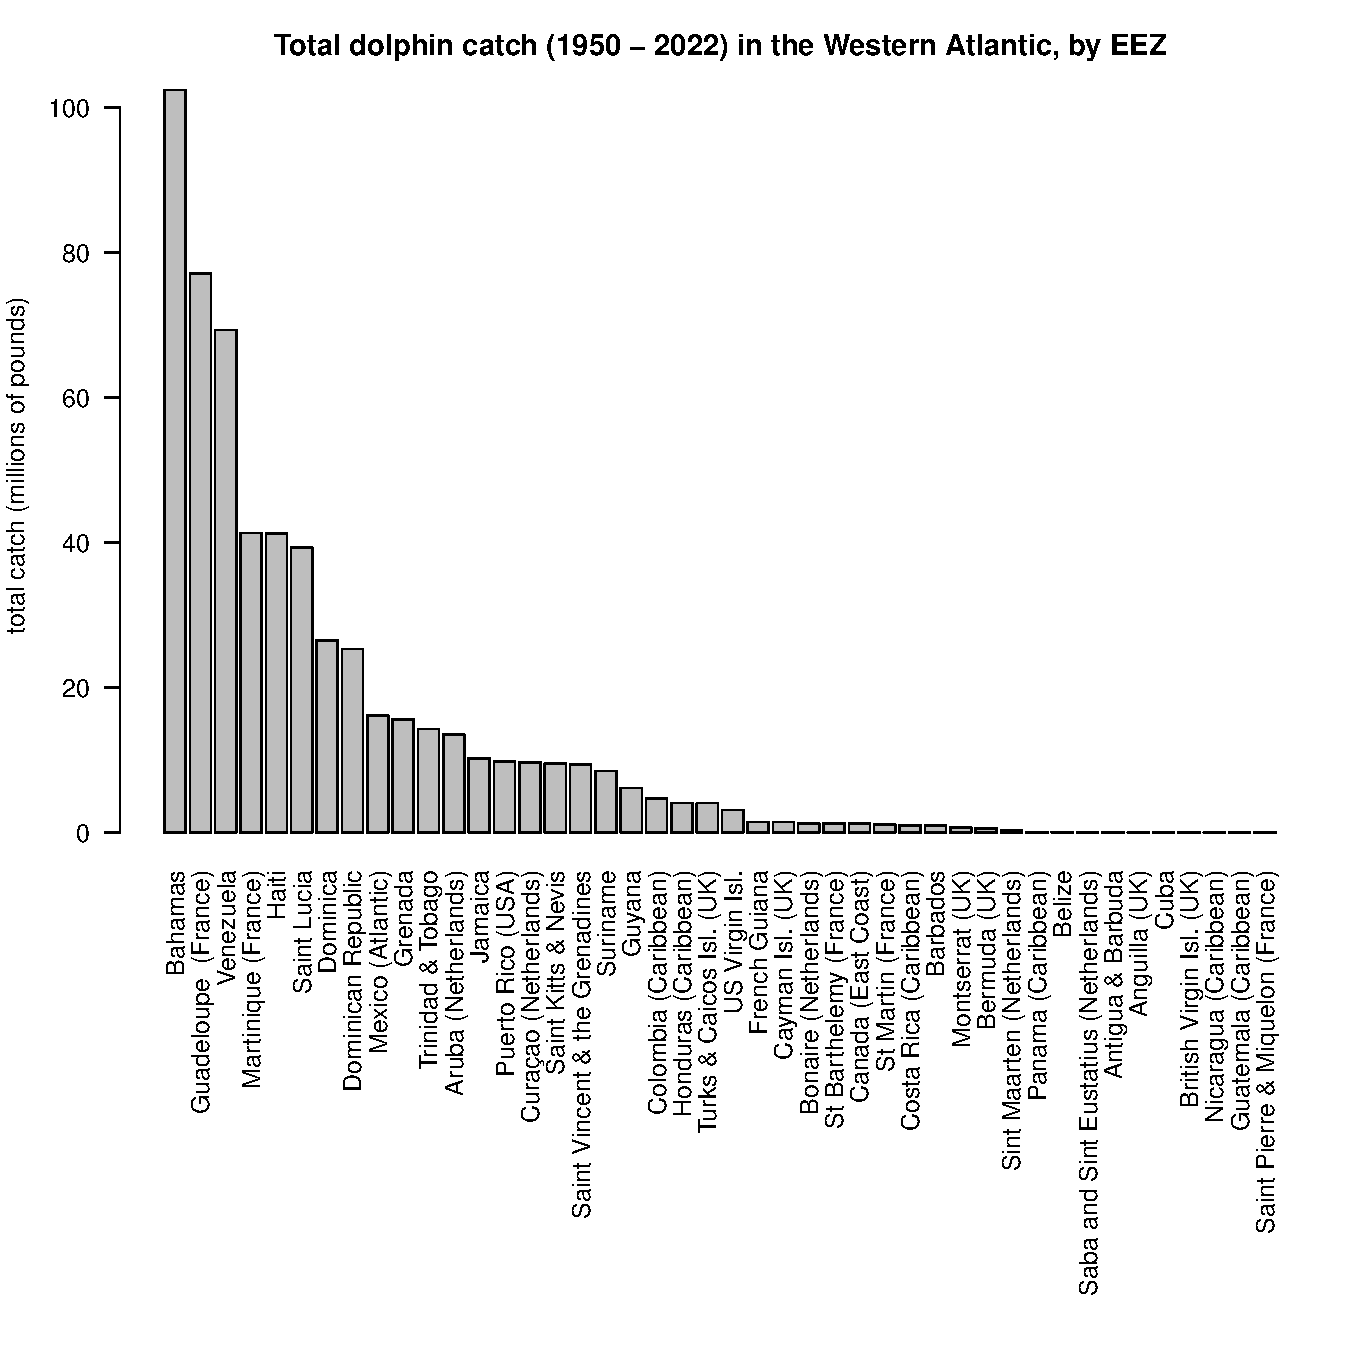
\includegraphics{SAU_EEZs_files/figure-pdf/unnamed-chunk-5-1.pdf}

Note that Bermuda is actually in the NCA region and not the Greater
Caribbean region. However, its catches constitute 0.1\% of the total
catch which is essentially negligible, and to avoid complicating the
operating model and code unnecessarily we will leave those catches
accounted for in the CAR region.

\begin{Shaded}
\begin{Highlighting}[]
\FunctionTok{round}\NormalTok{(}\FunctionTok{colSums}\NormalTok{(tab, }\AttributeTok{na.rm =}\NormalTok{ T)[}\DecValTok{7}\NormalTok{] }\SpecialCharTok{/} \FunctionTok{sum}\NormalTok{(}\FunctionTok{colSums}\NormalTok{(tab, }\AttributeTok{na.rm =}\NormalTok{ T), }\AttributeTok{na.rm =}\NormalTok{ T) }\SpecialCharTok{*} \DecValTok{100}\NormalTok{, }\DecValTok{2}\NormalTok{)}
\end{Highlighting}
\end{Shaded}

\begin{verbatim}
Bermuda (UK) 
         0.1 
\end{verbatim}

\begin{Shaded}
\begin{Highlighting}[]
\NormalTok{lis }\OtherTok{\textless{}{-}} \FunctionTok{names}\NormalTok{(}\FunctionTok{sort}\NormalTok{(}\FunctionTok{colSums}\NormalTok{(tab, }\AttributeTok{na.rm =}\NormalTok{ T), }\AttributeTok{decreasing =}\NormalTok{ T)[}\DecValTok{1}\SpecialCharTok{:}\DecValTok{8}\NormalTok{]) }\CommentTok{\# list of top 8 jurisdictions}
\NormalTok{tab1 }\OtherTok{\textless{}{-}}\NormalTok{ tab[, }\FunctionTok{colnames}\NormalTok{(tab) }\SpecialCharTok{\%in\%}\NormalTok{ lis]}

\FunctionTok{par}\NormalTok{(}\AttributeTok{mar =} \FunctionTok{c}\NormalTok{(}\DecValTok{3}\NormalTok{, }\DecValTok{5}\NormalTok{, }\DecValTok{3}\NormalTok{, }\DecValTok{1}\NormalTok{))}
\FunctionTok{matplot}\NormalTok{(}\FunctionTok{rownames}\NormalTok{(tab1), tab1}\SpecialCharTok{/}\DecValTok{10}\SpecialCharTok{\^{}}\DecValTok{6}\NormalTok{, }\AttributeTok{las =} \DecValTok{2}\NormalTok{, }\AttributeTok{type =} \StringTok{"l"}\NormalTok{, }\AttributeTok{lty =} \DecValTok{1}\NormalTok{, }\AttributeTok{lwd =} \DecValTok{2}\NormalTok{, }\AttributeTok{pch =} \DecValTok{19}\NormalTok{, }\AttributeTok{col =} \DecValTok{1}\SpecialCharTok{:}\DecValTok{8}\NormalTok{,}
        \AttributeTok{xlab =} \StringTok{""}\NormalTok{, }\AttributeTok{ylab =} \StringTok{"total catch (millions of pounds)"}\NormalTok{, }\AttributeTok{axes =}\NormalTok{ F, }
        \AttributeTok{main =} \StringTok{"Total dolphinfish catches in Caribbean EEZs (top 8 jurisdictions)"}\NormalTok{)}
\FunctionTok{axis}\NormalTok{(}\DecValTok{1}\NormalTok{, }\AttributeTok{at =} \FunctionTok{seq}\NormalTok{(}\DecValTok{1950}\NormalTok{, }\DecValTok{2020}\NormalTok{, }\DecValTok{5}\NormalTok{)); }\FunctionTok{axis}\NormalTok{(}\DecValTok{2}\NormalTok{, }\AttributeTok{las =} \DecValTok{2}\NormalTok{); }\FunctionTok{box}\NormalTok{()}
\FunctionTok{legend}\NormalTok{(}\StringTok{"topleft"}\NormalTok{, }\FunctionTok{colnames}\NormalTok{(tab1), }\AttributeTok{col =} \DecValTok{1}\SpecialCharTok{:}\DecValTok{8}\NormalTok{, }\AttributeTok{lty =} \DecValTok{1}\NormalTok{, }\AttributeTok{lwd =} \DecValTok{3}\NormalTok{, }\AttributeTok{bty =} \StringTok{"n"}\NormalTok{, }\AttributeTok{title =} \StringTok{"Fishing area name"}\NormalTok{)}
\end{Highlighting}
\end{Shaded}

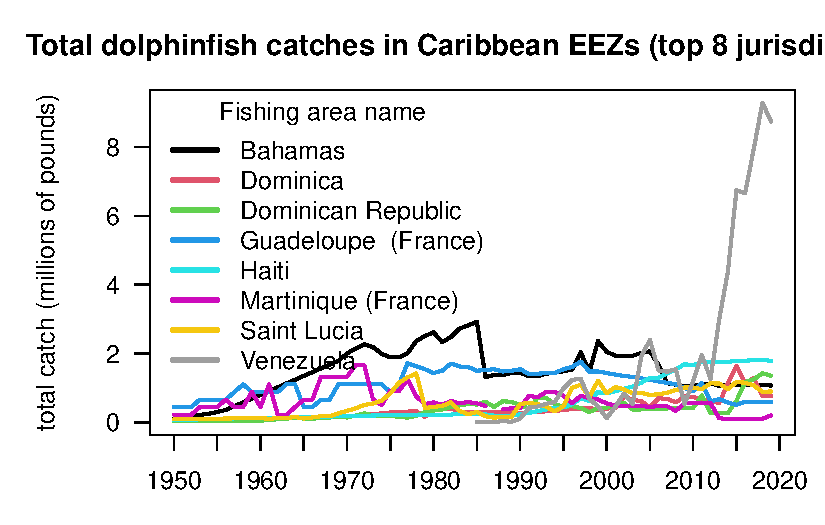
\includegraphics{SAU_EEZs_files/figure-pdf/unnamed-chunk-6-1.pdf}

Note the rapid eight-fold increase in catches listed within the
Venezuelan EEZ which occurs from 2013 - 2019. This increase is
responsible for a rapid increase in estimated international catches
within the Western Atlantic.

\section{Look at Venezuela catches in
detail}\label{look-at-venezuela-catches-in-detail}

The figures above indicate that the database shows a rapid increase in
international catches within the Western Atlantic, driven by a sudden
increase in catches reported within Sea Around Us database within the
Venezuelan EEZ. We investigate these catches in detail, as it seems odd
that a relatively small fleet from a single country would be able to
ramp up effort so rapidly. Data can be downloaded on a country-specific
basis, the catches by taxon in the waters of Venezuela are accessed
\href{https://www.seaaroundus.org/data/\#/eez/862?chart=catch-chart&dimension=taxon&measure=tonnage&limit=10}{here}.

\begin{Shaded}
\begin{Highlighting}[]
\FunctionTok{rm}\NormalTok{(}\AttributeTok{list =} \FunctionTok{ls}\NormalTok{())  }\CommentTok{\# clear the workspace}

\CommentTok{\# download the data for waters of Venezuela}
\NormalTok{ven }\OtherTok{\textless{}{-}} \FunctionTok{read.csv}\NormalTok{(}\StringTok{"data/SAU/SAU EEZ 862 v50{-}1.csv"}\NormalTok{)  }

\CommentTok{\# subset dolphinfish from the data}
\NormalTok{v }\OtherTok{\textless{}{-}}\NormalTok{ ven[}\FunctionTok{which}\NormalTok{(ven}\SpecialCharTok{$}\NormalTok{common\_name }\SpecialCharTok{==} \StringTok{"Common dolphinfish"}\NormalTok{), ]}

\CommentTok{\#apply(v[1:13], 2, table)}

\CommentTok{\#convert to pounds}
\NormalTok{v}\SpecialCharTok{$}\NormalTok{pounds }\OtherTok{\textless{}{-}}\NormalTok{ v}\SpecialCharTok{$}\NormalTok{tonnes }\SpecialCharTok{*} \DecValTok{1000} \SpecialCharTok{*} \FloatTok{2.20462}

\CommentTok{\# look at the characteristics of the data}
\FunctionTok{par}\NormalTok{(}\AttributeTok{mar =} \FunctionTok{c}\NormalTok{(}\DecValTok{5}\NormalTok{, }\DecValTok{10}\NormalTok{, }\DecValTok{1}\NormalTok{, }\DecValTok{1}\NormalTok{), }\AttributeTok{mfrow =} \FunctionTok{c}\NormalTok{(}\DecValTok{3}\NormalTok{, }\DecValTok{2}\NormalTok{), }\AttributeTok{mex =} \FloatTok{0.9}\NormalTok{)}
\CommentTok{\#barplot(tapply(v$pounds/10\^{}6, v$area\_name, sum, na.rm = T), las = 2, xlab = "millions of pounds", main = "Area name", horiz = T)}
\CommentTok{\#barplot(tapply(v$pounds/10\^{}6, v$area\_type, sum, na.rm = T), las = 2, xlab = "millions of pounds", main = "Area type", horiz = T)}
\FunctionTok{barplot}\NormalTok{(}\FunctionTok{tapply}\NormalTok{(v}\SpecialCharTok{$}\NormalTok{pounds}\SpecialCharTok{/}\DecValTok{10}\SpecialCharTok{\^{}}\DecValTok{6}\NormalTok{, v}\SpecialCharTok{$}\NormalTok{year, sum, }\AttributeTok{na.rm =}\NormalTok{ T), }\AttributeTok{las =} \DecValTok{2}\NormalTok{, }\AttributeTok{xlab =} \StringTok{"millions of pounds"}\NormalTok{, }\AttributeTok{main =} \StringTok{"Year"}\NormalTok{, }\AttributeTok{horiz =}\NormalTok{ T)}
\FunctionTok{barplot}\NormalTok{(}\FunctionTok{tapply}\NormalTok{(v}\SpecialCharTok{$}\NormalTok{pounds}\SpecialCharTok{/}\DecValTok{10}\SpecialCharTok{\^{}}\DecValTok{6}\NormalTok{, v}\SpecialCharTok{$}\NormalTok{fishing\_entity, sum, }\AttributeTok{na.rm =}\NormalTok{ T), }\AttributeTok{las =} \DecValTok{2}\NormalTok{, }\AttributeTok{xlab =} \StringTok{"millions of pounds"}\NormalTok{, }\AttributeTok{main =} \StringTok{"Fishing entity"}\NormalTok{, }\AttributeTok{horiz =}\NormalTok{ T)}
\FunctionTok{barplot}\NormalTok{(}\FunctionTok{tapply}\NormalTok{(v}\SpecialCharTok{$}\NormalTok{pounds}\SpecialCharTok{/}\DecValTok{10}\SpecialCharTok{\^{}}\DecValTok{6}\NormalTok{, v}\SpecialCharTok{$}\NormalTok{fishing\_sector, sum, }\AttributeTok{na.rm =}\NormalTok{ T), }\AttributeTok{las =} \DecValTok{2}\NormalTok{, }\AttributeTok{xlab =} \StringTok{"millions of pounds"}\NormalTok{, }\AttributeTok{main =} \StringTok{"Fishing sector"}\NormalTok{, }\AttributeTok{horiz =}\NormalTok{ T)}
\FunctionTok{barplot}\NormalTok{(}\FunctionTok{tapply}\NormalTok{(v}\SpecialCharTok{$}\NormalTok{pounds}\SpecialCharTok{/}\DecValTok{10}\SpecialCharTok{\^{}}\DecValTok{6}\NormalTok{, v}\SpecialCharTok{$}\NormalTok{catch\_type, sum, }\AttributeTok{na.rm =}\NormalTok{ T), }\AttributeTok{las =} \DecValTok{2}\NormalTok{, }\AttributeTok{xlab =} \StringTok{"millions of pounds"}\NormalTok{, }\AttributeTok{main =} \StringTok{"Catch type"}\NormalTok{, }\AttributeTok{horiz =}\NormalTok{ T)}
\FunctionTok{barplot}\NormalTok{(}\FunctionTok{tapply}\NormalTok{(v}\SpecialCharTok{$}\NormalTok{pounds}\SpecialCharTok{/}\DecValTok{10}\SpecialCharTok{\^{}}\DecValTok{6}\NormalTok{, v}\SpecialCharTok{$}\NormalTok{reporting\_status, sum, }\AttributeTok{na.rm =}\NormalTok{ T), }\AttributeTok{las =} \DecValTok{2}\NormalTok{, }\AttributeTok{xlab =} \StringTok{"millions of pounds"}\NormalTok{, }\AttributeTok{main =} \StringTok{"Reporting status"}\NormalTok{, }\AttributeTok{horiz =}\NormalTok{ T)}
\FunctionTok{barplot}\NormalTok{(}\FunctionTok{tapply}\NormalTok{(v}\SpecialCharTok{$}\NormalTok{pounds}\SpecialCharTok{/}\DecValTok{10}\SpecialCharTok{\^{}}\DecValTok{6}\NormalTok{, v}\SpecialCharTok{$}\NormalTok{gear\_type, sum, }\AttributeTok{na.rm =}\NormalTok{ T), }\AttributeTok{las =} \DecValTok{2}\NormalTok{, }\AttributeTok{xlab =} \StringTok{"millions of pounds"}\NormalTok{, }\AttributeTok{main =} \StringTok{"Gear type"}\NormalTok{, }\AttributeTok{horiz =}\NormalTok{ T)}
\end{Highlighting}
\end{Shaded}

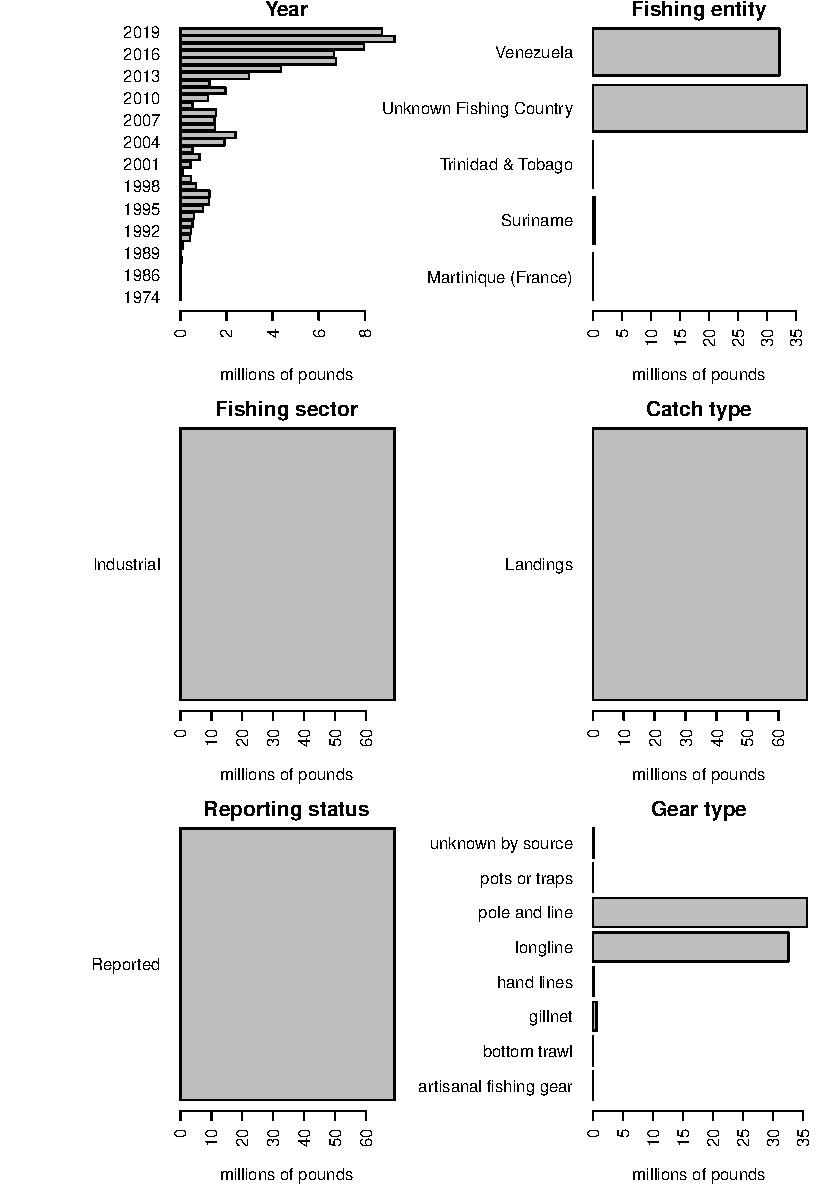
\includegraphics{SAU_EEZs_files/figure-pdf/unnamed-chunk-7-1.pdf}

Note that a large portion of the catch in the database is listed as
coming from an ``Unknown Fishing Country.'' We extract these catches and
further investigate the characteristics.

\begin{Shaded}
\begin{Highlighting}[]
\CommentTok{\# extract the Unknown Fishing Country catch}
\NormalTok{v1 }\OtherTok{\textless{}{-}}\NormalTok{ v[}\FunctionTok{which}\NormalTok{(v}\SpecialCharTok{$}\NormalTok{fishing\_entity }\SpecialCharTok{==} \StringTok{"Unknown Fishing Country"}\NormalTok{), ]}
\CommentTok{\#apply(v1[1:15], 2, table)}

\CommentTok{\# look at characteristics}
\FunctionTok{par}\NormalTok{(}\AttributeTok{mar =} \FunctionTok{c}\NormalTok{(}\DecValTok{3}\NormalTok{, }\DecValTok{10}\NormalTok{, }\DecValTok{1}\NormalTok{, }\DecValTok{5}\NormalTok{), }\AttributeTok{mfrow =} \FunctionTok{c}\NormalTok{(}\DecValTok{2}\NormalTok{, }\DecValTok{2}\NormalTok{), }\AttributeTok{mex =} \FloatTok{0.6}\NormalTok{)}
\FunctionTok{barplot}\NormalTok{(}\FunctionTok{tapply}\NormalTok{(v1}\SpecialCharTok{$}\NormalTok{pounds}\SpecialCharTok{/}\DecValTok{10}\SpecialCharTok{\^{}}\DecValTok{6}\NormalTok{, v1}\SpecialCharTok{$}\NormalTok{year, sum, }\AttributeTok{na.rm =}\NormalTok{ T), }\AttributeTok{las =} \DecValTok{2}\NormalTok{, }\AttributeTok{xlab =} \StringTok{"millions of pounds"}\NormalTok{, }\AttributeTok{main =} \StringTok{"Year"}\NormalTok{, }\AttributeTok{horiz =}\NormalTok{ T)}
\FunctionTok{barplot}\NormalTok{(}\FunctionTok{tapply}\NormalTok{(v1}\SpecialCharTok{$}\NormalTok{pounds}\SpecialCharTok{/}\DecValTok{10}\SpecialCharTok{\^{}}\DecValTok{6}\NormalTok{, v1}\SpecialCharTok{$}\NormalTok{fishing\_entity, sum, }\AttributeTok{na.rm =}\NormalTok{ T), }\AttributeTok{las =} \DecValTok{2}\NormalTok{, }\AttributeTok{xlab =} \StringTok{"millions of pounds"}\NormalTok{, }\AttributeTok{main =} \StringTok{"Fishing entity"}\NormalTok{, }\AttributeTok{horiz =}\NormalTok{ T)}
\FunctionTok{barplot}\NormalTok{(}\FunctionTok{tapply}\NormalTok{(v1}\SpecialCharTok{$}\NormalTok{pounds}\SpecialCharTok{/}\DecValTok{10}\SpecialCharTok{\^{}}\DecValTok{6}\NormalTok{, v1}\SpecialCharTok{$}\NormalTok{reporting\_status, sum, }\AttributeTok{na.rm =}\NormalTok{ T), }\AttributeTok{las =} \DecValTok{2}\NormalTok{, }\AttributeTok{xlab =} \StringTok{"millions of pounds"}\NormalTok{, }\AttributeTok{main =} \StringTok{"Reporting status"}\NormalTok{, }\AttributeTok{horiz =}\NormalTok{ T)}
\FunctionTok{barplot}\NormalTok{(}\FunctionTok{tapply}\NormalTok{(v1}\SpecialCharTok{$}\NormalTok{pounds}\SpecialCharTok{/}\DecValTok{10}\SpecialCharTok{\^{}}\DecValTok{6}\NormalTok{, v1}\SpecialCharTok{$}\NormalTok{gear\_type, sum, }\AttributeTok{na.rm =}\NormalTok{ T), }\AttributeTok{las =} \DecValTok{2}\NormalTok{, }\AttributeTok{xlab =} \StringTok{"millions of pounds"}\NormalTok{, }\AttributeTok{main =} \StringTok{"Gear type"}\NormalTok{, }\AttributeTok{horiz =}\NormalTok{ T)}
\end{Highlighting}
\end{Shaded}

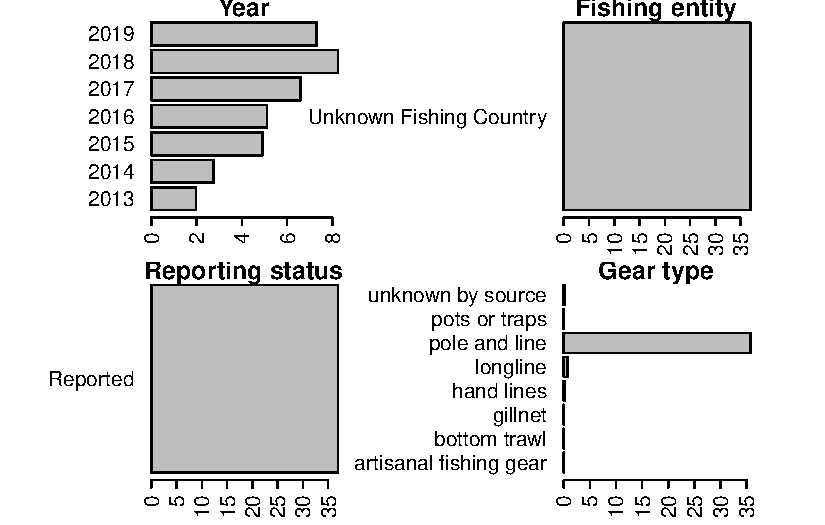
\includegraphics{SAU_EEZs_files/figure-pdf/unnamed-chunk-8-1.pdf}

Here is another look at the catches within the venezuelan EEZ, separated
by fishing entity.

\begin{Shaded}
\begin{Highlighting}[]
\CommentTok{\# summarize Venezuela EEZ catches by fishing entity}
\NormalTok{tab }\OtherTok{\textless{}{-}} \FunctionTok{tapply}\NormalTok{(v}\SpecialCharTok{$}\NormalTok{pounds, }\FunctionTok{list}\NormalTok{(v}\SpecialCharTok{$}\NormalTok{year, v}\SpecialCharTok{$}\NormalTok{fishing\_entity), sum, }\AttributeTok{na.rm =}\NormalTok{ T)}
\FunctionTok{head}\NormalTok{(tab)}
\end{Highlighting}
\end{Shaded}

\begin{verbatim}
     Martinique (France) Suriname Trinidad & Tobago Unknown Fishing Country
1974            7320.429       NA                NA                      NA
1976           12814.641       NA                NA                      NA
1985                  NA       NA                NA                      NA
1986                  NA       NA                NA                      NA
1987                  NA       NA                NA                      NA
1988                  NA       NA                NA                      NA
     Venezuela
1974        NA
1976        NA
1985  4699.563
1986  2229.484
1987  4585.610
1988 39960.149
\end{verbatim}

\begin{Shaded}
\begin{Highlighting}[]
\FunctionTok{matplot}\NormalTok{(}\FunctionTok{rownames}\NormalTok{(tab), tab}\SpecialCharTok{/}\DecValTok{10}\SpecialCharTok{\^{}}\DecValTok{6}\NormalTok{, }\AttributeTok{las =} \DecValTok{2}\NormalTok{, }\AttributeTok{type =} \StringTok{"b"}\NormalTok{, }\AttributeTok{lty =} \DecValTok{1}\NormalTok{, }\AttributeTok{lwd =} \DecValTok{2}\NormalTok{, }\AttributeTok{pch =} \DecValTok{19}\NormalTok{, }\AttributeTok{col =} \DecValTok{1}\SpecialCharTok{:}\DecValTok{5}\NormalTok{,}
        \AttributeTok{xlab =} \StringTok{""}\NormalTok{, }\AttributeTok{ylab =} \StringTok{"total catch (millions of pounds)"}\NormalTok{, }\AttributeTok{axes =}\NormalTok{ F, }
        \AttributeTok{main =} \StringTok{"Total dolphinfish catches in the Venezuelan EEZ"}\NormalTok{)}
\FunctionTok{axis}\NormalTok{(}\DecValTok{1}\NormalTok{, }\AttributeTok{at =} \FunctionTok{seq}\NormalTok{(}\DecValTok{1950}\NormalTok{, }\DecValTok{2020}\NormalTok{, }\DecValTok{5}\NormalTok{)); }\FunctionTok{axis}\NormalTok{(}\DecValTok{2}\NormalTok{, }\AttributeTok{las =} \DecValTok{2}\NormalTok{); }\FunctionTok{box}\NormalTok{()}
\FunctionTok{legend}\NormalTok{(}\StringTok{"topleft"}\NormalTok{, }\FunctionTok{colnames}\NormalTok{(tab), }\AttributeTok{col =} \DecValTok{1}\SpecialCharTok{:}\DecValTok{5}\NormalTok{, }\AttributeTok{pch =} \DecValTok{19}\NormalTok{, }\AttributeTok{lty =} \DecValTok{1}\NormalTok{, }\AttributeTok{lwd =} \DecValTok{3}\NormalTok{, }\AttributeTok{bty =} \StringTok{"n"}\NormalTok{, }\AttributeTok{title =} \StringTok{"Fishing entity"}\NormalTok{)}

\FunctionTok{text}\NormalTok{(}\DecValTok{2004}\NormalTok{, }\DecValTok{6}\NormalTok{, }\AttributeTok{cex =} \FloatTok{0.8}\NormalTok{,}
     \StringTok{"These Unknown Fishing Country}\SpecialCharTok{\textbackslash{}n}\StringTok{catches appear in the database as an}\SpecialCharTok{\textbackslash{}n}\StringTok{industrial fleet using pole and line gear}\SpecialCharTok{\textbackslash{}n}\StringTok{and are all listed as reported data}\SpecialCharTok{\textbackslash{}n}\StringTok{(\textquotesingle{}Assigned Tuna RFMO catch\textquotesingle{})"}\NormalTok{)}
\end{Highlighting}
\end{Shaded}

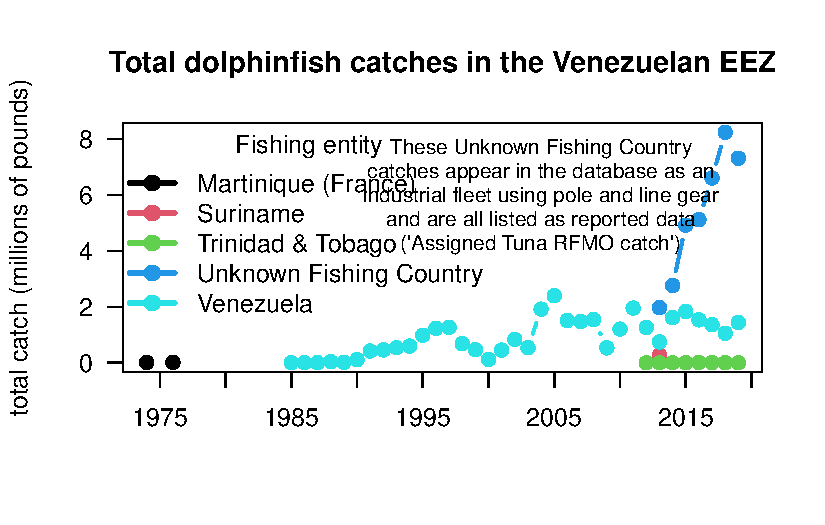
\includegraphics{SAU_EEZs_files/figure-pdf/unnamed-chunk-9-1.pdf}

The very substantial increase in international Western Atlantic dolphin
catches can be attributed solely to this Unknown Fishing Country catches
which appear in the database beginning in 2013. The documentation of the
catch reconstruction can be found in the Sea Around Us documentation
files (see Mendoza et al.~2015). We spoke to Jeremy Mendoza and other
experts who were involved in the reconstruction of domestic catches in
Venezuela, and they noted that the ``Assigned tuna RFMO catch'' actually
emerge from spatially reshuffled landing reports to ICCAT, according to
the methods of
\href{https://www.sciencedirect.com/science/article/abs/pii/S0165783619302346}{Coulter
et al.~(2020)}. In this work, the Sea Around Us team developed a global
spatial reallocation of landings of tunas and associated species that
were reported to ICCAT. In short, this work uses the fraction of
reported spatially disaggregated data to reallocate all data reported to
ICCAT. This step is necessary because there are not many countries that
report spatial data to ICCAT in the region, and this method may lead to
a significant reallocation of landings from the Caribbean to the
Venezuelan EEZ, where the local pole and line fishery is significant (J.
Mendoza, personal communication). Thus, it is likely that landings from
other EEZs, that were included in the reconstructed catch data layer,
could have been reassigned to the Venezuelan EEZ.

Because there may be some overlap between the reconstructed data used in
the national EEZ estimates, and the ICCAT reporting that was reassigned,
there could potentially be a ``double counting'' of these catch
estimates in the Sea Around Us database. We verified with Sea Around Us
database managers that their method led to an error resulting in an
overestimate of the catch, and they advised us to remove these Unknown
Fishing Country catches as they are difficult to trace back to the data
source.

\section{Compile catch in CAR and NED jurisdictional waters by discards
and reporting
type}\label{compile-catch-in-car-and-ned-jurisdictional-waters-by-discards-and-reporting-type}

Now that we have separated the EEZ catch by region, we will summarize it
according to the areas used in the dolphin management strategy
evaluation operating model. We will separate the catch by discards
versus landings and reported versus unreported data so that we can use
these data in various sensitivity analyses.

\begin{Shaded}
\begin{Highlighting}[]
\FunctionTok{rm}\NormalTok{(}\AttributeTok{list =} \FunctionTok{ls}\NormalTok{())  }\CommentTok{\# clear the workspace}

\CommentTok{\# load data}
\FunctionTok{load}\NormalTok{(}\StringTok{"data/outputs/SAU\_EEZs\_WCA.RData"}\NormalTok{)  }\CommentTok{\# SAU EEZ data for NED and NCA saved from earlier}
\FunctionTok{load}\NormalTok{(}\StringTok{"data/outputs/erroneous\_catch\_to\_be\_removed.RData"}\NormalTok{)   }\CommentTok{\# double{-}counted catch values to be removed}

\NormalTok{d }\OtherTok{\textless{}{-}}\NormalTok{ dwest}

\CommentTok{\# summarize the catch by area, discards/landings and reported/unreported}
\FunctionTok{tapply}\NormalTok{(d}\SpecialCharTok{$}\NormalTok{lbs, }\FunctionTok{list}\NormalTok{(d}\SpecialCharTok{$}\NormalTok{catch\_type, d}\SpecialCharTok{$}\NormalTok{reporting\_status, d}\SpecialCharTok{$}\NormalTok{reg), sum, }\AttributeTok{na.rm =}\NormalTok{ T)}
\end{Highlighting}
\end{Shaded}

\begin{verbatim}
, , Canadian EEZ

         Reported Unreported
Discards       NA         NA
Landings  1220146         NA

, , Western Central Atlantic EEZs

          Reported Unreported
Discards        NA    2179444
Landings 393279187  176215080
\end{verbatim}

The catch from the Canadian EEZs is 100\% landings, with no unreported
data and no discards. In the WCA there are no reported discards, only
unreported discards. Thus, we only need to separate out unreported
discards and landings for the WCA.

\begin{Shaded}
\begin{Highlighting}[]
\CommentTok{\# summarize the catch by year, area, discards/landings and reported/unreported}

\NormalTok{d}\SpecialCharTok{$}\NormalTok{year }\OtherTok{\textless{}{-}} \FunctionTok{factor}\NormalTok{(d}\SpecialCharTok{$}\NormalTok{year, }\AttributeTok{levels =} \DecValTok{1950}\SpecialCharTok{:}\DecValTok{2019}\NormalTok{)}
\NormalTok{dc }\OtherTok{\textless{}{-}}\NormalTok{ d[}\FunctionTok{which}\NormalTok{(d}\SpecialCharTok{$}\NormalTok{reg }\SpecialCharTok{==} \StringTok{"Canadian EEZ"}\NormalTok{), ]}
\NormalTok{dw }\OtherTok{\textless{}{-}}\NormalTok{ d[}\FunctionTok{which}\NormalTok{(d}\SpecialCharTok{$}\NormalTok{reg }\SpecialCharTok{==} \StringTok{"Western Central Atlantic EEZs"}\NormalTok{), ]}

\CommentTok{\# verify proper identification of the erroneous Venezuelan Unknown Fishing Country catches }
\NormalTok{bad }\OtherTok{\textless{}{-}}\NormalTok{ dw[}\FunctionTok{which}\NormalTok{(dw}\SpecialCharTok{$}\NormalTok{area\_name }\SpecialCharTok{==} \StringTok{"Venezuela"} \SpecialCharTok{\&}\NormalTok{ dw}\SpecialCharTok{$}\NormalTok{fishing\_entity }\SpecialCharTok{==} \StringTok{"Unknown Fishing Country"}\NormalTok{), ]}
\CommentTok{\#dim(bad)}
\NormalTok{bad\_totals }\OtherTok{\textless{}{-}} \FunctionTok{tapply}\NormalTok{(bad}\SpecialCharTok{$}\NormalTok{lbs, bad}\SpecialCharTok{$}\NormalTok{year, sum, }\AttributeTok{na.rm =}\NormalTok{ T)}

\FunctionTok{cbind}\NormalTok{(}\FunctionTok{tail}\NormalTok{(bad\_totals, }\DecValTok{10}\NormalTok{), }\FunctionTok{tail}\NormalTok{(removecatch, }\DecValTok{10}\NormalTok{)) }\CommentTok{\# the numbers match exactly}
\end{Highlighting}
\end{Shaded}

\begin{verbatim}
        [,1]    [,2]
2010      NA      NA
2011      NA      NA
2012      NA      NA
2013 1968566 1968566
2014 2759603 2759603
2015 4915156 4915156
2016 5112450 5112450
2017 6599737 6599737
2018 8236857 8236857
2019 7307245 7307245
\end{verbatim}

\begin{Shaded}
\begin{Highlighting}[]
\CommentTok{\# now remove those bad catches from the database prior to summarizing}
\CommentTok{\#dim(dw)}
\NormalTok{dw }\OtherTok{\textless{}{-}}\NormalTok{ dw[}\SpecialCharTok{{-}}\FunctionTok{which}\NormalTok{(dw}\SpecialCharTok{$}\NormalTok{area\_name }\SpecialCharTok{==} \StringTok{"Venezuela"} \SpecialCharTok{\&}\NormalTok{ dw}\SpecialCharTok{$}\NormalTok{fishing\_entity }\SpecialCharTok{==} \StringTok{"Unknown Fishing Country"}\NormalTok{), ]}
\CommentTok{\#dim(dw)}

\NormalTok{CAN }\OtherTok{\textless{}{-}} \FunctionTok{tapply}\NormalTok{(dc}\SpecialCharTok{$}\NormalTok{lbs, }\FunctionTok{list}\NormalTok{(dc}\SpecialCharTok{$}\NormalTok{year, dc}\SpecialCharTok{$}\NormalTok{catch\_type, dc}\SpecialCharTok{$}\NormalTok{reporting\_status), sum, }\AttributeTok{na.rm =}\NormalTok{ T)}
\FunctionTok{tail}\NormalTok{(CAN)}
\end{Highlighting}
\end{Shaded}

\begin{verbatim}
, , Reported

      Landings
2014 531022.55
2015  38945.76
2016 354370.65
2017  83776.88
2018  12588.88
2019  36112.19
\end{verbatim}

\begin{Shaded}
\begin{Highlighting}[]
\NormalTok{tab\_dw }\OtherTok{\textless{}{-}} \FunctionTok{tapply}\NormalTok{(dw}\SpecialCharTok{$}\NormalTok{lbs, }\FunctionTok{list}\NormalTok{(dw}\SpecialCharTok{$}\NormalTok{year, dw}\SpecialCharTok{$}\NormalTok{catch\_type, dw}\SpecialCharTok{$}\NormalTok{reporting\_status), sum, }\AttributeTok{na.rm =}\NormalTok{ T)}
\FunctionTok{tail}\NormalTok{(tab\_dw)}
\end{Highlighting}
\end{Shaded}

\begin{verbatim}
, , Reported

     Discards Landings
2014       NA  9923818
2015       NA 11590469
2016       NA 11225710
2017       NA 11702729
2018       NA 11460758
2019       NA 11066090

, , Unreported

     Discards Landings
2014 38062.63  2816498
2015 39134.61  2794662
2016 38973.17  2778493
2017 38728.81  2762926
2018 38769.93  2732351
2019 38655.51  2743182
\end{verbatim}

\begin{Shaded}
\begin{Highlighting}[]
\CommentTok{\# combine CAR reported landings, unreported discards, unreported landings}
\NormalTok{CAR }\OtherTok{\textless{}{-}} \FunctionTok{data.frame}\NormalTok{(}\FunctionTok{cbind}\NormalTok{(tab\_dw[, }\DecValTok{2}\NormalTok{, }\DecValTok{1}\NormalTok{], tab\_dw[, , }\DecValTok{2}\NormalTok{]))  }
\FunctionTok{names}\NormalTok{(CAR) }\OtherTok{\textless{}{-}} \FunctionTok{c}\NormalTok{(}\StringTok{"landings"}\NormalTok{, }\StringTok{"discards"}\NormalTok{, }\StringTok{"unreported"}\NormalTok{)}

\FunctionTok{matplot}\NormalTok{(}\FunctionTok{rownames}\NormalTok{(CAR), }\FunctionTok{cbind}\NormalTok{(CAN, CAR)}\SpecialCharTok{/}\DecValTok{10}\SpecialCharTok{\^{}}\DecValTok{6}\NormalTok{, }\AttributeTok{type =} \StringTok{"l"}\NormalTok{, }\AttributeTok{lwd =} \DecValTok{2}\NormalTok{, }\AttributeTok{lty =} \DecValTok{1}\NormalTok{, }\AttributeTok{col =} \DecValTok{2}\SpecialCharTok{:}\DecValTok{5}\NormalTok{,}
        \AttributeTok{xlab =} \StringTok{""}\NormalTok{, }\AttributeTok{ylab =} \StringTok{"total catch (millions of pounds)"}\NormalTok{,}
        \AttributeTok{main =} \StringTok{"Total dolphinfish catches in NED and NCA jurisdictional waters"}\NormalTok{)}
\FunctionTok{legend}\NormalTok{(}\StringTok{"topleft"}\NormalTok{, }\AttributeTok{col =} \DecValTok{2}\SpecialCharTok{:}\DecValTok{5}\NormalTok{, }\FunctionTok{c}\NormalTok{(}\StringTok{"Canadian reported landings"}\NormalTok{, }\StringTok{"Caribbean landings"}\NormalTok{, }
                    \StringTok{"Caribbean discards"}\NormalTok{, }\StringTok{"Caribbean unreported landings"}\NormalTok{), }\AttributeTok{lty =} \DecValTok{1}\NormalTok{, }\AttributeTok{lwd =} \DecValTok{3}\NormalTok{, }\AttributeTok{bty =} \StringTok{"n"}\NormalTok{)}
\end{Highlighting}
\end{Shaded}

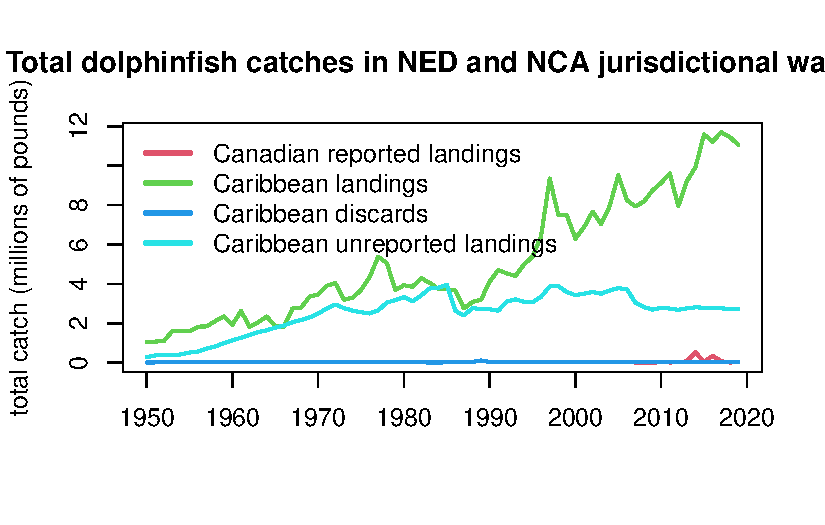
\includegraphics{SAU_EEZs_files/figure-pdf/unnamed-chunk-12-1.pdf}

\begin{Shaded}
\begin{Highlighting}[]
\FunctionTok{round}\NormalTok{(}\FunctionTok{sum}\NormalTok{(CAR}\SpecialCharTok{$}\NormalTok{discards, }\AttributeTok{na.rm =}\NormalTok{ T) }\SpecialCharTok{/}\NormalTok{ (}\FunctionTok{sum}\NormalTok{(CAR}\SpecialCharTok{$}\NormalTok{discards, }\AttributeTok{na.rm =}\NormalTok{ T) }\SpecialCharTok{+} \FunctionTok{sum}\NormalTok{(CAR}\SpecialCharTok{$}\NormalTok{landings, }\AttributeTok{na.rm =}\NormalTok{ T)) }\SpecialCharTok{*} \DecValTok{100}\NormalTok{, }\DecValTok{2}\NormalTok{)  }\CommentTok{\# discards are 0.6\% of landings}
\end{Highlighting}
\end{Shaded}

\begin{verbatim}
[1] 0.61
\end{verbatim}

Note that the Caribbean unreported discards in the database are
negligible (\textless{} 1\%) and we exclude them from further analysis.

\section{Distribute the territorial international catches across
quarters of the
year}\label{distribute-the-territorial-international-catches-across-quarters-of-the-year}

The international landings are only reported as annual catches and do
not have any month or season associated with them. However, the MSE
operating model requires seasonal catches. Lacking other information on
the seasonality of these fleets, we will assume that the fleet
distribution of the U.S. pelagic longline is representative of the
seasonality of the jurisdictional fleets. Now we parse the annual
catches according to the seasonality of the U.S. fleet.

The pelagic longline logbook data is only available going back to 1997,
but there are Caribbean catches extending back to the 1950s. To
interpolate the seasonality for 1986 - 1996, we take the average
seasonality of the oldest 10 years of logbook data (1997 - 2006) and use
those averages for the unknown years.

At the time of analysis, the SAU database only contained catches to
2019, so we interpolated the 2019 values to cover years 2020 - 2022.

\begin{Shaded}
\begin{Highlighting}[]
\CommentTok{\#par(mar = c(5, 10, 3, 1))}
\CommentTok{\#barplot(tapply(dw$lbs, dw$gear\_type, sum, na.rm = T), horiz = T, las = 2)}
\CommentTok{\#barplot(tapply(dc$lbs, dc$gear\_type, sum, na.rm = T), horiz = T, las = 2)}

\CommentTok{\# read in the percentage of the catch by area and year{-}quarter combinations from the U.S. PLL}
\FunctionTok{load}\NormalTok{(}\StringTok{"data/outputs/per\_PLLcatch\_by\_area\_yearquarter.RData"}\NormalTok{)  }

\FunctionTok{names}\NormalTok{(percatch[}\DecValTok{1}\NormalTok{, }\DecValTok{1}\NormalTok{, ]) }\CommentTok{\# matrix 2 == Caribbean, matrix 7 == NED (Atlantic Northwest)}
\end{Highlighting}
\end{Shaded}

\begin{verbatim}
[1] "NCA"  "CAR"  "FLK"  "NCFL" "NNC"  "VBM"  "NED" 
\end{verbatim}

\begin{Shaded}
\begin{Highlighting}[]
\NormalTok{CAN }\OtherTok{\textless{}{-}}\NormalTok{ CAN[}\FunctionTok{which}\NormalTok{(}\FunctionTok{rownames}\NormalTok{(CAN) }\SpecialCharTok{\textgreater{}=} \DecValTok{1997}\NormalTok{)]  }\CommentTok{\# PLL data are only available from 1997 on }
\NormalTok{CAN }\OtherTok{\textless{}{-}} \FunctionTok{c}\NormalTok{(CAN, CAN[}\FunctionTok{length}\NormalTok{(CAN)], CAN[}\FunctionTok{length}\NormalTok{(CAN)], CAN[}\FunctionTok{length}\NormalTok{(CAN)])  }\CommentTok{\# interpolate 2019 catches for 2020{-}2022}

\NormalTok{CANqrt }\OtherTok{\textless{}{-}}\NormalTok{ percatch[, , }\DecValTok{7}\NormalTok{]   }\CommentTok{\# create matrix for final catch data}
\ControlFlowTok{for}\NormalTok{ (i }\ControlFlowTok{in} \DecValTok{1}\SpecialCharTok{:}\FunctionTok{ncol}\NormalTok{(percatch))  \{ }
\NormalTok{  CANqrt[, i] }\OtherTok{\textless{}{-}}\NormalTok{ percatch[, i, }\DecValTok{7}\NormalTok{] }\SpecialCharTok{*}\NormalTok{ CAN[i]  \}}

\NormalTok{percatch\_car }\OtherTok{\textless{}{-}}\NormalTok{ percatch[, , }\DecValTok{2}\NormalTok{] }\CommentTok{\# create matrix for Caribbean percentages}
\NormalTok{int }\OtherTok{\textless{}{-}} \FunctionTok{rowMeans}\NormalTok{(percatch\_car[, }\DecValTok{1}\SpecialCharTok{:}\DecValTok{10}\NormalTok{]) }\CommentTok{\# calculate the average seasonality using the oldest 10 years of logbook data}
\NormalTok{percatch\_car }\OtherTok{\textless{}{-}} \FunctionTok{cbind}\NormalTok{(}\FunctionTok{matrix}\NormalTok{(}\FunctionTok{rep}\NormalTok{(int, }\FunctionTok{length}\NormalTok{(}\DecValTok{1986}\SpecialCharTok{:}\DecValTok{1996}\NormalTok{)), }\AttributeTok{nrow =} \DecValTok{4}\NormalTok{), percatch\_car)  }\CommentTok{\# attach those 10{-}year averages to years 1986:1996}
\FunctionTok{colnames}\NormalTok{(percatch\_car) }\OtherTok{\textless{}{-}} \DecValTok{1986}\SpecialCharTok{:}\DecValTok{2022}   \CommentTok{\# full data frame for Caribbean seasonality 1986 {-} 2022}

\NormalTok{CAR }\OtherTok{\textless{}{-}}\NormalTok{ CAR[}\FunctionTok{which}\NormalTok{(}\FunctionTok{rownames}\NormalTok{(CAR) }\SpecialCharTok{\textgreater{}=} \DecValTok{1986}\NormalTok{), ]  }\CommentTok{\# only need Caribbean data from 1986 on }
\NormalTok{CAR }\OtherTok{\textless{}{-}} \FunctionTok{rbind}\NormalTok{(CAR, CAR[}\FunctionTok{nrow}\NormalTok{(CAR), ], CAR[}\FunctionTok{nrow}\NormalTok{(CAR), ], CAR[}\FunctionTok{nrow}\NormalTok{(CAR), ])  }\CommentTok{\# interpolate 2019 catches for 2020{-}2022}

\CommentTok{\#dim(CAR)}
\CommentTok{\#dim(percatch\_car)}

\NormalTok{CARrep }\OtherTok{\textless{}{-}}\NormalTok{ percatch\_car   }\CommentTok{\# create matrices for final catch data}
\NormalTok{CARunr }\OtherTok{\textless{}{-}}\NormalTok{ percatch\_car}

\ControlFlowTok{for}\NormalTok{ (i }\ControlFlowTok{in} \DecValTok{1}\SpecialCharTok{:}\FunctionTok{ncol}\NormalTok{(percatch\_car))  \{ }
\NormalTok{  CARrep[, i] }\OtherTok{\textless{}{-}}\NormalTok{ percatch\_car[, i] }\SpecialCharTok{*}\NormalTok{ CAR[i, }\DecValTok{1}\NormalTok{]}
\NormalTok{  CARunr[, i] }\OtherTok{\textless{}{-}}\NormalTok{ percatch\_car[, i] }\SpecialCharTok{*}\NormalTok{ CAR[i, }\DecValTok{3}\NormalTok{]}
\NormalTok{\}}

\CommentTok{\# ensure sums are equal after parsing}
\FunctionTok{sum}\NormalTok{(CARrep); }\FunctionTok{sum}\NormalTok{(CAR}\SpecialCharTok{$}\NormalTok{landings)}
\end{Highlighting}
\end{Shaded}

\begin{verbatim}
[1] 286220280
\end{verbatim}

\begin{verbatim}
[1] 286220280
\end{verbatim}

\begin{Shaded}
\begin{Highlighting}[]
\FunctionTok{sum}\NormalTok{(CARunr); }\FunctionTok{sum}\NormalTok{(CAR}\SpecialCharTok{$}\NormalTok{unreported)}
\end{Highlighting}
\end{Shaded}

\begin{verbatim}
[1] 112754888
\end{verbatim}

\begin{verbatim}
[1] 112754888
\end{verbatim}

\begin{Shaded}
\begin{Highlighting}[]
\FunctionTok{sum}\NormalTok{(CAN, }\AttributeTok{na.rm =}\NormalTok{ T); }\FunctionTok{sum}\NormalTok{(CANqrt, }\AttributeTok{na.rm =}\NormalTok{ T)}
\end{Highlighting}
\end{Shaded}

\begin{verbatim}
[1] 1328482
\end{verbatim}

\begin{verbatim}
[1] 1328482
\end{verbatim}

The Canada jurisdictional data need to be combined with the NED high
seas data calculated in the previous section, because both of these are
a component of the international catches in the NED area.

\begin{Shaded}
\begin{Highlighting}[]
\FunctionTok{load}\NormalTok{(}\StringTok{"data/outputs/NED\_year\_quarter.RData"}\NormalTok{)}

\NormalTok{NEDtot }\OtherTok{\textless{}{-}}\NormalTok{ NED }\SpecialCharTok{+}\NormalTok{ CANqrt}
\CommentTok{\# ensure sums are correct}
\FunctionTok{sum}\NormalTok{(NED, }\AttributeTok{na.rm =}\NormalTok{ T) }\SpecialCharTok{+} \FunctionTok{sum}\NormalTok{(CANqrt, }\AttributeTok{na.rm =}\NormalTok{ T); }\FunctionTok{sum}\NormalTok{(NEDtot, }\AttributeTok{na.rm =}\NormalTok{ T)}
\end{Highlighting}
\end{Shaded}

\begin{verbatim}
[1] 1808855
\end{verbatim}

\begin{verbatim}
[1] 1808855
\end{verbatim}

\begin{Shaded}
\begin{Highlighting}[]
\NormalTok{NEDtot }\OtherTok{\textless{}{-}}\NormalTok{ NEDtot[, }\SpecialCharTok{!}\FunctionTok{is.na}\NormalTok{(}\FunctionTok{colSums}\NormalTok{(NEDtot))] }\CommentTok{\# remove NA columns from CAN data}

\CommentTok{\# plot the parsed out data by year{-}quarter}
\NormalTok{yrs }\OtherTok{\textless{}{-}} \FunctionTok{sort}\NormalTok{(}\FunctionTok{rep}\NormalTok{(}\FunctionTok{as.numeric}\NormalTok{(}\FunctionTok{colnames}\NormalTok{(CARrep)), }\DecValTok{4}\NormalTok{))}
\NormalTok{qrt }\OtherTok{\textless{}{-}} \FunctionTok{rep}\NormalTok{(}\DecValTok{1}\SpecialCharTok{:}\DecValTok{4}\NormalTok{, }\FunctionTok{length}\NormalTok{(yrs)}\SpecialCharTok{/}\DecValTok{4}\NormalTok{)}
\NormalTok{yrs1 }\OtherTok{\textless{}{-}} \FunctionTok{sort}\NormalTok{(}\FunctionTok{rep}\NormalTok{(}\FunctionTok{as.numeric}\NormalTok{(}\FunctionTok{colnames}\NormalTok{(NEDtot)), }\DecValTok{4}\NormalTok{))}
\NormalTok{qrt1 }\OtherTok{\textless{}{-}} \FunctionTok{rep}\NormalTok{(}\DecValTok{1}\SpecialCharTok{:}\DecValTok{4}\NormalTok{, }\FunctionTok{length}\NormalTok{(yrs1)}\SpecialCharTok{/}\DecValTok{4}\NormalTok{)}

\FunctionTok{matplot}\NormalTok{(yrs }\SpecialCharTok{+}\NormalTok{ qrt}\SpecialCharTok{/}\DecValTok{4}\NormalTok{, }\FunctionTok{cbind}\NormalTok{(}\FunctionTok{matrix}\NormalTok{(CARrep), }\FunctionTok{matrix}\NormalTok{(CARunr))}\SpecialCharTok{/}\DecValTok{10}\SpecialCharTok{\^{}}\DecValTok{6}\NormalTok{, }\AttributeTok{lty =} \DecValTok{1}\NormalTok{, }\AttributeTok{lwd =} \DecValTok{2}\NormalTok{, }
        \AttributeTok{col =} \DecValTok{2}\SpecialCharTok{:}\DecValTok{3}\NormalTok{, }\AttributeTok{type =} \StringTok{"l"}\NormalTok{, }\AttributeTok{main =} \StringTok{"International jurisdictional catches by quarter"}\NormalTok{, }
        \AttributeTok{xlab =} \StringTok{""}\NormalTok{, }\AttributeTok{ylab =} \StringTok{"total catch (millions of pounds)"}\NormalTok{)}
\FunctionTok{lines}\NormalTok{(yrs1 }\SpecialCharTok{+}\NormalTok{ qrt1}\SpecialCharTok{/}\DecValTok{4}\NormalTok{, }\FunctionTok{as.numeric}\NormalTok{(}\FunctionTok{matrix}\NormalTok{(NEDtot))}\SpecialCharTok{/}\DecValTok{10}\SpecialCharTok{\^{}}\DecValTok{6}\NormalTok{, }\AttributeTok{lwd =} \DecValTok{2}\NormalTok{, }\AttributeTok{col =} \DecValTok{4}\NormalTok{)}
\FunctionTok{legend}\NormalTok{(}\StringTok{"topleft"}\NormalTok{, }\FunctionTok{c}\NormalTok{(}\StringTok{"Caribbean reported landings"}\NormalTok{, }\StringTok{"Caribbean unreported landings"}\NormalTok{, }\StringTok{"NED reported landings"}\NormalTok{),        }
       \AttributeTok{lwd =} \DecValTok{2}\NormalTok{, }\AttributeTok{col =} \DecValTok{2}\SpecialCharTok{:}\DecValTok{4}\NormalTok{, }\AttributeTok{bty =} \StringTok{"n"}\NormalTok{)}
\end{Highlighting}
\end{Shaded}

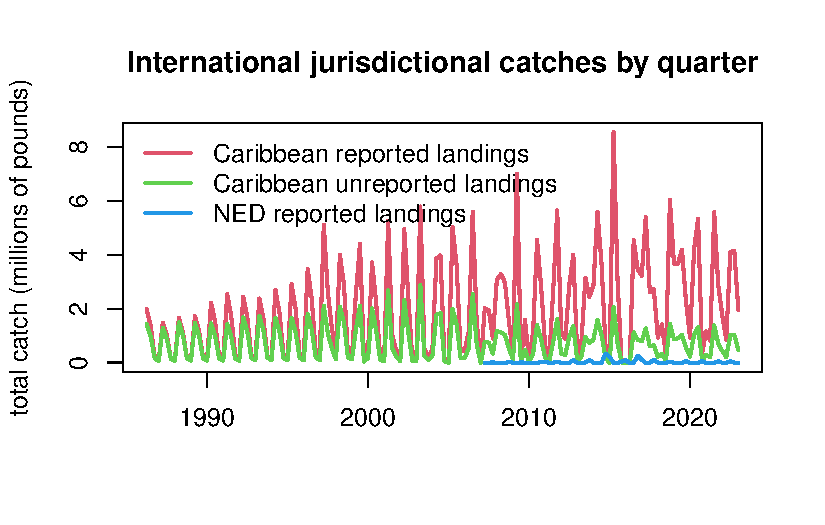
\includegraphics{SAU_EEZs_files/figure-pdf/unnamed-chunk-14-1.pdf}

Finally, we format the data in the format for input into the operating
model.

\begin{Shaded}
\begin{Highlighting}[]
\CommentTok{\# format for operating model {-} Caribbean }
\NormalTok{flt }\OtherTok{\textless{}{-}} \FunctionTok{rep}\NormalTok{(}\StringTok{"Intl"}\NormalTok{, }\FunctionTok{length}\NormalTok{(yrs))}
\NormalTok{are }\OtherTok{\textless{}{-}} \FunctionTok{rep}\NormalTok{(}\StringTok{"CAR"}\NormalTok{, }\FunctionTok{length}\NormalTok{(yrs))}
\NormalTok{fin1 }\OtherTok{\textless{}{-}} \FunctionTok{data.frame}\NormalTok{(}\FunctionTok{cbind}\NormalTok{(yrs, qrt, flt, are, }\FunctionTok{matrix}\NormalTok{(CARrep)))}
\NormalTok{flt }\OtherTok{\textless{}{-}} \FunctionTok{rep}\NormalTok{(}\StringTok{"UnRep"}\NormalTok{, }\FunctionTok{length}\NormalTok{(yrs))}
\NormalTok{fin2 }\OtherTok{\textless{}{-}} \FunctionTok{data.frame}\NormalTok{(}\FunctionTok{cbind}\NormalTok{(yrs, qrt, flt, are, }\FunctionTok{matrix}\NormalTok{(CARunr)))}

\NormalTok{findat }\OtherTok{\textless{}{-}} \FunctionTok{data.frame}\NormalTok{(}\FunctionTok{rbind}\NormalTok{(fin1, fin2), }\AttributeTok{stringsAsFactors =} \ConstantTok{FALSE}\NormalTok{)}
\FunctionTok{names}\NormalTok{(findat) }\OtherTok{\textless{}{-}} \FunctionTok{c}\NormalTok{(}\StringTok{"Year"}\NormalTok{, }\StringTok{"Quarter"}\NormalTok{, }\StringTok{"Fleet"}\NormalTok{, }\StringTok{"Area"}\NormalTok{, }\StringTok{"Catch\_lbs"}\NormalTok{)}
\NormalTok{findat}\SpecialCharTok{$}\NormalTok{Catch\_lbs }\OtherTok{\textless{}{-}} \FunctionTok{as.numeric}\NormalTok{(findat}\SpecialCharTok{$}\NormalTok{Catch\_lbs)}
\FunctionTok{head}\NormalTok{(findat)}
\end{Highlighting}
\end{Shaded}

\begin{verbatim}
  Year Quarter Fleet Area Catch_lbs
1 1986       1  Intl  CAR 1983610.3
2 1986       2  Intl  CAR 1363432.3
3 1986       3  Intl  CAR  216194.7
4 1986       4  Intl  CAR  104564.4
5 1987       1  Intl  CAR 1491251.1
6 1987       2  Intl  CAR 1025009.7
\end{verbatim}

\begin{Shaded}
\begin{Highlighting}[]
\CommentTok{\#plot(findat$Catch\_lbs, type = "l")}
\CommentTok{\#plot(findat$Catch\_lbs \textasciitilde{} factor(findat$Fleet))}
\CommentTok{\#plot(findat$Catch\_lbs \textasciitilde{} factor(findat$Quarter))}
\CommentTok{\#plot(findat$Catch\_lbs \textasciitilde{} factor(findat$Year))}
\CommentTok{\#apply(findat, 2, table)}

\CommentTok{\# write the output file}
\FunctionTok{write.csv}\NormalTok{(findat, }\AttributeTok{file =} \StringTok{"data/FINAL\_files/CAR\_Intl\_unrep\_TomFormat.csv"}\NormalTok{, }\AttributeTok{row.names =} \ConstantTok{FALSE}\NormalTok{)}

\CommentTok{\# format for operating model {-} NED }
\NormalTok{flt }\OtherTok{\textless{}{-}} \FunctionTok{rep}\NormalTok{(}\StringTok{"Intl"}\NormalTok{, }\FunctionTok{length}\NormalTok{(yrs1))}
\NormalTok{are }\OtherTok{\textless{}{-}} \FunctionTok{rep}\NormalTok{(}\StringTok{"NED"}\NormalTok{, }\FunctionTok{length}\NormalTok{(yrs1))}
\NormalTok{fin }\OtherTok{\textless{}{-}} \FunctionTok{data.frame}\NormalTok{(}\FunctionTok{cbind}\NormalTok{(yrs1, qrt1, flt, are, }\FunctionTok{matrix}\NormalTok{(NEDtot)), }\AttributeTok{stringsAsFactors =} \ConstantTok{FALSE}\NormalTok{)}
\FunctionTok{names}\NormalTok{(fin) }\OtherTok{\textless{}{-}} \FunctionTok{c}\NormalTok{(}\StringTok{"Year"}\NormalTok{, }\StringTok{"Quarter"}\NormalTok{, }\StringTok{"Fleet"}\NormalTok{, }\StringTok{"Area"}\NormalTok{, }\StringTok{"Catch\_lbs"}\NormalTok{)}
\NormalTok{fin}\SpecialCharTok{$}\NormalTok{Catch\_lbs }\OtherTok{\textless{}{-}} \FunctionTok{as.numeric}\NormalTok{(fin}\SpecialCharTok{$}\NormalTok{Catch\_lbs)}
\FunctionTok{head}\NormalTok{(fin)}
\end{Highlighting}
\end{Shaded}

\begin{verbatim}
  Year Quarter Fleet Area Catch_lbs
1 2007       1  Intl  NED     0.000
2 2007       2  Intl  NED  1450.366
3 2007       3  Intl  NED 13279.912
4 2007       4  Intl  NED     0.000
5 2008       1  Intl  NED     0.000
6 2008       2  Intl  NED  1312.750
\end{verbatim}

\begin{Shaded}
\begin{Highlighting}[]
\CommentTok{\#apply(fin, 2, table)}

\CommentTok{\# write output file}
\FunctionTok{write.csv}\NormalTok{(fin, }\AttributeTok{file =} \StringTok{"data/FINAL\_files/NED\_Intl\_TomFormat.csv"}\NormalTok{, }\AttributeTok{row.names =} \ConstantTok{FALSE}\NormalTok{)}

\CommentTok{\#barplot(tapply(fin$Catch\_lbs, list(fin$Quarter), sum, na.rm = T), col = rainbow(4))}
\end{Highlighting}
\end{Shaded}

\section{References}\label{references}

Pauly D., Zeller D., Palomares M.L.D. (Editors), 2020. Sea Around Us
Concepts, Design and Data (seaaroundus.org).

\bookmarksetup{startatroot}

\chapter{Data compilation for all fleets in the operating
model}\label{data-compilation-for-all-fleets-in-the-operating-model}

In this last step we will compile all of the output data files from the
different data sources (NMFS commercial trip tickets, NMFS recreational
statistics, Sea Around Us) and check the files for accuracy.

Recall that there are seven defined areas in the operating model, over
which the catches are summed. Four of these areas are within the U.S.
EEZ and the other three areas are international waters (high seas and
jurisdictional waters of other countries).

\begin{figure}[H]

{\centering 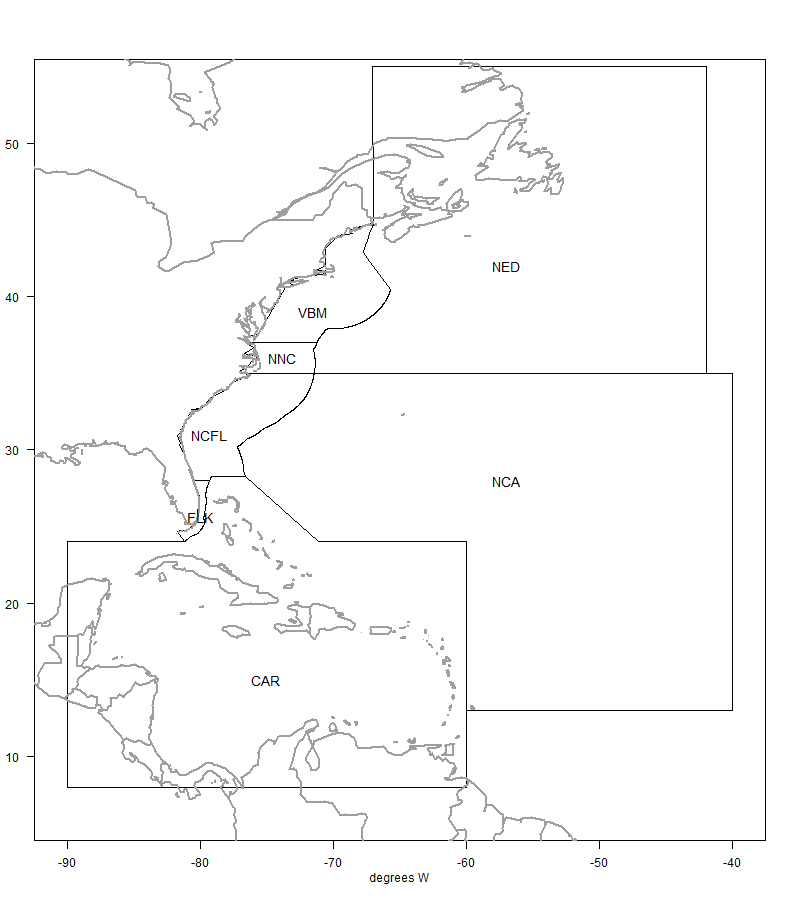
\includegraphics{data/eez/new_spatial_zones1.png}

}

\caption{Areas defined in the operating model.}

\end{figure}%

\section{Data upload}\label{data-upload}

First we access all of the final data files from the previous steps.

\begin{Shaded}
\begin{Highlighting}[]
\CommentTok{\# clear workspace}
\FunctionTok{rm}\NormalTok{(}\AttributeTok{list =} \FunctionTok{ls}\NormalTok{())}

\CommentTok{\# view data files in directory}
\FunctionTok{dir}\NormalTok{(}\StringTok{"data/FINAL\_files/"}\NormalTok{)}
\end{Highlighting}
\end{Shaded}

\begin{verbatim}
[1] "CAR_Intl_unrep_TomFormat.csv"        
[2] "commercial_TomFormat.csv"            
[3] "complete_catch_dataset_09052025b.csv"
[4] "NCA_Intl_TomFormat.csv"              
[5] "NED_Intl_TomFormat.csv"              
[6] "rec_catch_TomFormat.csv"             
\end{verbatim}

\begin{Shaded}
\begin{Highlighting}[]
\NormalTok{intc }\OtherTok{\textless{}{-}} \FunctionTok{read.csv}\NormalTok{(}\StringTok{"data/FINAL\_files/CAR\_Intl\_unrep\_TomFormat.csv"}\NormalTok{)}
\NormalTok{intn }\OtherTok{\textless{}{-}} \FunctionTok{read.csv}\NormalTok{(}\StringTok{"data/FINAL\_files/NCA\_Intl\_TomFormat.csv"}\NormalTok{)}
\NormalTok{intw }\OtherTok{\textless{}{-}} \FunctionTok{read.csv}\NormalTok{(}\StringTok{"data/FINAL\_files/NED\_Intl\_TomFormat.csv"}\NormalTok{)}
\NormalTok{com }\OtherTok{\textless{}{-}} \FunctionTok{read.csv}\NormalTok{(}\StringTok{"data/FINAL\_files/commercial\_TomFormat.csv"}\NormalTok{)}
\NormalTok{rec }\OtherTok{\textless{}{-}} \FunctionTok{read.csv}\NormalTok{(}\StringTok{"data/FINAL\_files/rec\_catch\_TomFormat.csv"}\NormalTok{)}
\end{Highlighting}
\end{Shaded}

This file contains all international catches and unreported catches for
the greater Caribbean region (jurisdictional waters of all countries).
Recall that estimated discards were very small (\textless{} 1\%) and
were removed from the summary.

\begin{verbatim}
$Year

1986 1987 1988 1989 1990 1991 1992 1993 1994 1995 1996 1997 1998 1999 2000 2001 
   8    8    8    8    8    8    8    8    8    8    8    8    8    8    8    8 
2002 2003 2004 2005 2006 2007 2008 2009 2010 2011 2012 2013 2014 2015 2016 2017 
   8    8    8    8    8    8    8    8    8    8    8    8    8    8    8    8 
2018 2019 2020 2021 2022 <NA> 
   8    8    8    8    8    0 

$Quarter

   1    2    3    4 <NA> 
  74   74   74   74    0 

$Fleet

 Intl UnRep  <NA> 
  148   148     0 

$Area

 CAR <NA> 
 296    0 
\end{verbatim}

This file contains all international catches for the NCA region (i.e.,
FAO region 31), also known as the Western Central Atlantic. There are no
territorial waters in this area (except for Bermuda, which as discussed
previously is summarized with the CAR region) and there are no
unreported catches or discards in the database.

\begin{verbatim}
$Year

1997 1998 1999 2000 2001 2002 2003 2004 2005 2006 2007 2008 2009 2010 2011 2012 
   4    4    4    4    4    4    4    4    4    4    4    4    4    4    4    4 
2013 2014 2015 2016 2017 2018 2019 2020 2021 2022 <NA> 
   4    4    4    4    4    4    4    4    4    4    0 

$Quarter

   1    2    3    4 <NA> 
  26   26   26   26    0 

$Fleet

Intl <NA> 
 104    0 

$Area

 NCA <NA> 
 104    0 
\end{verbatim}

This file contains all international catches for the NED region (i.e.,
FAO region 21), also known as the Northwest Atlantic. This includes NED
high seas catches, as well as catches from Canadian and French
territorial waters which fall in this region. There are no unreported
catches or discards for this region in the database.

\begin{verbatim}
$Year

2007 2008 2009 2010 2011 2012 2013 2014 2015 2016 2017 2018 2019 2020 2021 2022 
   4    4    4    4    4    4    4    4    4    4    4    4    4    4    4    4 
<NA> 
   0 

$Quarter

   1    2    3    4 <NA> 
  16   16   16   16    0 

$Fleet

Intl <NA> 
  64    0 

$Area

 NED <NA> 
  64    0 
\end{verbatim}

This file contains all catches for the U.S. commercial fleet, including
catches from U.S. EEZs and high seas. There are no unreported catches in
this region. Recall that estimated dead discards were very small
(\textless{} 2\%) and were removed from the summary.

\begin{verbatim}
$Year

1986 1987 1988 1989 1990 1991 1992 1993 1994 1995 1996 1997 1998 1999 2000 2001 
  28   28   28   28   28   28   28   28   28   28   28   28   28   28   28   28 
2002 2003 2004 2005 2006 2007 2008 2009 2010 2011 2012 2013 2014 2015 2016 2017 
  28   28   28   28   28   28   28   28   28   28   28   28   28   28   28   28 
2018 2019 2020 2021 2022 <NA> 
  28   28   28   28   28    0 

$Quarter

   1    2    3    4 <NA> 
 259  259  259  259    0 

$Fleet

UScom  <NA> 
 1036     0 

$Area

 CAR  FLK  NCA NCFL  NED  NNC  VBM <NA> 
 148  148  148  148  148  148  148    0 
\end{verbatim}

This file contains all catches for the U.S. recreational fleet, which
are all assumed to occur within the U.S. EEZs. There are no unreported
catches in this region.

\begin{verbatim}
$Year

1986 1987 1988 1989 1990 1991 1992 1993 1994 1995 1996 1997 1998 1999 2000 2001 
  32   32   32   32   32   32   32   32   32   32   32   32   32   32   32   32 
2002 2003 2004 2005 2006 2007 2008 2009 2010 2011 2012 2013 2014 2015 2016 2017 
  32   32   32   32   32   32   32   32   32   32   32   32   32   32   32   32 
2018 2019 2020 2021 2022 <NA> 
  32   32   32   32   32    0 

$Quarter

   1    2    3    4 <NA> 
 296  296  296  296    0 

$Fleet

Hire  Rec <NA> 
 592  592    0 

$Area

 FLK NCFL  NNC  VBM <NA> 
 296  296  296  296    0 
\end{verbatim}

Now we combine the data files and create some figures with the final
composite data file.

\begin{verbatim}

FALSE  TRUE 
 2047   637 
\end{verbatim}

\section{Visualizing the final data
set}\label{visualizing-the-final-data-set}

We plot the final data set in a number of different ways to detect any
errors that may have occurred during processing.

\begin{Shaded}
\begin{Highlighting}[]
\CommentTok{\# plot the total catches by each factor}
\FunctionTok{par}\NormalTok{(}\AttributeTok{mfrow =} \FunctionTok{c}\NormalTok{(}\DecValTok{2}\NormalTok{, }\DecValTok{2}\NormalTok{), }\AttributeTok{mex =} \FloatTok{0.7}\NormalTok{)}
\FunctionTok{barplot}\NormalTok{(}\FunctionTok{tapply}\NormalTok{(d}\SpecialCharTok{$}\NormalTok{Catch\_lbs, d}\SpecialCharTok{$}\NormalTok{Year, sum, }\AttributeTok{na.rm =}\NormalTok{ T)}\SpecialCharTok{/}\DecValTok{10}\SpecialCharTok{\^{}}\DecValTok{6}\NormalTok{, }\AttributeTok{las =} \DecValTok{2}\NormalTok{,}
        \AttributeTok{main =} \StringTok{"Total catch by year"}\NormalTok{, }\AttributeTok{ylab =} \StringTok{"total catch (millions of pounds)"}\NormalTok{)}
\FunctionTok{barplot}\NormalTok{(}\FunctionTok{tapply}\NormalTok{(d}\SpecialCharTok{$}\NormalTok{Catch\_lbs, d}\SpecialCharTok{$}\NormalTok{Quarter, sum, }\AttributeTok{na.rm =}\NormalTok{ T)}\SpecialCharTok{/}\DecValTok{10}\SpecialCharTok{\^{}}\DecValTok{6}\NormalTok{, }
        \AttributeTok{ylab =} \StringTok{"total catch (millions of pounds)"}\NormalTok{, }\AttributeTok{main =} \StringTok{"Total catch by quarter"}\NormalTok{)}
\FunctionTok{barplot}\NormalTok{(}\FunctionTok{tapply}\NormalTok{(d}\SpecialCharTok{$}\NormalTok{Catch\_lbs, d}\SpecialCharTok{$}\NormalTok{Fleet, sum, }\AttributeTok{na.rm =}\NormalTok{ T)}\SpecialCharTok{/}\DecValTok{10}\SpecialCharTok{\^{}}\DecValTok{6}\NormalTok{, }
        \AttributeTok{main =} \StringTok{"Total catch by fleet"}\NormalTok{, }\AttributeTok{ylab =} \StringTok{"total catch (millions of pounds)"}\NormalTok{)}
\FunctionTok{barplot}\NormalTok{(}\FunctionTok{tapply}\NormalTok{(d}\SpecialCharTok{$}\NormalTok{Catch\_lbs, d}\SpecialCharTok{$}\NormalTok{Area, sum, }\AttributeTok{na.rm =}\NormalTok{ T)}\SpecialCharTok{/}\DecValTok{10}\SpecialCharTok{\^{}}\DecValTok{6}\NormalTok{, }
        \AttributeTok{main =} \StringTok{"Total catch by area"}\NormalTok{, }\AttributeTok{ylab =} \StringTok{"total catch (millions of pounds)"}\NormalTok{)}
\end{Highlighting}
\end{Shaded}

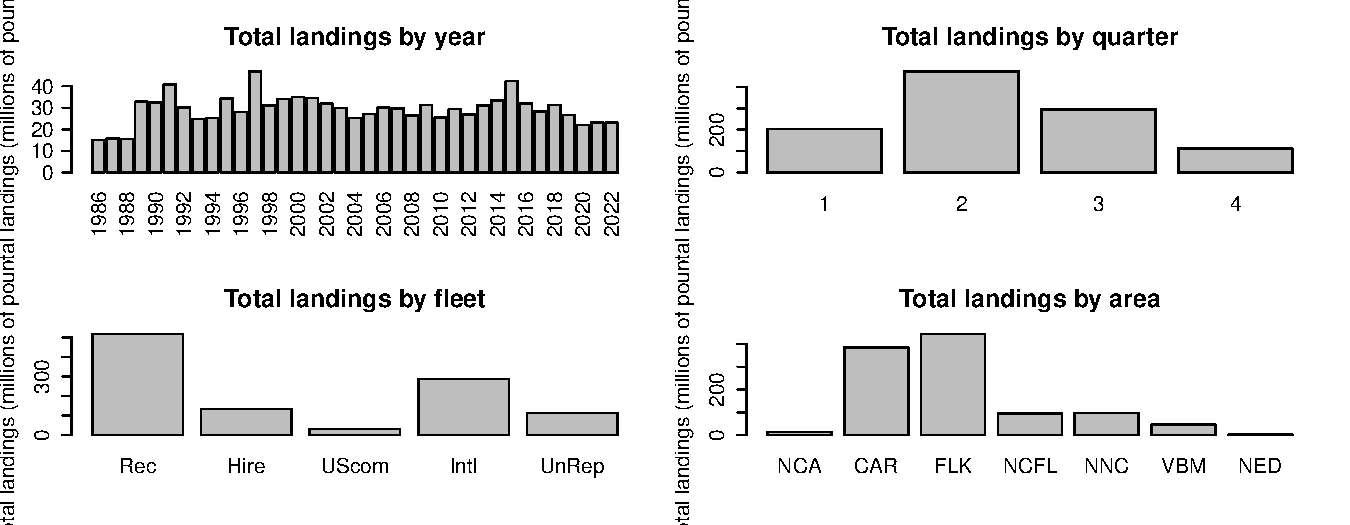
\includegraphics{compile_all_data_files/figure-pdf/unnamed-chunk-8-1.pdf}

The total catch in the regions analyzed is highly variable but
relatively stable over time with a slight decrease in recent years. Most
of the catch is caught in quarter 2 (March - May). The largest sector is
the U.S. private recreational sector, followed by international fleets
(all types), the for-hire fleet and then the U.S. commercial fleet. Most
of the fishing activity takes place in the Florida Keys and the Greater
Caribbean, with other regions contributing much less.

\begin{Shaded}
\begin{Highlighting}[]
\FunctionTok{par}\NormalTok{(}\AttributeTok{mfrow =} \FunctionTok{c}\NormalTok{(}\DecValTok{1}\NormalTok{, }\DecValTok{1}\NormalTok{), }\AttributeTok{mar =} \FunctionTok{c}\NormalTok{(}\DecValTok{2}\NormalTok{, }\DecValTok{5}\NormalTok{, }\DecValTok{3}\NormalTok{, }\DecValTok{1}\NormalTok{))}
\NormalTok{tab }\OtherTok{\textless{}{-}} \FunctionTok{tapply}\NormalTok{(d}\SpecialCharTok{$}\NormalTok{Catch\_lbs, }\FunctionTok{list}\NormalTok{(d}\SpecialCharTok{$}\NormalTok{Fleet, d}\SpecialCharTok{$}\NormalTok{Area), sum, }\AttributeTok{na.rm =}\NormalTok{ T)}\SpecialCharTok{/}\DecValTok{10}\SpecialCharTok{\^{}}\DecValTok{6}
\FunctionTok{barplot}\NormalTok{(tab, }\AttributeTok{beside =}\NormalTok{ T, }\AttributeTok{col =} \FunctionTok{c}\NormalTok{(}\StringTok{"navy"}\NormalTok{, }\StringTok{"blue"}\NormalTok{, }\StringTok{"darkturquoise"}\NormalTok{, }\StringTok{"red"}\NormalTok{, }\StringTok{"pink"}\NormalTok{)}
\NormalTok{        , }\AttributeTok{legend =} \FunctionTok{rownames}\NormalTok{(tab),}
        \AttributeTok{main =} \StringTok{"Total dolphin catch by area and fleet"}\NormalTok{, }
        \AttributeTok{ylab =} \StringTok{"total catch (millions of pounds)"}\NormalTok{)}
\end{Highlighting}
\end{Shaded}

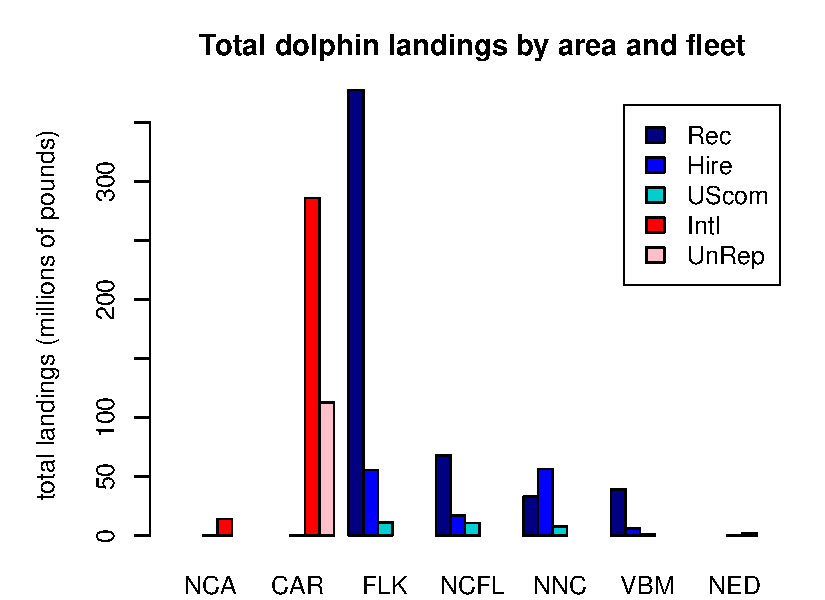
\includegraphics{compile_all_data_files/figure-pdf/unnamed-chunk-9-1.pdf}

As expected, U.S. recreational fishing (private and for-hire) only takes
place in the four U.S. EEZ regions (FLK, NCFL, NNC and VBM). The U.S.
commercial fishery operates largely in those four U.S. EEZ regions, with
small amounts of catch in the high seas of NCA, CAR and NED regions.
International catches occur largely in the Caribbean, with lesser
amounts in the NCA and NED high seas regions.

\begin{Shaded}
\begin{Highlighting}[]
\NormalTok{tab }\OtherTok{\textless{}{-}} \FunctionTok{tapply}\NormalTok{(d}\SpecialCharTok{$}\NormalTok{Catch\_lbs, }\FunctionTok{list}\NormalTok{(d}\SpecialCharTok{$}\NormalTok{Quarter, d}\SpecialCharTok{$}\NormalTok{Area), sum, }\AttributeTok{na.rm =}\NormalTok{ T)}\SpecialCharTok{/}\DecValTok{10}\SpecialCharTok{\^{}}\DecValTok{6}
\NormalTok{tabp }\OtherTok{\textless{}{-}} \FunctionTok{apply}\NormalTok{(tab, }\DecValTok{2}\NormalTok{, }\ControlFlowTok{function}\NormalTok{(x) x }\SpecialCharTok{/} \FunctionTok{sum}\NormalTok{(x, }\AttributeTok{na.rm =}\NormalTok{ T))}

\FunctionTok{par}\NormalTok{(}\AttributeTok{mar =} \FunctionTok{c}\NormalTok{(}\DecValTok{2}\NormalTok{, }\DecValTok{4}\NormalTok{, }\DecValTok{3}\NormalTok{, }\DecValTok{1}\NormalTok{))}
\FunctionTok{barplot}\NormalTok{(tabp, }\AttributeTok{beside =}\NormalTok{ T, }\AttributeTok{col =} \FunctionTok{rainbow}\NormalTok{(}\DecValTok{4}\NormalTok{, }\AttributeTok{end =} \FloatTok{0.8}\NormalTok{), }
        \AttributeTok{legend =} \FunctionTok{c}\NormalTok{(}\StringTok{"winter (DJF)"}\NormalTok{, }\StringTok{"spring (MAM)"}\NormalTok{, }\StringTok{"summer (JJA)"}\NormalTok{, }\StringTok{"fall (SON)"}\NormalTok{), }
        \AttributeTok{args.legend =} \FunctionTok{list}\NormalTok{(}\AttributeTok{x =} \DecValTok{15}\NormalTok{, }\AttributeTok{y =} \FloatTok{0.7}\NormalTok{, }\AttributeTok{bty =} \StringTok{"n"}\NormalTok{), }
        \AttributeTok{main =} \StringTok{"Total dolphin catch by area and season"}\NormalTok{, }
        \AttributeTok{ylab =} \StringTok{"proportion of catch"}\NormalTok{)}
\end{Highlighting}
\end{Shaded}

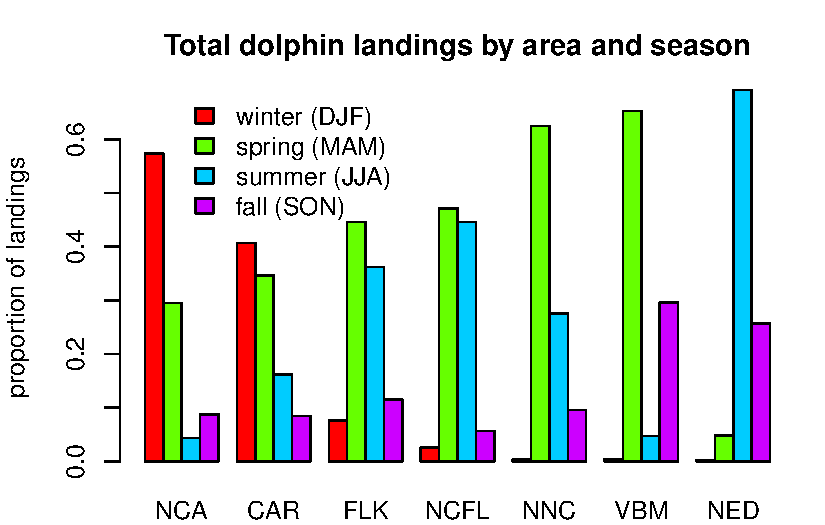
\includegraphics{compile_all_data_files/figure-pdf/unnamed-chunk-10-1.pdf}

This plot shows the seasonal movements of dolphin across the different
regions, as expressed through the proportion of catch that occurs in
each quarter within each area. In the NCA and CAR regions, most of the
catch occurs in winter, whereas in the U.S. South Atlantic regions, most
of the catch occurs in spring and summer. In the U.S. Mid-Atlantic the
catch also occurs largely in spring, and also fall. In the NED region
most of the catch occurs in summer.

\begin{Shaded}
\begin{Highlighting}[]
\NormalTok{tab }\OtherTok{\textless{}{-}} \FunctionTok{tapply}\NormalTok{(d}\SpecialCharTok{$}\NormalTok{Catch\_lbs, }\FunctionTok{list}\NormalTok{(d}\SpecialCharTok{$}\NormalTok{Year, d}\SpecialCharTok{$}\NormalTok{Fleet), sum, }\AttributeTok{na.rm =}\NormalTok{ T)}\SpecialCharTok{/}\DecValTok{10}\SpecialCharTok{\^{}}\DecValTok{6}

\FunctionTok{par}\NormalTok{(}\AttributeTok{mar =} \FunctionTok{c}\NormalTok{(}\DecValTok{2}\NormalTok{, }\DecValTok{4}\NormalTok{, }\DecValTok{3}\NormalTok{, }\DecValTok{1}\NormalTok{))}
\FunctionTok{matplot}\NormalTok{(}\FunctionTok{rownames}\NormalTok{(tab), tab, }
        \AttributeTok{col =} \FunctionTok{c}\NormalTok{(}\StringTok{"navy"}\NormalTok{, }\StringTok{"blue"}\NormalTok{, }\StringTok{"darkturquoise"}\NormalTok{, }\StringTok{"red"}\NormalTok{, }\StringTok{"pink"}\NormalTok{), }
        \AttributeTok{type =} \StringTok{"l"}\NormalTok{, }\AttributeTok{lwd =} \DecValTok{2}\NormalTok{, }\AttributeTok{lty =} \FunctionTok{c}\NormalTok{(}\FunctionTok{rep}\NormalTok{(}\DecValTok{1}\NormalTok{, }\DecValTok{3}\NormalTok{), }\DecValTok{2}\NormalTok{, }\DecValTok{2}\NormalTok{), }
        \AttributeTok{main =} \StringTok{"Total annual dolphin catch by fleet"}\NormalTok{, }\AttributeTok{xlab =} \StringTok{""}\NormalTok{,}
        \AttributeTok{ylab =} \StringTok{"total catch (millions of pounds)"}\NormalTok{)}
\FunctionTok{legend}\NormalTok{(}\DecValTok{2002}\NormalTok{, }\DecValTok{25}\NormalTok{, }\AttributeTok{lwd =} \DecValTok{2}\NormalTok{, }\AttributeTok{lty =} \FunctionTok{c}\NormalTok{(}\FunctionTok{rep}\NormalTok{(}\DecValTok{1}\NormalTok{, }\DecValTok{3}\NormalTok{), }\DecValTok{2}\NormalTok{, }\DecValTok{2}\NormalTok{), }\AttributeTok{bty =} \StringTok{"n"}\NormalTok{, }
       \FunctionTok{c}\NormalTok{(}\StringTok{"U.S. private rec"}\NormalTok{, }\StringTok{"U.S. for{-}hire"}\NormalTok{, }\StringTok{"U.S. commercial"}\NormalTok{, }
         \StringTok{"International"}\NormalTok{, }\StringTok{"Unreported"}\NormalTok{),}
       \AttributeTok{col =} \FunctionTok{c}\NormalTok{(}\StringTok{"navy"}\NormalTok{, }\StringTok{"blue"}\NormalTok{, }\StringTok{"darkturquoise"}\NormalTok{, }\StringTok{"red"}\NormalTok{, }\StringTok{"pink"}\NormalTok{))}
\end{Highlighting}
\end{Shaded}

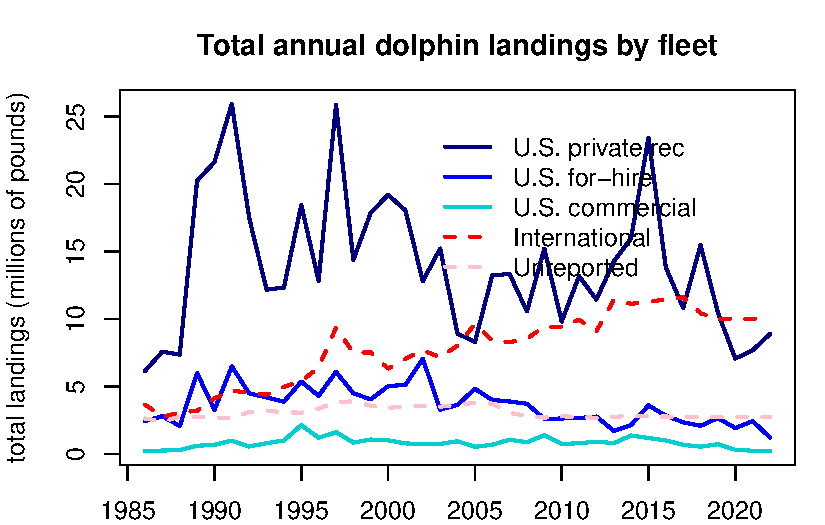
\includegraphics{compile_all_data_files/figure-pdf/unnamed-chunk-11-1.pdf}

This plot shows the time series of total annual dolphin catches by
fleet. We can compare these figures with the plots from the previous
chapters to ensure the data were processed correctly. The magnitude and
variability of the landings match the expectations.

\begin{Shaded}
\begin{Highlighting}[]
\CommentTok{\# output the final concatenated data file}
\FunctionTok{write.csv}\NormalTok{(d, }\AttributeTok{file =} \StringTok{"data/FINAL\_files/complete\_catch\_dataset\_09052025b.csv"}\NormalTok{, }\AttributeTok{row.names =} \ConstantTok{FALSE}\NormalTok{)}
\end{Highlighting}
\end{Shaded}



\backmatter


\end{document}
